%%%%%%%%%%%%%%%%%%%%%%%%%%%%%%%%%%%%%%%%%%%%%%%%%%%%%%%%%%%%%%%%%%%%%%
% Lớp 12 | Nguyên hàm, tích phân | Nguyên hàm
% Dạng 2D4?1-6: Toán thực tế áp dụng nguyên hàm
% Số câu: 99  (sinh tự động bởi tach_cau.py; từ nay thầy sửa trực tiếp file này)
%%%%%%%%%%%%%%%%%%%%%%%%%%%%%%%%%%%%%%%%%%%%%%%%%%%%%%%%%%%%%%%%%%%%%%

%%%%%%%%%%%%%%%% TRẮC NGHIỆM 4 PHƯƠNG ÁN %%%%%%%%%%%%%%%%

% nguồn: Phan1_Lop_12_Dai_so_Chuong_4
\begin{ex}%[2D4H1-6]%[ma:b11309f4]
	Giả sử một chất điểm chuyển động với gia tốc  tại thời điểm $t$ (giây) được xác định bởi công thức $a(t)=2t-1$ (m/s$^2$). Biết rằng vận tốc của chất điểm tại thời điểm ban đầu là $v_0=2$ (m/s$^2$). Vận tốc của chất điểm đó tại thời điểm $t$ (giây) là
	 \choice
		{$v(t)=2t^2-t+2$ (m/s$^2$)} 
		{\True $v(t)=t^2-t+2$ (m/s$^2$)} 
		 {$v(t)=2t^2-t$ (m/s$^2$)}
		{$v(t)=t^2-t$ (m/s$^2$)} 
	\loigiai{ 
		Ta có $v(t)=\displaystyle\int  (2t-1) \mathrm{\,d}t=t^2-t+C$.\\
		Ứng  với $v_0=2$ thi $t=0$ khi đó ta có $C=2$. Vậy $v(t)=t^2-t+2$ (m/s$^2$).
	} 
\end{ex}

% nguồn: Phan1_Lop_12_Dai_so_Chuong_4
\begin{ex}%[2D4V1-6]%[ma:cfb3ebd2]
	Sự sản sinh vi-rút Zika ngày thứ $t$ có số lượng là  $N(t)$ con, biết $N'(t)=\dfrac{1\,000}{t}$ và lúc đầu số lượng vi-rút Zika là $250\,000$ con. Tính số lượng vi-rút sau $10$ ngày.
	 \choice
		 {$272\,304$ con}
		{$212\,302$ con} 
		 {$242\,102$ con}
		{\True  $252\,302$ con}
	\loigiai{ 
		Ta  có
		\[N'(t)=\dfrac{1\,000}{t}\Rightarrow  N(t)=\displaystyle\int{\dfrac{1\,000}{t}\text{ d}t=1\,000\ln|t|}+C\Rightarrow N(t)=1\,000\ln |t|+C.\]
		Chọn $t=1\Rightarrow  N(1)=250\,000\Rightarrow C=250\,000$ $\Rightarrow N(t)=1\,000\ln |t|+250\,000$.\\
		Vậy số lượng vi-rút sau $10$ ngày là $N(10)=1\,000\ln 10+250\,000\approx 252\,302$. 
	} 
\end{ex}

% nguồn: Phan1_Lop_12_Dai_so_Chuong_4
\begin{ex}%[2D4V1-6]%[ma:4898e5c0]
	Một ô tô đang chạy với vận tốc $20~\mathrm{m/s} $ thì người người đạp phanh. Sau khi đạp phanh, ô tô chuyển động chậm dần đều với vận tốc $v(t)=-40t+20~\mathrm{m/s}$, trong đó $t$ là khoảng thời gian tính bằng giây kể từ lúc bằng đầu đạp phanh. Gọi $s(t)$ là quãng đường xe ô tô đi được trong  thời gian $t$ giây kể từ lúc đạp phanh. Hỏi từ lúc đạp phanh đến khi dừng hẳn, ô tô còn di chuyển bao nhiêu mét?
	\choice 
		{$5~\mathrm{cm}$} 
		{$7{,}5~\mathrm{m}$} 
		 {$\dfrac{5}{2}~\mathrm{m}$}
		 {\True $5~\mathrm{m}$}
	 \loigiai{
		Ta có 
		 $v(t)=-40t+20\Rightarrow s(t)=\displaystyle\int{v\left(t \right)}\mathrm{\,d}t=\displaystyle\int{\left(-40t+20\right)}\mathrm{\,d}t=-20t^2+20t+C$.\\
		$\Rightarrow s(t)=-20t^2+20t+C$.\\ 
		Chọn $t=0\Rightarrow s(0)=0$ $\Rightarrow C=0$ $\Rightarrow s(t)=-20t^2+20t$.\\ 
		Khi xe dừng hẳn thì  $v(t)=0\Leftrightarrow-40t+20=0\Rightarrow t=0{,}5$.\\
		Từ lúc đạp phanh đến khi dừng hẳn, ô tô còn di chuyển  được \[s\left(0{,}5\right)=-20\cdot\left(0{,}5\right)^2+20\cdot\left(0{,}5\right)=5~\mathrm{m}.\]
	 }
\end{ex}

% nguồn: Phan1_Lop_12_Dai_so_Chuong_4
\begin{ex}%[2D4V1-6]%[ma:87d05ca7]
	Người ta bơm nước vào một bồn chứa. Lúc đầu bồn không có nước. Mực nước trong bồn sau khi bơm phụ thuộc vào thời gian $t$ theo hàm số $h=h(t)$, trong đó $h$ tính bằng $\mathrm{cm}$, $t$ tính bằng giây. Biết rằng $h'(t)=\sqrt[3]{3t  + 8}$. Hỏi sau $10$ giây, mực nước trong bồn là bao nhiêu (làm tròn đến hàng phần trăm) ?
	\choice 
		{$25{,}6~\mathrm{cm}$} 
		 {$42{,}1~\mathrm{cm}$}
		 {$45{,}0~\mathrm{cm}$}
		{\True $27{,}94~\mathrm{cm}$} 
	\loigiai{ 
		Ta có $h(t) =\displaystyle \int h'(t)\,\mathrm{\,d}t =  \displaystyle \int \sqrt[3]{3t + 8}\,\mathrm{\,d}t.$\\
		Đặt $u=3t+8\Rightarrow\mathrm{\,d}u=3\,\mathrm{\,d}t \Rightarrow \mathrm{\,d}t=\dfrac{1}{3}\mathrm{\,d}u  $, ta được
		\[h(t)=\displaystyle\int \sqrt[3]{u} \cdot \dfrac{1}{3}\,du =  \dfrac{1}{3} \cdot \dfrac{3}{4}u^{4/3}+C=\dfrac{1}{4}(3t+8)\cdot \sqrt[3]{3t+8}+C.\]
		Vì $h(0)=\dfrac{1}{4}\cdot8\cdot\sqrt[3]{8}+C=4+C$ và $h(0)=0$  nên $C=-4$.\\
		Vậy $h(t)=\dfrac{1}{4}(3t+8)\cdot\sqrt[3]{3t+8}-4$.\\ 
		Từ  đó tính được $h(10)\approx 27{,}94~\mathrm{cm}$.
	} 
\end{ex}

% nguồn: Phan1_Lop_12_Dai_so_Chuong_4
\begin{ex}%[2D4V1-6]%[ma:c7186750]
	Bạn Minh Hiền ngồi trên máy bay đi du lịch thế giới với vận tốc chuyển động của máy  bay theo phương trình là $v\left(t\right)=3{t^2}+5~\mathrm{m/s}$. Quãng đường máy bay bay từ giây thứ $4$ đến giây thứ $10$ là
	 \choice
		 {$36~\mathrm{m}$}
		 {$252~\mathrm{m}$}
		{$1\,134~\mathrm{m}$} 
		{\True  $966~\mathrm{m}$}
	 \loigiai{
		Ta  có
		\[v(t)=3{t^2}+5\Rightarrow s(t)=\displaystyle\int{v(t)\text{  d}t}=\displaystyle\int{\left(3t^2+5\right)}\text{ d}t=t^3+5t+C\Rightarrow s(t)={t^3}+5t+C.\]
		Chọn $t=0\Rightarrow s(0)=0\Rightarrow C=0\Rightarrow s(t)={t^3}+5t$.\\ 
		Quãng đường máy bay bay  từ giây thứ $4$ là $s(4)=4^3+5\cdot 4=84~\mathrm{m}$.\\
		Quãng đường máy bay bay  từ giây thứ $10$ là $s(10)=10^3+5\cdot 10=1\,050~\mathrm{m}$.\\
		Quãng  đường máy bay bay từ giây thứ $4$ đến giây thứ $10$ là
		 $s(10)-s(4)=966~\mathrm{m}$.
	 }
\end{ex}

% nguồn: Phan1_Lop_12_Dai_so_Chuong_4
\begin{ex}%[2D4V1-6]%[ma:a7073749]
	Một bác thợ xây bơm nước vào bể chứa nước. Gọi $h(t)$ là thể tích  nước (tính bằng $\mathrm{m^3}$) bơm được sau $t$ giây. Biết $h'(t) = 3a t^2 + bt$ và ban đầu bể không có nước. Sau $5$ giây thì thể tích là $150~\mathrm{m^3}$, sau $10$ giây là $1100~\mathrm{m^3}$. Tính thể tích nước trong bể sau $20$ giây.
	\choice 
		{\True $8\,400~\mathrm{m^3}$} 
		 {$4\,200~\mathrm{m^3}$}
		 {$7\,260~\mathrm{m^3}$}
		{$8\,560~\mathrm{m^3}$} 
	 \loigiai{
		Ta có $h(t)=\int (3a t^2  + bt)\,\mathrm{\,d}t=a t^3+\dfrac{1}{2}bt^2+C$.\\
		Vì $h(0)=0\Rightarrow C=0$ nên $h(t)=at^3+\dfrac{1}{2}bt^2$.\\ 
		 Ta có hệ \[\heva{&125a+\dfrac{25}{2}b=150\\
		&1\,000a+50b=1\,100}\Rightarrow\heva{&a=1\\&b=2}\Rightarrow h(t)=t^3+t^2.\] 
		 Vậy $h(20)=20^3+20^2=8\,000+400=8\,400~\mathrm{m^3}$.
	} 
\end{ex}

% nguồn: Phan1_Lop_12_Dai_so_Chuong_4
\begin{ex}%[2D4V1-6]%[ma:ca64f4ea]
	Trong một đợt xả lũ, nhà máy thủy điện đã xả lũ trong $40$ phút với tốc độ lưu lượng nước là $h'(t)=10t+500 ~\mathrm{m^3/s} $. Hỏi sau thời gian xả lũ trên thì hồ thoát nước của nhà  máy đã thoát đi một lượng nước là bao nhiêu?
	\begin{center}
		\begin{tikzpicture}[scale=0.7,>=stealth,line join=round,line cap=round,font=\footnotesize]
				 \path (0,0) coordinate (dt);
				\fill  [cyan!90!black!60] (dt)++(2.14,3.2)--++(11.41,0)--++(.57,-1.2)--++(4.66,0)--++(0,-2)--++(-18.78,0)--cycle;
				\draw  [double,double distance=2pt,double=yellow] (dt)++(12.3,3.65) circle (.35);
				 \draw [fill=brown!30] (dt)--++(0,2)--++(.74,2.31)--++(1.4,0)--++(1.75,-3.15)
					.. controls +(9,-.15) and +(-.8,1.4)..  ++(13.52,-.82)--++(1.38,0)--++(0,-.34)--cycle;
				 \draw [fill=gray] (dt)++(10.66,.66)--++(0,.95)--++(1.08,0)--++(.53,-.4)--++(2.22,0)--++(.26,-.56)--++(-.9,0)--++(-.26,.21)--++(-1.72,0)--++(-.26,-.21)--cycle
					(dt)++(10.66,1.98)--++(0,1.67)--++(2.65,0)--++(1,-2.09)--++(-1.61,0)--++(-.53,.4)--cycle; 
				\draw [double,double distance=3pt] (dt)++(12.3,3.65)  circle (.8);
				\draw [fill=white] (dt)++(12.3,3.65)++(.37,0)  rectangle ++(-.74,-1.35);
				\draw  [<-,double,double distance=2pt,double=yellow] (dt)++(12.3,3.65)--++(0,-2.17) circle (2pt);
				\draw  (dt)
					 +(6.4,3.1) node [white,scale=3.5] {$\downarrow$}
					 +(10.08,1.77) node [white,scale=3.5,rotate=90] {$\downarrow$}
					 +(10.45,4.2) node [scale=3.5,rotate=-90] {$\downarrow$}
					+(8.2,4.2) node [align=center] {\bf Máy \\  \bf phát điện}
					+(6.4,1.69) node [align=center] {\bf  Hồ chứa};
				\draw [<-,line width=2pt] (dt)++(12.3,3.65)++(0,-2.17)++(-.1,-.1)--++(-2,-.75) node [left] {\bf  Turbine};
				\draw (dt) ++(30:2) node {\bf  Đập};
			\end{tikzpicture}
	\end{center}
	 \choice
		 {$5\cdot10^4~\mathrm{(m^3)}$}
		{$4\cdot10^6~\mathrm{(m^3)}$} 
		 {\True $3\cdot10^3~\mathrm{(m^3)}$}
		 {$6\cdot10^6~\mathrm{(m^3)}$}
	 \loigiai{
		 Ta có
		\[h'(t)=10t+500\Rightarrow h(t)=\displaystyle\int{(10t+500)}\text{  d}x=5{t^2}+500t+C\Rightarrow h(t)=5t^2+500t+C.\]
		Chọn $t=0\Rightarrow h(0)=0\Rightarrow C=0\Rightarrow h(t)=5{t^2}+500t$.\\ 
		Thủy điện đã xả lũ trong $40$ phút=$2\,400$  giây thì thoát đi một lượng nước là
		 \[h(2\,400)={{5\cdot 2\,400}^2}+500\cdot 2\,400={{3\cdot 10}^3}~\mathrm{(m^3)}.\]
	} 
\end{ex}

% nguồn: Phan1_Lop_12_Dai_so_Chuong_4
\begin{ex}%[2D4V1-6]%[ma:835b94f4]
	Một vật chuyển động với vận tốc $v(t)~\mathrm{m/s}$ có gia tốc $v'(t)=\dfrac{3}{t+1}~\mathrm{m/s^2}$. Vận tốc ban đầu của vật là $6~\mathrm{m/s} $. Hỏi vận tốc của vật sau $10$ giây (làm tròn đến kết quả đến  hàng phần mười) có giá trị bằng bao nhiêu?
	 \choice
		 {$5~\mathrm{m}$}
		 {\True $13{,}2~\mathrm{m}$}
		{$8~\mathrm{m}$} 
		{$7~\mathrm{m}$} 
	\loigiai{ 
		 Giả sử tại thời điểm ban đầu $t=0; ~v(0)=6~\mathrm{m/s}$.\\
		Ta có $v(0)=6\,(m/s)\Rightarrow v(t)=\displaystyle\int{v'(t)}\mathrm{\,d}t=\displaystyle\int{\dfrac{3}{t+1}\mathrm{\,d}t=3\ln  |t+1|+C}$.\\
		 $v(0)=6\Rightarrow C=6\Rightarrow v(t)=3\ln |t+1|+6\Rightarrow v(10)=3\ln 11+6\approx 13{,}2~\mathrm{m/s}$
	} 
\end{ex}

% nguồn: Phan1_Lop_12_Dai_so_Chuong_4
\begin{ex}%[2D4V1-6]%[ma:3fafc1aa]
	Gọi $h(t)$ $~\mathrm{m}$ là mực nước  ở bồn chứa sau khi bơm nước được t giây. Biết rằng \break$h'(t)=\dfrac{1}{5}\sqrt[3]t\text{ }~\mathrm{m/s}$
	và lúc đầu bồn không có nước. Tìm mức nước ở  bồn sau khi bơm nước được $6$ giây (làm tròn kết quả đến hàng phần trăm).
	 \choice
		{$2{,}64~\mathrm{m}$} 
		{$1{,}22~\mathrm{m}$} 
		{$2{,}22~\mathrm{m}$} 
		{\True  $1{,}64~\mathrm{m}$}
	 \loigiai{
		Ta có 
		\begin{align*}
			 h'(t)&=\dfrac{1}{5}\sqrt[3]t\\
			\Rightarrow  h(t)&=\displaystyle\int{\dfrac{1}{5}\sqrt[3]t}\mathrm{\,d}t=\dfrac{1}{5}\displaystyle\int{{t^{\tfrac{1}{3}}}}\mathrm{\,d}t\\
			 &=\dfrac{1}{5}\dfrac{{t^{\tfrac{1}{3}+1}}}{\dfrac{1}{3}+1}+C\\
			&=\dfrac{3}{20}t\sqrt[3]t+C. 
		\end{align*}
		Chọn $t=0\Rightarrow h(0)=0\Rightarrow  C=0$ $\Rightarrow h(t)=\dfrac{3}{20}t\sqrt[3]t$.\\
		Vậy mức nước ở bồn sau khi bơm nước được $6$ giây  là $h(6)=\dfrac{3}{20}\cdot6\sqrt[3]6\approx 1{,}64~\mathrm{m}$.
	 }
\end{ex}

% nguồn: Phan1_Lop_12_Dai_so_Chuong_4
\begin{ex}%[2D4V1-6]%[ma:1c4d8235]
	Một quả bóng được ném lên từ độ cao $20~\mathrm{m}$ với vận tốc được tính bởi công thức\break$v(t)=-10t+16~\mathrm{m/s}$. Công  thức nào sau đây tính độ cao của quả bóng theo thời gian $t$?
	\choice 
		{$h(t)=-5t^2+16t+C$} 
		{\True $h(t)=-5t^2+16t+20$} 
		{$h(t)=5t^2-16t+20$} 
		{$h(t)=5t^2-16t+C$} 
	\loigiai{ 
		 Ta có
		\[v(t)=\dfrac{\mathrm{\,d}h}{\mathrm{\,d}t}=-10t+16\Rightarrow  h(t) =\displaystyle\int v(t)\,\mathrm{\,d}t=\displaystyle\int (-10t+16)\,\mathrm{\,d}t=-5t^2+16t+C.\]
		Vì ban đầu quả bóng ở  độ cao $20\,\mathrm{m}$, tức là $h(0)=20$ nên
		$h(0)=-5\cdot 0^2+16\cdot 0+C=C=20$.\\ 
		 Vậy công thức cần tìm là $h(t)=-5t^2+16t+20.$
	} 
\end{ex}

% nguồn: Phan1_Lop_12_Dai_so_Chuong_4
\begin{ex}%[2D4V1-6]%[ma:7c4330d7]
	Một ô tô đang chạy với  vận tốc $70~\mathrm{km/h}$ thì hãm phanh và chuyển động chậm dần đều với tốc độ $v\left(t \right)=-10t+30~\mathrm{m/s}$. Tính quãng đường ô tô đi được sau $3$ giây kể từ khi hãm phanh.
	\choice 
		 {$51~\mathrm{m}$}
		{$43~\mathrm{m}$} 
		{$54~\mathrm{m}$} 
		{\True $45~\mathrm{m}$} 
	\loigiai{ 
		Gọi $s(t)$ là quãng đường xe ô tô đi được trong $t$ giây kể từ khi hãm phanh.\\ 
		Ta  có
		\[s(t)=\displaystyle\int(-10t+30)\mathrm{\,d}t=-5t^2+30t+C.\] 
		Do $s(0)=0\Rightarrow C=0$.\\ 
		Khi đó \[s(t)=-5{t^2}+30t\Rightarrow s(3)=-5\cdot  9+30\cdot 3=45~\mathrm{m}.\]
	 }
\end{ex}

% nguồn: Phan1_Lop_12_Dai_so_Chuong_4
\begin{ex}%[2D4V1-6]%[ma:8a5398fb]
	Mực nước trong hồ chứa của nhà máy điện thủy triều thay đổi theo thời gian $t$ trong ngày do thủy triều lên xuống. Tốc độ thay đổi của mực nước được cho bởi $h'(t)=\dfrac{1}{90}(t^2-17t+60)$, $0\le t\le 24$, trong đó $h'(t)$ tính bằng $\mathrm{m/h}$, $t$ tính bằng giờ. Biết  rằng $h(0) = 8~\mathrm{m}$. Hỏi mực nước trong hồ cao nhất và thấp nhất là bao nhiêu?
	\begin{center}
		\begin{tikzpicture}[scale=0.7,>=stealth,line join=round,line cap=round,font=\footnotesize]
				\path (0,0) coordinate  (dtd);
				\fill [cyan!90!black!60] (dtd)++(2.14,3.2)--++(11.41,0)--++(.57,-1.2)--++(4.66,0)--++(0,-2)--++(-18.78,0)--cycle; 
				\draw [double,double  distance=2pt,double=yellow] (dtd)++(12.3,3.65) circle (.35);
				 \draw [fill=brown!30] (dtd)--++(0,2)--++(.74,2.31)--++(1.4,0)--++(1.75,-3.15)
					.. controls +(9,-.15)  and +(-.8,1.4).. ++(13.52,-.82)--++(1.38,0)--++(0,-.34)--cycle;
				\draw [fill=gray] (dtd)++(10.66,.66)--++(0,.95)--++(1.08,0)--++(.53,-.4)--++(2.22,0)--++(.26,-.56)--++(-.9,0)--++(-.26,.21)--++(-1.72,0)--++(-.26,-.21)--cycle 
					(dtd)++(10.66,1.98)--++(0,1.67)--++(2.65,0)--++(1,-2.09)--++(-1.61,0)--++(-.53,.4)--cycle; 
				\draw [double,double distance=3pt] (dtd)++(12.3,3.65)  circle (.8);
				\draw [fill=white] (dtd)++(12.3,3.65)++(.37,0) rectangle  ++(-.74,-1.35);
				 \draw [<-,double,double distance=2pt,double=yellow] (dtd)++(12.3,3.65)--++(0,-2.17) circle (2pt);
				\draw (dtd) 
					+(6.4,3.1) node [white,scale=3.5]  {$\downarrow$}
					+(16.96,2.67) node [white,scale=3.5] {$\downarrow$} 
					+(10.08,1.77) node  [white,scale=3.5,rotate=90] {$\downarrow$}
					+(10.45,4.2)  node [scale=3.5,rotate=-90] {$\downarrow$}
					+(16.96,4.15) node [red,align=center] {\bf Thủy  triều \\ \bf xuống}
					+(8.2,4.2) node [align=center] {\bf Máy \\ \bf  phát điện}
					 +(6.4,1.69) node [align=center] {\bf Hồ chứa};
				\draw [<-,line width=2pt] (dtd)++(12.3,3.65)++(0,-2.17)++(-.1,-.1)--++(-2,-.75)  node [left] {\bf Turbine};
				\draw  (dtd) ++(30:2) node {\bf Đập};
				\begin{scope}[shift={(0,-6)}]
					\path (0,0)  coordinate (dtd);
					\fill [cyan!90!black!60]  (dtd)++(2.14,2.2)--++(11.41,0)
						--++(-0.57,1)--++(5.8,0)--++(0,-3)--++(-18.78,0)--cycle; 
					\draw [double,double distance=2pt,double=yellow] (dtd)++(12.3,3.65)  circle (.35);
					\draw  [fill=brown!30] (dtd)--++(0,2)--++(.74,2.31)--++(1.4,0)--++(1.75,-3.15)
						.. controls  +(9,-.15) and +(-.8,1.4).. ++(13.52,-.82)--++(1.38,0)--++(0,-.34)--cycle;
					\draw [fill=gray] (dtd)++(10.66,.66)--++(0,.95)--++(1.08,0)--++(.53,-.4)--++(2.22,0)--++(.26,-.56)--++(-.9,0)--++(-.26,.21)--++(-1.72,0)--++(-.26,-.21)--cycle 
						 (dtd)++(10.66,1.98)--++(0,1.67)--++(2.65,0)--++(1,-2.09)--++(-1.61,0)--++(-.53,.4)--cycle;
					\draw [double,double distance=3pt] (dtd)++(12.3,3.65)  circle (.8);
					\draw [fill=white] (dtd)++(12.3,3.65)++(.37,0) rectangle  ++(-.74,-1.35);
					\draw [->,double,double  distance=2pt,double=yellow] (dtd)++(12.3,3.65)--++(0,-2.17) circle (2pt);
					\draw  (dtd)
						+(6.4,3.1) node  [white,scale=3.5] {$\downarrow$}
						+(16.96,2.67) node  [white,scale=3.5] {$\uparrow$}
						+(10.08,1.77) node [white,scale=3.5,rotate=90] {$\uparrow$} 
						+(10.45,4.2)  node [scale=3.5,rotate=-90] {$\downarrow$}
						+(16.96,4.15) node [red,align=center] {\bf Thủy triều \\ \bf lên} 
						+(8.2,4.2) node [align=center] {\bf Máy  \\ \bf phát điện}
						+(6.4,1.69) node [align=center] {\bf  Hồ chứa};
					\draw [<-,line width=2pt] (dtd)++(12.3,3.65)++(0,-2.17)++(-.1,-.1)--++(-2,-.75)  node [left] {\bf Turbine};
					\draw (dtd) ++(30:2) node {\bf Đập}; 
				\end{scope}
			\end{tikzpicture}
	\end{center}
	 \choice
		{\True  $20{,}88~\mathrm{m}$; $8~\mathrm{m}$}
		{$10{,}88~\mathrm{m}$;  $4~\mathrm{m}$}
		 {$12{,}88~\mathrm{m}$; $7~\mathrm{m}$}
		 {$20~\mathrm{m}$; $6~\mathrm{m}$}
	\loigiai{ 
		 Ta có
		\begin{align*}
			h^{\prime}(t)&=\dfrac{1}{90}\left(t^2-17  t+60\right)\\
			 \Rightarrow h(t)&=\dfrac{1}{90} \displaystyle\int\left(t^2-17 t+60\right) \mathrm{d} t=\dfrac{1}{90}\left(\dfrac{1}{3} t^3-\dfrac{17}{2} t^2+60 t\right)+C.
		\end{align*}
		Khi đó $h(t)=\dfrac{1}{90}\left(\dfrac{1}{3} t^3-\dfrac{17}{2} t^2+60  t\right)+C$.\\
		Tại thời điểm $t=0$, mực nước trong hồ chứa cao $ 8 \mathrm{~m} $ nên  $h(0)=8 \Rightarrow C=8$.\\
		$\Rightarrow h(t)=\dfrac{1}{90}\left(\dfrac{1}{3} t^3-\dfrac{17}{2} t^2+60 t\right)+8$ $(0 \leq  t \leq 24)$.\\
		Ta có $h^{\prime}(t)=0 \Leftrightarrow t^2-17 t+60=0 \Leftrightarrow\left[\begin{array}{l}t=5 \\ t=12.
	\end{array}\right.$\\
	 Lập bảng biến thiên
	\begin{center}
		
\begin{tikzpicture}
				\tkzTabInit[nocadre=true,lgt=1.2,espcl=2.5,deltacl=0.5] 
					 {$t$/.7,$h'(t)$/.7,$h (t)$/2}
					 {0,5,12,24}
				\tkzTabLine{,+,z,-,z,+,} 
				\tkzTabVar 
					{-/$8$,+/  $\dfrac{1019}{108}$,-/ $\dfrac{44}{5}$,+/ $\dfrac{104}{5}$}
			\end{tikzpicture}
	\end{center}
	Vậy, mực nước trong hồ cao nhất  là $\dfrac{104}{5}=20{,}88~\mathrm{m} $ và thấp nhất là $ 8~\mathrm{m} $.
 }
\end{ex}

% nguồn: Phan1_Lop_12_Dai_so_Chuong_4
\begin{ex}%[2D4C1-6]%[ma:ba8400f9]
	Một bác thợ xây bơm nước  vào bể chứa nước. Gọi $h(t)$ là thể tích nước bơm được sau $t$ giây. Cho biết $h'(t) = 3a t^2 + bt$ (đơn vị: $\mathrm{m^3/s}$) và ban đầu bể không có nước. Sau $5$ giây thì thể tích nước trong bể là $150~\mathrm{m^3}$. Sau $10$ giây là $1100~\mathrm{m^3}$. Hỏi sau $20$ giây thì thể tích nước trong bể là bao nhiêu?
	 \choice
		 {\True $8\,400~\mathrm{m^3}$}
		 {$6\,400~\mathrm{m^3}$}
		{$6\,000~\mathrm{m^3}$} 
		 {$4\,200~\mathrm{m^3}$}
	\loigiai{ 
		Ta  có
		\[h'(t)=3at^2+bt\Rightarrow h(t)=\int(3at^2+bt)\,\mathrm{\,d}t=at^3+\dfrac{1}{2}bt^2+C.\] 
		Vì ban đầu bể không có nước  ($h(0)=0$) nên $C=0$.\\
		Do  đó $h(t)=at^3+\dfrac{1}{2}bt^2.$\\
		Từ giả  thiết $h(5)=150\Rightarrow 125a+\dfrac{25}{2}b=150$\hfill(1)\\
		$h(10)=1\,100\Rightarrow 1\,000a+50b=1\,100$\hfill(2)\\ 
		Giải hệ phương trình (1) và (2): 
		\[\heva{&125a+\dfrac{25}{2}b=150\\ 
		 &1\,000a+50b=1\,100}\Rightarrow\heva{&a=1\\&b=2.}\]
		Thay vào biểu thức $h(t)$:  $h(t)=t^3+t^2$.\\
		Vậy thể tích nước của  bể sau $20$ giây là
		 \[h(20)=20^3+20^2=8\,000+400=8\,400~\mathrm{m}^3.\]
	} 
\end{ex}

% nguồn: Phan1_Lop_12_Dai_so_Chuong_4
\begin{ex}%[2D4B1-6]%[ma:6a27bb72]
	Một vật chuyển động có gia tốc là $a\left(t\right)=3 t^2+t$ (m/s$^2$). Biết rằng vận tốc ban đầu của vật là $2$ m/s. Vận tốc của  vật đó sau $2$ giây là
	\choice 
		{$8$ m/s} 
		{$10$ m/s} 
		{\True $12$  m/s}
		{$16$ m/s} 
	 \loigiai{
		Vận tốc của vật là $v(t)=\displaystyle  \int \left(3 t^2+t\right) \mathrm{\,d}t =t^3+\dfrac{1}{2}t^2+C$.\\
		Vì  vận tốc tốc ban đầu của vật là $2$ m/s nên $v(0)=2 \Leftrightarrow 0^3+\dfrac{1}{2}\cdot 0^2+C=2 \Leftrightarrow C=2$.\\
		Suy ra $v(t)=t^3+\dfrac{1}{2}t^2+2$.\\ 
		Vận tốc của vật đó sau $2$ giây  là $v(2)=2^3+\dfrac{1}{2}\cdot 2^2+2=12$ (m/s).
	} 
\end{ex}


%%%%%%%%%%%%%%%% ĐÚNG/SAI %%%%%%%%%%%%%%%%

% nguồn: Phan1_Lop_12_Dai_so_Chuong_4
\begin{ex}%[2D4H1-6]%[ma:fefa7f74]
	Trong dây chuyền sản xuất sữa chua hiện đại của một nhà máy thực phẩm, từng giọt sữa chua âm thầm chuyển mình dưới tác động của hàng triệu vi khuẩn Lactic, những \lq \lq nghệ nhân tí hon \rq \rq kiến tạo vị  chua thanh đặc trưng. Mật độ vi khuẩn (số triệu tế bào trên mỗi ml sữa chua) tại thời điểm $t$ (giờ) được kí hiệu là $N(t)$. Ban đầu ($t=0$ giờ), mật độ vi khuẩn đo được là $N(0)=10$ triệu tế bào/ml. Do sự thay đổi về nguồn dinh dưỡng (đường lactose giảm) và độ pH (axit lactic tăng) nên tốc độ thay đổi mật độ vi khuẩn $N'(t)$ (đơn vị: triệu tế bào/ml mỗi giờ) được mô hình hóa bởi công thức $N'(t) = 18t - 3t^2$ (triệu tế bào/ml mỗi giờ) với $t$ là thời gian tính bằng giờ $(0 \leq t \leq 7)$.
	\choiceTF 
		{\True $N'(1)=15$ triệu tế bào/ml  giờ}
		{$\displaystyle\int N'(t)  \mathrm{\,d}t=9t^2-t^3$}
		 {\True So với lúc ban đầu ($t=0$), mật độ vi khuẩn đã tăng thêm $108$ triệu tế bào/ml khi đến thời điểm $t=6$ giờ}
		{\True Tại thời điểm $t=7$ giờ, mật độ vi khuẩn trong $1$ ml sữa  chua là $108$ triệu tế bào/ml}
	\loigiai{ 
		\begin{itemchoice}
			\itemch Ta có $N'(1)=18\cdot 1-3\cdot  1^2=15$ triệu tế bào/ml giờ.
			\itemch Ta có $\displaystyle\int N'(t) \mathrm{\,d}t=\displaystyle\int \left(18t-3t^2\right) \mathrm{\,d}t=9t^2-t^3+C, \quad  (C \in \mathbb{R})$.
			\itemch 
			 Ta có $N(t)=9t^2-t^3+C$.\\
			 Vì $N(0)=10$ nên $C=10$.\\
			Do đó  $N(t)=9t^2-t^3+10$.\\
			Với $t=6$ ta có $N(6)=9\cdot 6^2-6^3+10=118$  triệu tế bào/ml giờ. \\
			Vậy từ  lúc ban đầu $(t=0)$ đến thời điểm $t=6$, mật độ vi khuẩn đã tăng thêm là $118-10=108$ triệu tế bào/ml giờ.
			\itemch Với $t=7$ ta  có $N(7)=9\cdot 7^2-7^3+10=108$ triệu tế bào/ml giờ.\\
			Vậy tại thời điểm $t=7$ giờ, mật độ vi khuẩn trong $1$  ml sữa chua là $108$ triệu tế bào/ml.
		\end{itemchoice}
	} 
\end{ex}

% nguồn: Phan1_Lop_12_Dai_so_Chuong_4
\begin{ex}%[2D4H1-6]%[ma:30e065cc]
	Tại một khu di tích vào ngày lễ hội hàng năm, tốc độ thay đổi lượng khách tham quan được biểu diễn bằng hàm số $Q'(t)=4t^3-72t^2+288t$, trong đó $t$ tính bằng giờ  ($0 \le t\le 13$), $Q'(t)$ tính bằng khách/giờ. \textit{(Nguồn: R. Larson and B. Edwards, Calculus 10e, Cengage)}.\\
	Sau $2$ giờ đã có  $500$ người có mặt. Khi đó
	\choiceTF 
		 {Lượng khách tham quan được biểu diễn bởi hàm số $Q(t)=t^4-24t^3+144t^2$}
		{\True Sau $5$ giờ lượng khách tham quan là $1\,325  $ người}
		{Lượng khách tham quan lớn nhất  là $ 1\,296 $ người}
		{Tốc độ thay đổi lượng khách tham quan lớn  nhất tại thời điểm $t=6$}
	\loigiai{ 
		\begin{itemchoice}
			\itemch  \textbf{Sai}.\\
			$Q(t)=\displaystyle\int  Q'(t) \mathrm{\,d}t=t^4-24t^3+144t^2+C$.\\
			Mà sau $2$ giờ  đã có $500$ người nên ta có $Q(2)=500 \Rightarrow C=100$.\\
			 Vậy $ Q(t)=t^4-24t^3+144t^2+100$.
			 \itemch \textbf{Đúng}.\\
			Lượng  khách tham quan sau $5$ giờ là $Q(5)=1\,325$ người.
			\itemch  \textbf{Sai}.\\
			Ta  tìm giá trị lớn nhất của hàm số $Q(t)$ trên đoạn $\left[0;13\right]$.\\
			 Ta có $Q'(t)=0 \Leftrightarrow t \in\{0;6;12\}$.\\
			$Q(0)=100$,  $Q(6)=1\,396$, $Q(12)=100$, $Q(13)=269$.\\
			Nên lượng khách tham  quan lớn nhất là $1\,396$ người.
			\itemch \textbf{Sai}.\\ 
			Ta khảo sát hàm số $Q'(t)=4t^3-72 t^2+288 t$ trên  đoạn $\left[0;13\right]$.\\
			 $Q''(t)=12t^2-144t+288$;\\ $Q''(t)=0 \Leftrightarrow t=6 \pm 2 \sqrt{3}$.\\
			Ta có $Q'(0)=0$; $Q'\left(6-2 \sqrt3\right)\approx 332{,}6$; $Q'\left(6+2  \sqrt3\right) \approx-332{,}6 $; $Q'(13)=364$.\\
			Vậy tốc độ  thay đổi lượng khách tham quan lớn nhất tại thời điểm $t=13$.
		\end{itemchoice}
	 }
\end{ex}

% nguồn: Phan1_Lop_12_Dai_so_Chuong_4
\begin{ex}%[2D4H1-6]%[ma:23600670]
	Một ô tô đang chạy thì người lái xe đạp phanh. Từ thời điểm đó, ô tô chuyển động chậm dần đều với vận tốc thay đổi theo hàm số $v=-5t+20$ (m/s), trong  đó $t$ là thời gian tính bằng giây kể từ lúc đạp phanh.
	 \choiceTF
		{\True Khi xe dừng hẳn thì vận  tốc bằng $0$ (m/s)}
		 {Thời gian từ lúc người lái xe đạp phanh cho đến khi xe dừng hẳn là $5$ s}
		 {\True $\displaystyle\int(-5t+20) \mathrm{\,d}t=\dfrac{-5t^2}{2}+20t+C$}
		{Quãng đường từ lúc đạp phanh cho đến khi xe dừng  hẳn là $400$ m}
	\loigiai{ 
		\begin{itemchoice}
			 \itemch \textbf{Đúng}.\\
			Khi xe dừng  hẳn thì vận tốc bằng $0$ (m/s).
			\itemch \textbf{Sai}.\\ 
			Khi xe dừng hẳn thì vận tốc bằng  $0$ suy ra $t=4$ s.\\
			Thời  gian từ lúc người lái xe đạp phanh cho đến khi xe dừng hẳn là $4$ s.
			 \itemch \textbf{Đúng}.\\
			$\displaystyle\int(-5t+20)  \mathrm{\,d}t=\dfrac{-5t^2}{2}+20t+C$.
			\itemch  \textbf{Sai}.\\
			Quãng  đường từ lúc đạp phanh cho đến khi xe dừng hẳn là $\displaystyle\int_0^4(-5t+20) \mathrm{\,d}t=40$ m.
		\end{itemchoice}
	} 
\end{ex}

% nguồn: Phan1_Lop_12_Dai_so_Chuong_4
\begin{ex}%[2D4V1-6]%[ma:ad382afb]
	Vào năm $2\,014$, dân số nước ta khoảng $90{,}7$ triệu người. Giả sử dân số nước ta sau $t$ năm được xác định bởi hàm số $S(t)$ (đơn vị: triệu người), trong đó tốc độ gia tăng dân số được cho  bởi $S'(t)=1{,}2698\cdot \mathrm{e}^{0{,}014t}$, với $t$ là số năm kể từ năm $2\,014$, $S'(t)$ tính bằng triệu người /năm. Xét tính đúng sai của các khẳng định sau:
	 \choiceTF
		{\True $S(t)$ là một nguyên hàm của $S'(t)$} 
		{$S(t)=90{,}7  \cdot \mathrm{e}^{0{,}014t}+90{,}7$}
		{\True Theo công thức trên, tốc độ tăng dân số nước ta năm $2\,034$ (làm tròn đến hàng phần mười của triệu người/ năm)khoảng $1{,}7$  triệu người/ năm}
		{\True Theo công thức trên, dân số nước ta năm $2\,034$ (làm tròn đến hàng đơn vị của triệu người) là khoảng $120$ triệu người/  năm}
	 \loigiai{
		\begin{itemchoice}
			\itemch Ta có  $S(t)$ là một nguyên hàm của $S'(t)$.
			 \itemch Ta có
			\begin{align*}
				\int  S'(t)\,\mathrm{d}t
				 &=\int 1{,}2698\cdot \mathrm{e}^{0{,}014t}\,\mathrm{d}t\\
				&=1{,}2698\int  \mathrm{e}^{0{,}014t}\,\mathrm{d}t\\
				&=1{,}2698\cdot\dfrac{\mathrm{e}^{0{,}014t}}{0{,}014}+C\\ 
				&=\dfrac{1{,}2698}{0{,}014}\cdot  \mathrm{e}^{0{,}014t}+C\\
				 &=90{,}7\cdot \mathrm{e}^{0{,}014t}+C
			\end{align*}
			Vì $S(0)=90{,}7$  nên $C=0$. Suy ra $S(t)=90{,}7\cdot{\mathrm{e}^{0{,}014t}}$.
			\itemch Tốc độ tăng dân số nước ta năm $2\,034$ là $S'(20)=1{,}2698\cdot{\mathrm{e}^{0{,}014\cdot20}}\approx 1{,}7$  (tr người/ năm).
			\itemch Dân số  nước ta năm $2\,034$ là $S(20)=90{,}7\cdot{\mathrm{e}^{0{,}014\cdot20}}\approx 120$ (triệu người).
		\end{itemchoice}
	 }
\end{ex}

% nguồn: Phan1_Lop_12_Dai_so_Chuong_4
\begin{ex}%[2D4V1-6]%[ma:0695b6ac]
	\immini[thm]{Một bể bơi hình trụ có đường kính $5$\,m và chiều cao $1$\,m; bể được bơm nước vào với tốc độ không đổi $v_0$. Sau khi nước được bơm đầy, bể bơi bị thủng một lỗ ở đáy và nước chảy ra ngoài và bể bị chảy hết nước trong $8$ giờ. Biết tốc độ giảm chiều cao của bể bơi khi nước chảy ra ngoài vào thời điểm $t$ giờ (tính từ lúc nước đầy bể và  ngừng bơm) được cho bởi hàm số $h'(t)=at+b$, với $a$, $b\in \mathbb{R}$. Lúc nước chảy hết ra ngoài thì tốc độ giảm chiều cao bằng $0$.
	 }
	{ 
	\begin{tikzpicture}[scale=0.7,font=\footnotesize,line join=round,line cap=round,>=stealth]
			 \def\x{3}
			\pgfmathsetmacro{\y}{0.3*\x} 
			\def\h{3} 
			\coordinate (O) at (0,0); 
			\coordinate (A) at (\x,0); 
			\coordinate  (O') at (0,-\h);
			\path (O')++(5,0.2)  coordinate (np)
				(O')++(-5,-0.3)  coordinate (nt)
				 (O')++(-50:2.7) coordinate (nd)
				 ($(np)+(nt)-(nd)$) coordinate (ndd);
			\draw[teal]  (nd)--(nt)--(ndd)--(np) --cycle;
			\foreach \i  in {0,1,2,...,9}{\draw[teal,black!70] ($(nd)!\i/10!(nt)$) -- ($(np)!\i/10!(ndd)$);}
			\foreach \i  in {0,1,2,...,6}{\draw[teal,black!70] ($(nd)!\i/6!(np)$) -- ($(nt)!\i/6!(ndd)$);}
			\draw[teal,fill=gray] (A) arc (0:180:\x cm and \y cm)--++(0,-\h) arc (-180:0:\x  cm and \y cm)--cycle;
			\foreach \i in {0,1,2,...,29}{\draw[teal,black!70] ($(O)+(-180*\i/30:\x cm and  \y cm)$)--++(0,-\h);}
			\begin{scope}
				\clip (O) ellipse (\x  cm and \y cm);
				\fill[cyan!30] (O)++(0,-4mm)  ellipse (\x cm and \y cm);
			\end{scope}
			\path (nt)++(1mm,3mm) coordinate  (tam);
		\draw[teal,fill=gray] (tam)--++(-15:0.5cm) coordinate (m1)--++(0,0.6) to[bend left=1cm] ++(30:0.55)--++(165:0.5cm) to[bend right=1cm] ++(-150:0.5)--cycle;
	\draw[teal,fill=black!60] (m1)--++(0,0.6) to[bend left=1cm] ++(30:0.55) coordinate (m2)--++(0,-0.6cm) to[bend right=1cm] (m1);
	\draw[teal,line width=1.2mm,darkgray] ($(m1)!0.5!(m2)$)++(0,3pt).. controls +(0:1cm) and +(-170:1.5cm).. ($(O)+(-160:\x cm and \y  cm)$);
	\draw[teal,line width=2mm] (O) ellipse (\x cm  and \y cm);
	\draw[teal,line width=1.6mm,gray!60] (O) ellipse (\x  cm and \y cm);
	 \draw[teal,|<->|] (A)++(0.5,-3pt)--++(0,-\h) node[midway,right,scale=1.5]{$1$m};
	\draw[teal,line width=1mm] ($(O')+(-51:\x cm  and \y cm)$) coordinate (h1)--++(0,0.3*\h) coordinate (h2) node[above,scale=1.5]{$h (t)$};
	\draw[teal,<->] ($(ndd)!1.1!(nt)$)--($(np)!1.1!(nd)$) node[midway,sloped,below,scale=1.5]{$5$m}; 
	\draw[teal,fill=cyan] ($(h1)!0.4!(h2)+(1pt,0)$) to[bend left=3pt] ([xshift=4pt]h1) to[bend left=1cm] ++(-15:0.5cm) to[bend left=1cm] ++(-15:0.3cm).. controls +(-100:0.2cm) and +(0:0.2).. ++(-160:0.45cm)
		.. controls +(-15:0.7cm)  and +(-120:0.4).. ($(h1)+(-0.25,-0.35)$)
		.. controls +(170:0.3cm) and +(180:0.4).. ($(h1)+(-2pt,-2pt)$) to[bend right=5pt] ($(h1)!0.4!(h2)+(-1pt,0)$)--cycle;
	\end{tikzpicture}
	} 
	\choiceTF 
		{\True Thể tích của bể bơi  sau khi nước được làm đầy là $6{,}25\pi$\,m$^3$}
		{$32a+1=0$  và $4b-1=0$}
		{\True Sau $4$ giờ kể từ  lúc bể bị rò, lượng nước bị mất đi bằng $\dfrac{75\pi}{16}$\,m$^3$}
		{Lượng nước bị  rò rỉ ra ngoài một nửa sau $8-4\sqrt{2}$ giờ}
	\loigiai{\begin{itemchoice}
		 \itemch Bể nước hình trụ có bán kính đáy $r=2{,}5$\,m chiều cao $h=1$\,m.\\
		Thể tích khi bể đầy nước $V=\pi r^2h=\pi  \cdot (2{,}5)^2\cdot 1=6{,}25\pi$ (m$^3$).
		\itemch Ta có  $h'(t)=at+b$.\\
		Suy ra chiều cao của nước thời điểm $t$ là $h(t)=\displaystyle\int (at+b) \mathrm{\,d}t=\dfrac{a}{2}t^2+bt+c$. \\ 
		Theo  đề bài ta có $\heva{&h'(8)=0\\&h(0)=1\\ &h(8)=0}\Leftrightarrow \heva{&8a+b=0\\&c=1\\ &32a+8b+1=0}\Leftrightarrow \heva{&a=\dfrac{1}{32}\\&b=-\dfrac{1}{4}\\&c=1.}$\\
		Khi đó,  $32a-1=0$; $4b+1=0$.\\
		Vậy chiều cao của nước thời điểm $t$ là  $h(t)=\dfrac{1}{64}t^2-\dfrac{1}{4}t+1$.
		\itemch Chiều cao mực nước trong bể sau $4$ giờ là \[h(4)=\dfrac{1}{64}\cdot 4^2-\dfrac{1}{4}\cdot 4+1=0{,}25\,  (\text{m}).\]
		Lượng nước còn lại trong bể sau $4$ giờ là $V_1=\pi r^2\cdot h(4)=\pi \cdot (2{,}5)^2\cdot 0{,}25=\dfrac{25\pi}{16}$  (m$^3$).\\
		Lượng nước đã thoát  ra sau $4$ giờ là $V_2=V-V_1=6{,}25\pi-\dfrac{25\pi}{16}=\dfrac{75\pi}{16}$ (m$^3$).
		\itemch Lượng nước còn lại khi đã mất  một nửa là $V'=\dfrac{V}{2}=\dfrac{6{,}25\pi}{2}=\dfrac{25\pi}{8}$ (m$^3$).\\
		Chiều cao tương ứng $h(t_1)$ của bể khi đó thỏa  mãn
		\[\pi \cdot (2{,}5)^2\cdot h(t_1)=\dfrac{25\pi}{8}\Leftrightarrow  h(t_1)=0{,}5\,(\text{m}).\]
	\end{itemchoice}
 }
\end{ex}

% nguồn: Phan1_Lop_12_Dai_so_Chuong_4
\begin{ex}%[2D4V1-6]%[ma:306d0a29]
	Một chiếc xe đang chuyển động đều với tốc độ $v_0 = 15\,\mathrm{m/s}$ thì gặp chướng ngại vật rồi phanh gấp với gia tốc không đổi là $a = -3\,\mathrm{m/s}^2$. Kí hiệu $v(t)$ là tốc độ của xe, $a(t)$ là gia tốc xe, $s(t)$ là quãng đường xe đi được cho đến thời điểm $t$ giây kể từ lúc phanh  xe. Xét tính đúng - sai của các mệnh đề sau.
	\choiceTF 
		 {$v(t) = a'(t)$}
		{\True $a(t) =  s''(t)$}
		{Tính từ lúc phanh xe,  sau 4 giây thì xe dừng hẳn}
		{\True Quãng đường xe đi được tính từ lúc phanh xe đến khi dừng hẳn nằm trong khoảng từ 35  mét đến 40 mét}
	\loigiai{ 
		\begin{itemchoice}
			\itemch Vì $v'(t) =  a(t)$ nên $v(t) \ne a'(t)$.
			\itemch Ta có $v(t) = s'(t)  \Rightarrow a(t) = v'(t) = s''(t)$.
			\itemch Ta có $a = -3 \Rightarrow v(t) = \displaystyle\int a(t)  \mathrm{\,d} = -3t + C$.\\
			Biết $v(0) = 15 \Rightarrow C =  15 \Rightarrow v(t) = -3t + 15$.\\
			Xe dừng  khi $v(t) = 0 \Rightarrow t = 5$ giây.
			\itemch  Ta có $s(t) = \displaystyle\int v(t) \mathrm{\,d} = \displaystyle\int (-3t + 15)\mathrm{\,d} = -\dfrac{3}{2}t^2 + 15t + C$.\\
			Ta có $s(0)  = 0 \Rightarrow C = 0 \Rightarrow s(5) = -\dfrac{3}{2}\cdot 25 + 75 = 37{,}5$ mét.\\
			Nằm  trong khoảng từ $35$ m đến $40$ m.
		\end{itemchoice}
	 }
\end{ex}

% nguồn: Phan1_Lop_12_Dai_so_Chuong_4
\begin{ex}%[2D4V1-6]%[ma:97fcf797]
	Cây cà chua khi trồng có chiều cao $5$ cm. Tốc độ tăng chiều cao của cây cà chua sau khi trồng được cho bởi hàm số $v(t)=-0{,}1 t^3+t^2$, trong  đó $t$ tính theo tuần, $v(t)$ tính bằng cm/tuần. Gọi $h(t)$ (tính bằng cm) là~độ cao của cây cà chua ở tuần thứ $t$. Xét tính đúng sai của các khẳng định sau
	 \choiceTF
		{$h(t)=\dfrac{-t^4}{40}+\dfrac{t^3}{3}$ với $t  \geq 0$}
		{Giai đoạn tăng trưởng của  cây cà chua đó kéo dài trong $9$ tuần}
		{\True Chiều  cao tối đa của cây cà chua đó là~$88{,}3$ cm. (Làm tròn kết quả đến hàng phần mười)}
		{\True Vào thời điểm cây cà chua đó phát  triển nhanh nhất thì chiều cao cây cà chua đạt $54{,}4$ cm. (Làm tròn kết quả đến hàng phần mười)}
	 \loigiai{
		\begin{itemchoice}
			 \itemch
			Ta  có $h(t)=\displaystyle\displaystyle\int v(t) d t=\displaystyle\displaystyle\int\left(-0{,}1 t^3+t^2\right) d t=\dfrac{-t^4}{40}+\dfrac{t^3}{3}+C$ với $t \geq 0$. \\
			 $h(0)=5 \Rightarrow C=5$.\\
			Vậy $h(t)=\dfrac{-t^4}{40}+\dfrac{t}{3}^3+5$ với  $t \geq 0$.
			\itemch 
			Ta có $v(t)=0 \Leftrightarrow -0{,}1 t^3+t^2=0\Leftrightarrow\left[\begin{aligned}&t=0 \\&t=10.
		\end{aligned}\right.$\\
		Bảng biến thiên 
		\begin{center}
			
\begin{tikzpicture}
					\tkzTabInit  [nocadre,lgt=1.2,espcl=4]
						 {$t$/1,$v (t)$/1,$h (t)$/2}
						 {$0$,$10$,$+\infty$}
					\tkzTabLine{,+,$0$,-,} 
					\tkzTabVar{-/$5$,+/$\dfrac{265}{3}$,-/$-\infty$} 
				\end{tikzpicture}
		\end{center}
		Từ bảng biến thiên ta thấy, giai đoạn tăng trưởng của cây cà chua đó kéo dài trong $10$  tuần.
		\itemch 
		Ta có $v(t)=0 \Leftrightarrow -0{,}1 t^3+t^2=0\Leftrightarrow\left[\begin{aligned}&t=0 \\&t=10.
	\end{aligned}\right.$\\
	 Bảng biến thiên
	\begin{center}
		
\begin{tikzpicture}
				\tkzTabInit [nocadre,lgt=1.2,espcl=4] 
					{$t$/1,$v (t)$/1,$h  (t)$/2}
					{$0$,$10$,$+\infty$} 
				\tkzTabLine{,+,$0$,-,} 
				\tkzTabVar{-/$5$,+/$\dfrac{265}{3}$,-/$-\infty$} 
			\end{tikzpicture}
	\end{center}
	Từ bảng biến thiên ta  thấy, chiều cao tối đa của cây cà chua đó là~$\dfrac{265}{3} \approx 88{,}3$ cm.
	\itemch 
	$v'(t)=-0{,}3t^2+2t=0 \Leftrightarrow\left[\begin{aligned}&t=0 \\&t=\dfrac{20}{3}
	\end{aligned}\right.$.\\
	Bảng biến  thiên
	\begin{center}
		
\begin{tikzpicture}
				 \tkzTabInit [nocadre,lgt=1.2,espcl=4]
					{$t$/1,$v'(t)$/1,$v (t)$/2} 
					{$0$,$\dfrac{20}{3}$,$+\infty$} 
				\tkzTabLine{,+,$0$,-,} 
				\tkzTabVar{-/$5$,+/$\dfrac{400}{27}$,-/$-\infty$} 
			\end{tikzpicture}
	\end{center}
	Tốc độ tăng tưởng lớn  nhất khi $t=\dfrac{20}{3}$. Khi đó chiều cao của cây là~$h\left(\dfrac{20}{3}\right)=\dfrac{4405}{81} \approx 55{,}4$ cm.
	\end{itemchoice}
} 
\end{ex}

% nguồn: Phan1_Lop_12_Dai_so_Chuong_4
\begin{ex}%[2D4V1-6]%[ma:68729707]
	Cây cà chua khi trồng có chiều cao $5$ cm. Tốc độ tăng chiều cao của cây cà chua sau khi trồng được cho bởi hàm số $v(t) = -0{,}1t^3 + t^2$, trong đó $t$ tính theo tuần, $v(t)$ tính theo cm/tuần. Gọi $h(t)$ (tính bằng cm) là độ cao của cây cà chua ở tuần  thứ $t$ (Nguồn: A. Bigalke et al., Grundkurs ma-1, Cornelsen $2016$).
	 \choiceTF
		{\True $h'(t)  = v(t)$}
		{\True $h(t) = -\dfrac{t^4}{40} +  \dfrac{t^3}{3} + 5$, $t \ge 0$}
		{Giai đoạn tăng chiều cao của cây cà chua kéo dài $9$  tuần}
		{\True Chiều cao tối đa của cây cà chua (kết quả làm  tròn đến hàng phần chục) bằng $88,3$ cm}
	 \loigiai{
		\begin{itemchoice}
			\itemch Ta  có $v(t)=h'(t)$.
			\itemch Ta có $h(t)=\displaystyle\int v(t) \mathrm{\,d}t=\displaystyle\int \left( -0{,}1 t^3 + t^2  \right)\mathrm{\,d}t=-\dfrac{t^4}{40}+\dfrac{t^3}{3}+C$.\\
			 Mà $h(0)=5$ nên $C=5$. Suy ra $h(t)=-\dfrac{t^4}{40}+\dfrac{t^3}{3}+5$.
			\itemch Xét hàm số $h(t)=-\dfrac{t^4}{40}+\dfrac{t^3}{3}+5$ trên $(0;+\infty)$.\\ 
			Ta có $h'(t)=-0{,}1t^3  + t^2$.\\
			Cho  $h'(t)=0\Leftrightarrow \hoac{&t=10\\ &t=0.}$\\
			Bảng biến thiên 
			\begin{center}
				
\begin{tikzpicture}
						 \tkzTabInit[nocadre=true,lgt=1.2,espcl=2.5,deltacl=0.6]
						 {$t$/0.6,$h'(t)$/0.6,$h (t)$/2}{$0$,$10$,$+\infty$}
						 \tkzTabLine{,+,0,-,}
						 \tkzTabVar{-/$5$,+/$\dfrac{265}{3}$,-/$-\infty$}
					\end{tikzpicture}
			\end{center}
			Vậy giai đoạn tăng chiều cao của cây cà chua kéo dài $10$ tuần. 
			\itemch  Từ bảng biến thiên, ta thấy chiều cao tối đa của cây cà chua là $\dfrac{265}{3}\approx 88{,}3$ cm.
		\end{itemchoice}
	 }
\end{ex}

% nguồn: Phan1_Lop_12_Dai_so_Chuong_4
\begin{ex}%[2D4V1-6]%[ma:2bfb7b82]
	Một khinh khí cầu bay với độ cao (so với mực nước biển) tại thời điểm $t$ ($0\leq t\leq 29$) là $h(t)$, trong  đó $t$ tính bằng phút, $h(t)$ tính bằng mét. Tốc độ bay của khinh khí cầu được cho bởi hàm số $v(t)=at^{2}+bt$, ($a$, $b\in\mathbb{R}$), với $t$ tính bằng phút, $v(t)$ tính bằng mét/phút. Tại thời điểm xuất phát, khinh khí cầu ở độ cao $520$ m và $5$ phút sau khi xuất phát, khinh khí cầu đã ở độ cao $530$ m. Khinh khí cầu sẽ trở lại độ cao khi xuất phát sau $15$ phút.
	\choiceTF 
		{\True $h(0)=520$  m}
		{\True Độ cao của khinh khí cầu tại thời  điểm $t$ ($0\leq t\leq 29$) là $h(t)=\displaystyle\int_{0}^{t} v(t)\,\mathrm{d}t$}
		{Giai đoạn khinh khí cầu tăng độ cao kéo  dài trong $10$ phút kể từ thời điểm xuất phát}
		{Độ cao tối đa  của khinh khí cầu là $540$ m}
	\loigiai{ 
		\begin{itemchoice}
			\itemch 
			Ta  có
			$h(t)=\displaystyle\int v(t)dt=\dfrac{at^3}{3}+\dfrac{bt^2}{2}+C$.\\ 
			Khi đó ta  có hệ phương trình
			\begin{eqnarray*}
				 &&\heva{&h(0)=520\\&h(5)=530\\&h(15)=520}
				 \Leftrightarrow
				\heva{&C=520\\&\dfrac{125}{3}a+\dfrac{25}{2}b+C=530\\&\dfrac{15^3}{3}a+\dfrac{15^2}{2}b+C=520} 
				 \Leftrightarrow
				 \heva{&a=-\dfrac{3}{25}\\&b=\dfrac{6}{5}\\&C=52.}\\
				&\Rightarrow& h(t)=-\dfrac{3}{25}t^3+\dfrac{6}{5}t^2+520. 
			\end{eqnarray*}
			Vậy tại thời điểm xuất  phát, khinh khí cầu ở độ cao $h(0)=520$ m.\\
			\itemch 
			Độ cao của khinh khí  cầu tại thời điểm $t$ ($0\leq t\leq 29$) là $h(t)=\displaystyle\int_{0}^{t}v(t)\mathrm{d}t$.
			 \itemch
			 $s(t)=\displaystyle\int v(t)\,\mathrm{d}t=\dfrac{at^3}{3}+\dfrac{bt^2}{2}+C$.\\
			Ta có hệ phương  trình
			\begin{eqnarray*}
				&&\heva{&h(0)=520\\&h(5)=530\\&h(15)=520} 
				\Leftrightarrow 
				 \heva{&C=520\\&\dfrac{125}{3}a+\dfrac{25}{2}b+C=530\\&\dfrac{15^3}{3}a+\dfrac{15^2}{2}b+C=520}\Leftrightarrow
				\heva{&a=-\dfrac{3}{25}\\&b=\dfrac{6}{5}\\&C=520.}\\ 
				&&\Rightarrow  h(t)=-\dfrac{3}{25}t^3+\dfrac{6}{5}t^2+520\\
				&&\Rightarrow  v(t)=h'(t)=-\dfrac{9}{25}t^2+\dfrac{12}{5}t.
			\end{eqnarray*}
			Xét $v(t) > 0\Leftrightarrow 0< t < \dfrac{20}{3}$ vậy nên giai đoạn khinh khí cầu tăng độ cao kéo  dài trong $\approx 6{,}6$ phút kể từ thời điểm xuất phát.
			 \itemch
			Xét  $v(t)=0\Leftrightarrow\hoac{&t=0\\&t=\dfrac{20}{3}.}$\\
			 Bảng biến thiên
			\begin{center}
				\begin{tikzpicture}[font=\normalsize,t style/.style={style=solid}]
						 \tkzTabInit[nocadre=true,lgt=2.2,espcl=2.7,deltacl=0.9]
						{$t$/0.75,$h'(t)$/0.75,$h (t)$/3} 
						 {$0$,$\tfrac{20}{3}$,$29$}
						\tkzTabLine{,+,0,-,} 
						\path 
						($(N13)!0.3!(N12)$) node  (A1){$ 520 $}
						 ($(N23)!0.8!(N22)$) node (A2){$ 537{,}78 $}
						($(N33)!0.1!(N32)$) node (A3){$ -1397{,}48 $}; 
						\foreach \x/\y in  {A1/A2,A2/A3}{
						\draw[-stealth] (\x)--(\y); 
						} 
					\end{tikzpicture}
			\end{center}
			Với $h(0)=520$, $h\left(\dfrac{20}{3}\right)\approx 537{,}78$ nên độ cao tối đa của khinh khí  cầu là $537{,}78$ m.
		\end{itemchoice}
	} 
\end{ex}

% nguồn: Phan1_Lop_12_Dai_so_Chuong_4
\begin{ex}%[2D4V1-6]%[ma:f45a24e2]
	Một quả cầu lông được đánh lên  từ độ cao $2{,}2~\mathrm{m}$
	với vận  tốc được tính bởi công thức sau đây $v(t)=-0{,}8t+4{,}16~\mathrm{m/s}$. Khi đó
	 \choiceTF
		{\True Công thức tính độ cao của quả  cầu theo $t$ là $h(t)=-0{,}4t^2+4{,}16t+2{,}2~\mathrm{m}$}
		{\True Quả cầu đạt độ cao cao nhất tại thời  điểm $t=5{,}2~\mathrm{s}$}
		{\True Độ cao cao nhất của quả cầu bằng $13{,}016~\mathrm{m}$} 
		{Thời  điểm quả cầu chạm đất là $t=10{,}5~\mathrm{s}$}
	\loigiai{ 
		\begin{itemchoice}
			 \itemch
			 $h(t)=\displaystyle\int v(t)\,\mathrm{\,d}t=\displaystyle\int (-0{,}8t+4{,}16)\,\mathrm{\,d}t=-0{,}4t^2+4{,}16t+C$.\\
			Mà $h(0)=2{,}2$ nên $C=2{,}2$.\\ 
			Do  đó $h(t)=-0{,}4t^2+4{,}16t+2{,}2~\mathrm{m}$.
			\itemch Quả cầu đạt độ  cao cực đại tại:
			$t=-\dfrac{4{,}16}{2\cdot (-0{,}4)}=5{,}2~\mathrm{s}$. 
			\itemch Độ cao  cực đại:
			$h(5{,}2)=-0{,}4\cdot (5{,}2)^2+4{,}16\cdot 5{,}2+2{,}2=13{,}016~\mathrm{m}$. 
			 \itemch Quả cầu chạm đất khi $h(t)=0$, tức:
			 $-0{,}4t^2+4{,}16t+2{,}2=0\Leftrightarrow \hoac{&t_1 \approx -0{,}5\quad (\text{loại})\\&t_2\approx 10{,}9~\mathrm{s}.}$\\
			Vậy  thời điểm chạm đất là $t\approx 10{,}9~\mathrm{s} $.
	\end{itemchoice}	}
\end{ex}

% nguồn: Phan1_Lop_12_Dai_so_Chuong_4
\begin{ex}%[2D4V1-6]%[ma:f22a4927]
	Một xe ô tô đang chạy với vận tốc $72$  (km/h) thì người lái xe bất ngờ phát hiện chướng ngại vật trên đường cách đó $50$ (m). Người lái xe phản ứng một giây, sau đó đạp phanh khẩn cấp. Kể từ thời điểm này, ô tô chuyển động chậm dần đều với tốc độ $v(t) = -10t + 20$ (m/s), trong đó $t$ là thời gian tính bằng giây kể từ lúc đạp phanh. Gọi $s(t)$ là quãng đường xe ô tô đi được trong $t$ (giây) kể từ lúc đạp phanh. Các khẳng định sau đúng hay sai?
	\choiceTF 
		{\True Quãng đường $s(t)$ mà xe ô tô đi được trong  thời gian $t$ (giây) là một nguyên hàm của hàm số $v(t)$}
		{\True $s(t) = -5t^2 + 20t$} 
		{Thời gian  kể từ lúc đạp phanh đến khi xe ô tô dừng hẳn là $20$ giây}
		{\True Xe ô tô đó  không va vào chướng ngại vật ở trên đường}
	\loigiai{ 
	\begin{itemchoice}
		\itemch \textbf{Đúng}.\\ Vì quãng đường $s(t)$ là nguyên hàm của vận tốc $v(t)$. 
		\itemch \textbf{Đúng}.\\ Vì $s(t) = \displaystyle\int v(t)\,\mathrm{d}t = \displaystyle\int (-10t + 20)\,\mathrm{d}t = -5t^2 + 20t +  C$.\\
		Mà $s(0) = 0$ nên $C =  0$. Vậy $s(t)=-5t^2+20t$.
		\itemch \textbf{Sai}.\\ Xe dừng hẳn khi  $v(t) = 0 \Rightarrow -10t + 20 = 0 \Rightarrow t = 2$ giây.
		\itemch \textbf{Đúng}.\\ Trong 1 giây phản ứng, xe đi được $20\,\text{ m}$ (vì $72\,\text{  km/h} = 20\,\text{ m/s}$).\\
		Sau đó, quãng đường phanh là $s(2) = -5 \cdot 2^2 + 20 \cdot 2 = 20\,\text{ m}$.\\ Tổng cộng là $20 + 20 = 40\,\text{ m} < 50\,\text{ m}$ nên không  va chạm.
	\end{itemchoice}
	} 
\end{ex}

% nguồn: Phan1_Lop_12_Dai_so_Chuong_4
\begin{ex}%[2D4V1-6]%[ma:f09b2812]
	Một bể chứa dầu ban đầu  có $50\,000$ lít dầu. Gọi $V(t)$ là thể tích dầu (lít) trong bể tại thời điểm $t$, trong đó $t$ tính theo giờ $0 \leq t \leq 24$. Trong quá trình bơm dầu vào bể, thể tích dầu tăng theo tốc độ được biểu diễn bởi hàm số $V'(t)=k\cdot \sqrt{t}$, với $k$ là hằng số dương. Sau $4$ giờ bơm liên tục, thể tích dầu trong bể đạt $58\,000$ lít.
	 \choiceTF
		{\True Hàm số $V(t)$ là một nguyên hàm của hàm số $f(t)=k \cdot  \sqrt{t}$}
		{\True $V(t)=\dfrac{2k}{3}t\sqrt{t}+C$, với $0 \leq t \leq  24$ và $k, C$ là các hằng số}
		{Sau $16$ giờ bơm liên tục, thể tích dầu trong bể đạt  được $148\,000$ lít}
		{\True Trong quá trình bơm dầu, nếu sau mỗi giờ lượng dầu bị rò rỉ đều đặn với tốc độ $500$ lít/giờ, thì tại thời điểm  $t$ bằng $9$ giờ, thể tích dầu trong bể là $72\,500$ lít}
	\loigiai{ 
		\begin{itemchoice}
			 \itemch Ta có $V(t)=\displaystyle\int V'(t) \mathrm{\,d}t=\displaystyle\int k \cdot \sqrt{t} \mathrm{\,d}t$.\\
			Vậy hàm số $V(t)$ là một nguyên hàm của hàm số $f(t)=k\cdot\sqrt{t}$. 
			 \itemch
			Ta có $V(t)=\displaystyle\int V'(t) \mathrm{\,d}t=\displaystyle\int k \cdot \sqrt{t} \mathrm{\,d}t=\dfrac{2 k}{3} t \sqrt{t}+C$,  với $0 \leq t \leq 24$ và $k, C$ là các hằng số.
			 \itemch
			Do ban đầu bể chứa dầu ban đầu có $50\,000$ lít dầu nên $V(0)=50\,000 \Rightarrow C=50\,000$.\\ 
			Mặt khác sau $4$ giờ bơm liên tục, thể tích dầu  trong bể đạt $58\,000$ lít nên ta có
			$$V(4)=\dfrac{2k}{3}  \cdot 4 \sqrt{4}+50\,000=58\,000 \Leftrightarrow k=1\,500.$$
			Vậy  $V(t)=1\,000t \sqrt{t}+50\,000$.\\
			Sau  $16$ giờ bơm liên tục, thể tích dầu trong bể đạt được
			 $$V(16)=1000\cdot16 \sqrt{6}+50\,000=114\,000 \text {lít}.$$
			\itemch 
			Trong quá trình bơm dầu, nếu sau mỗi giờ lượng dầu bị rò rỉ đều đặn với tốc độ $500$ lít/giờ, thì tại thời  điểm $t$ bằng $9$ giờ, thể tích dầu trong bể là
			$$V(9)-500\cdot9=1000\cdot9  \sqrt{9}+50\,000-500\cdot9=72\,500 \text {lít.}$$
		\end{itemchoice}
	 }
\end{ex}

% nguồn: Phan1_Lop_12_Dai_so_Chuong_4
\begin{ex}%[2D4V1-6]%[ma:c7d56038]
	Một vật chuyển động với gia  tốc $a(t)=4\cos t~\mathrm{m/s^2}$. Tại thời điểm bắt đầu chuyển động vật có vận tốc bằng $0$.
	 \choiceTF
		{Vận tốc của vật được biểu diễn  bởi hàm số $v(t)=4\cos t~\mathrm{m/s}$}
		 {\True Vận tốc của vật tại thời điểm $t=\dfrac{\pi}{6}~\mathrm{s}$ là $2~\mathrm{m/s}$}
		{Tại thời điểm $t=\dfrac{\pi}{4}~\mathrm{s}$, vận tốc của  vật là $\sqrt{2}~\mathrm{m/s}$}
		{\True  Gia tốc của vật tại thời điểm $t=\dfrac{\pi}{4}~\mathrm{s}$ là $2\sqrt{2}~\mathrm{m/s^2}$}
	\loigiai{ 
		\begin{itemchoice}
			\itemch Vì $v(t)=\displaystyle \int a(t)\,\mathrm{d}t=\displaystyle \int 4\cos t\,\mathrm{d}t=4\sin  t+C$.\\
			Mà $v(0)=0$ nên  $C=0\Rightarrow v(t)=4\sin t$.
			\itemch Ta có $v(t)=4\sin t\Rightarrow  v\left(\dfrac{\pi}{6}\right)=4\cdot\dfrac{1}{2}=2~\mathrm{m/s}$.
			\itemch $v\left(\dfrac{\pi}{4}\right)=4\sin\dfrac{\pi}{4}=4\cdot\dfrac{\sqrt{2}}{2}=2\sqrt{2}~\mathrm{m/s}$. 
			\itemch Gia  tốc tại $t=\dfrac{\pi}{4}$ là $a\left(\dfrac{\pi}{4}\right)=4\cos\dfrac{\pi}{4}=4\cdot\dfrac{\sqrt{2}}{2}=2\sqrt{2}~\mathrm{m/s^2}$.
		\end{itemchoice}
	} 
\end{ex}

% nguồn: Phan1_Lop_12_Dai_so_Chuong_4
\begin{ex}%[2D4V1-6]%[ma:a2895d34]
	Cây KEO LAI là một trong các loài cây không chỉ là nguyên  liệu giấy quan trọng mà còn là loài cây cung cấp gỗ nguyên liệu cho các ngành khác như chế biến ván nhân tạo, chế biến đồ mộc xuất khẩu, gỗ bao bì, gỗ xây dựng. Cây phát triển với tốc độ nhanh. Kí hiệu $h(x)$ là chiều cao của một cây (tính theo mét) sau khi trồng $x$ năm. Biết rằng sau năm đầu tiên cây cao $8~\mathrm{m}$. Trong $10$ năm tiếp theo cây phát triển với tốc độ $h'(x)=\dfrac{9}{x}$ (m/năm).
	 \choiceTF
		 {\True Biểu thức của $h(x)$ là $h(x)=9\ln(x)+C$}
		{Sau $3$  năm cây cao $20~\mathrm{m}$}
		{\True Tốc độ phát triển  của cây trong $10$ năm đầu sẽ giảm dần}
		{\True Người ta thường thu hoạch cây KEO LAI khi nó có độ cao trong khoảng từ $26~\mathrm{m}$ đến $28~\mathrm{m}$ sau $8$ hoặc $9$ năm sau khi trồng} 
	 \loigiai{
		\begin{itemchoice}
			\itemch $h'(x)=\dfrac{9}{x}\Rightarrow h(x)=\displaystyle\int{\dfrac{9}{x}\mathrm{\,d}x}=9\ln\left|x\right|+C=9\ln(x)+C$  (vì $x>0$).
			\itemch Vì sau năm đầu tiên cây cao $8~\mathrm{m}$ nên $h(1)=8\Rightarrow 9\ln(1)+C=8\Rightarrow  C=8$.\\
			$\Rightarrow h(x)=9\ln(x)+8\Rightarrow h(3)=9\ln(3)+8\approx 17{,}89~\mathrm{m} $.\\ 
			Vậy  sau $3$ năm cây cao khoảng $17{,}89~\mathrm{m}$.
			\itemch Ta có tốc độ phát triển của cây là hàm số $h'(x)=\dfrac{9}{x}\Rightarrow h''(x)=\dfrac{-9}{{x^2}}<0$ nên $h'(x)$  là hàm nghịch biến.\\
			Do đó tốc độ phát triển  của cây sẽ giảm dần trong $10$ năm đầu.
			 \itemch Ta có $26\le h(x)\le 28\Rightarrow 26\le 9\ln(x)+8\le 28\Rightarrow 7{,}39\le x\le 9{,}23$.\\
			Vậy sau $8$ hoặc $9$ năm sau khi  trồng, người ta thường thu hoạch cây KEO LAI khi nó có độ cao trong khoảng từ $26~\mathrm{m}$ đến $28~\mathrm{m}$.
		\end{itemchoice}
	 }
\end{ex}

% nguồn: Phan1_Lop_12_Dai_so_Chuong_4
\begin{ex}%[2D4V1-6]%[ma:732c19f7]
	Một chiếc xe đang chuyển động đều với tốc độ ${v_0}=15~\mathrm{m/s}$ thì gặp chướng ngại vật rồi phanh gấp với  gia tốc không đổi là $a=-3~\mathrm{m/s^2} $ . Kí hiệu $v(t)$ là tốc độ của xe, $a(t)$ là gia tốc xe, $s(t)$ là quãng đường xe đi được cho đến thời điểm $t$ giây kể từ lúc phanh xe.
	\choiceTF 
		{$v(t)=a'(t)$} 
		{\True $a(t)=s''(t)$} 
		{Tính từ lúc phanh xe, sau  $4$ giây thì xe dừng hẳn}
		{\True Quãng đường xe đi được tính từ lúc phanh xe  đến khi dừng hẳn nằm trong khoảng từ $35$ mét đến $40$ mét}
	 \loigiai{
		\begin{itemchoice}
			 \itemch $v(t)=\displaystyle\int{a(t)\text{ d}t}$
			\itemch  $a(t)=v'(t)=s''(t)$.
			\itemch Ta có  $v(t)=\int a(t)\,\mathrm{\,d}t=\int-3\,\mathrm{\,d}t=-3t+C$.\\
			Tại $t=0$, $v(0)=-3\cdot 0+C=15\Rightarrow C=15$.\\ 
			 Khi đó $v(t)=-3t+15$.\\
			Xe dừng  hẳn khi $v(t)=0\Rightarrow-3t+15=0\Rightarrow t=5$ giây.
			 \itemch
			Ta  có $s(t)=\int v(t)\,\mathrm{\,d}t=\int(-3t+15)\,\mathrm{\,d}t =\dfrac{-3}{2}t^2+15t+C$.\\
			Tại $t=0$, $s(0)=\dfrac{-3}{2}\cdot 0^2+15\cdot  0+C=0 \Rightarrow C=0$.\\
			Khi  đó $s(t)=\dfrac{-3}{2}t^2+15t$.\\
			Do đó  $s(5)=\dfrac{-3}{2}\cdot 5^2+15\cdot5=\dfrac{-75}{2}+75=37{,}5~\mathrm{m}$.
	\end{itemchoice}	}
\end{ex}

% nguồn: Phan1_Lop_12_Dai_so_Chuong_4
\begin{ex}%[2D4V1-6]%[ma:be5d4bdf]
	Trong thí nghiệm nuôi cấy một loại vi sinh vật, kí hiệu  $f(t)$ là tổng số lượng vi sinh vật sau $t$ giờ. Biết rằng sau $3$ giờ đầu tiên thì tổng số lượng vi sinh vật là $50$ con. Trong $7$ giờ tiếp theo, số lượng vi sinh vật thay đổi với tốc độ $f'(t)=t^2-8t$ (con/giờ).
	\choiceTF 
		{Họ nguyên hàm của $f'(t)$  là $\dfrac{{t^3}}{3}-8{t^2}+C$ $(C\in\mathbb{R})$}
		{Số lượng vi khuẩn tăng liên tục trong khoảng từ $3$ giờ đến $10$ giờ  sau thời điểm làm thí nghiệm}
		{\True Số lượng vi khuẩn là nhỏ nhất sau $8$ giờ tính từ lúc bắt đầu làm thí  nghiệm}
		{\True Sau $6$ giờ thì  số lượng vi khuẩn là $5$ con}
	\loigiai{ 
		\begin{itemchoice}
			\itemch  Ta có $\displaystyle\int{\left(t^2-8t\right)\text{ d}t}=\dfrac{t^3}{3}-4t^2+C$.
			\itemch Ta có $f'(t)>0$ khi $8<t<10$ và  $f'(t)<0$ khi $3<t<8$.
			Nên số lượng vi sinh vật giảm trong khoảng từ $3$ giờ đến $8$ giờ, sau  đó tăng dần trong khoảng $8$ giờ đến $10$ giờ.
			\itemch Bảng biến thiên của  $f(t)$:
			\begin{center}
				
\begin{tikzpicture}
						\tkzTabInit[nocadre=true,lgt=1.2,espcl=2.5,deltacl=0.5] 
						{$t$/0.7,$f'(t)$/0.7,$f (t)$/2} 
						 {3,8,10}
						\tkzTabLine{,-,z,+,} 
						\tkzTabVar{+/$f  (3)$,-/$f (8)$,+/$f (10)$}
					\end{tikzpicture}
			\end{center}
			\itemch $f(t)=\dfrac{t^3}{3}-4t^2+C$.\\ 
			 Do $f(3)=50\Rightarrow\dfrac{3^3}{3}-{{4\cdot3}^2}+C=50\Rightarrow C=77$.\\
			Suy ra  $f(t)=\dfrac{1}{3}{t^3}-4{t^2}+77\Rightarrow f(6)=5$.
		\end{itemchoice}
	 }
\end{ex}

% nguồn: Phan1_Lop_12_Dai_so_Chuong_4
\begin{ex}%[2D4V1-6]%[ma:72e6910d]
	Trong thí nghiệm nuôi cấy một loại vi sinh vật, kí hiệu $f(t)$ là tổng số lượng vi sinh vật sau $t$ giờ. Biết rằng sau $3$ giờ đầu tiên thì tổng số lượng vi sinh vật là $50$ con. Trong $7$ giờ tiếp theo, số lượng vi sinh vật thay đổi với tốc độ $f'(t) = t^2 - 8t$ (con/giờ). Xét tính đúng sai của các mệnh đề  sau:
	 \choiceTF
		 {Họ nguyên hàm của $f'(t)$ là $\dfrac{t^3}{3} - 8t^2 + C$, $(C \in \mathbb{R})$}
		{Số lượng vi khuẩn tăng liên tục trong khoảng từ $3$ giờ đến $10$ giờ sau thời điểm làm thí nghiệm} 
		{\True Số lượng vi khuẩn là nhỏ nhất  sau $8$ giờ tính từ lúc bắt đầu làm thí nghiệm}
		{\True Sau $6$ giờ  thì số lượng vi khuẩn là $5$ con}
	\loigiai{ 
		\begin{itemchoice}
			\itemch Ta  có $\displaystyle\displaystyle\int f'(t)\mathrm{\,d} = \displaystyle\int (t^2 - 8t)\mathrm{\,d} = \dfrac{t^3}{3} - 4t^2 + C$.
			\itemch Ta có $f'(t) =  t^2 - 8t = t(t - 8)$.\\
			Suy  ra $f'(t) < 0$ khi $3 < t < 8$, và $f'(t) > 0$ khi $8 < t < 10$ nên không tăng liên tục trong khoảng $(3;10)$.
			\itemch Vì $f'(t)$ đổi dấu từ âm sang dương tại $t = 8$ nên $f(t)$ đạt  cực tiểu tại $t = 8$.
			\itemch Ta có  $f(t) = \dfrac{1}{3}t^3 - 4t^2 + C$.\\
			Biết $f(3) =  50 \Rightarrow \dfrac{27}{3} - 36 + C = 50 \Rightarrow C = 77$.\\
			Vậy $f(t) = \dfrac{1}{3}t^3 - 4t^2  + 77 \Rightarrow f(6) = \dfrac{216}{3} - 144 + 77 = 72 - 144 + 77 = 5$.
		\end{itemchoice}
	 }
\end{ex}

% nguồn: Phan1_Lop_12_Dai_so_Chuong_4
\begin{ex}%[2D4V1-6]%[ma:409a3d0d]
	Cây cà chua khi trồng có chiều cao $5$ cm. Tốc độ tăng chiều cao của cây cà chua sau khi trồng được cho bởi hàm số  $v(t) = -0{,}1t^3 + t^2$, trong đó $t$ tính theo tuần, $v(t)$ tính bằng cm/tuần. Gọi $h(t)$ (tính bằng cm) là độ cao của cây cà chua ở tuần thứ $t$. Khi đó
	 \choiceTF
		{$h(t) = \dfrac{-t^4}{40} + \dfrac{t^3}{3}$, với $t \ge  0$}
		{\True Chiều cao tối  đa của cây cà chua đó là $88{,}3$ cm (làm tròn đến hàng phần mười)}
		{Giai đoạn tăng trưởng của cây cà chua đó kéo dài trong $9$ tuần} 
		{\True Vào thời điểm cây cà chua đó phát triển  nhanh nhất thì chiều cao cây cà chua đạt $54{,}4$ cm (kết quả làm tròn đến hàng phần mười)}
	\loigiai{ 
		\begin{itemchoice}
			\itemch Ta có $h(t)$ là nguyên hàm của $v(t)$ nên $h(t) = \displaystyle\int (-0{,}1t^3 + t^2)  \mathrm{\,d}t = \dfrac{-t^4}{40} + \dfrac{t^3}{3} + C$.\\
			Cây cao $5$ cm lúc $t = 0 \Rightarrow C = 5 \Rightarrow h(t) = \dfrac{-t^4}{40}  + \dfrac{t^3}{3} + 5$.
			\itemch Ta có $h(t) = \dfrac{-t^4}{40} +  \dfrac{t^3}{3} + 5$.\\
			Trên đoạn $[0;10]$,  ta có $h'(t) = \dfrac{t^2}{10}(-t + 10)$, cực trị tại $t = 0$ và $t = 10$.\\
			Ta  có $h(0)=5$, $h(10) = \dfrac{265}{3} \approx 88{,}3$ cm.
			\itemch Giai đoạn cây tăng trưởng là khi $v(t) >  0$.\\
			Ta  có $v(t) = -0{,}1t^3 + t^2 > 0 \Leftrightarrow t < 10$.\\
			Do đó giai đoạn tăng trưởng kéo  dài $10$ tuần.
			\itemch Hàm $v(t)$ đạt cực  đại khi $v'(t) = 0 \Rightarrow v'(t) = -0{,}3t^2 + 2t = 0 \Rightarrow t = \dfrac{20}{3}$.\\
			Tại $t =  \dfrac{20}{3}$, ta có $h\left(\dfrac{20}{3}\right) = \dfrac{4\,405}{81} \approx 54{,}4$.\\
			Vậy khi cây cà chua phát triển nhanh nhất thì chiều cao cây cà chua đạt được là  $54{,}5$ cm.
		\end{itemchoice}
	 }
\end{ex}


%%%%%%%%%%%%%%%% TRẢ LỜI NGẮN %%%%%%%%%%%%%%%%

% nguồn: Phan2_Lop_12_Dai_so_Chuong_4
\begin{bt}%[2D4H1-6]%[ma:b77dae92]
	Một chất điểm thực hiện chuyển động thẳng trên trục $Ox$, với vận tốc cho bởi công thức $v(t) = 3t^2 + 4t$ (m/s), với $t$ là thời gian. Biết rằng tại thời điểm bắt đầu của chuyển động, chất điểm đang ở vị trí có tọa độ $x = 1$. Tọa độ của chất điểm sau $1$ giây chuyển  động là bao nhiêu?
	\shortans{4} 
	\loigiai{ 
		Phương trình tọa độ của chất điểm là  nguyên hàm của vận tốc:
		$$x(t) = \displaystyle\int v(t)\,\mathrm{d}t = \displaystyle\int (3t^2 + 4t)\,\mathrm{d}t =  t^3 + 2t^2 + C.$$
		Tại  $t = 0$, $x(0) = 1 \Rightarrow C = 1$.\\
		Vậy $x(t) = t^3 + 2t^2 + 1 \Rightarrow x(1) =  1 + 2 + 1 = 4$.\\
		Tọa độ của chất điểm sau $1$ giây chuyển động là  $4$ m.
	} 
\end{bt}

% nguồn: Phan2_Lop_12_Dai_so_Chuong_4
\begin{bt}%[2D4H1-6]%[ma:62fce37f]
	Cá hồi Thái Bình Dương đến mùa sinh sản thường bơi từ biển ngược dòng vào sông và đến thượng nguồn các dòng sông để đẻ trứng.  Giả sử cá bơi ngược dòng sông với vận tốc là $ v(t) = -\dfrac{2t}{5} + 4$ (km/h). Nếu coi thời điểm ban đầu $t = 0$ là lúc cá bắt đầu bơi vào dòng sông thì khoảng cách xa nhất mà con cá có thể bơi được là bao nhiêu km?
	\shortans{20} 
	\loigiai{ 
		Quãng đường con cá bơi được khi bơi  ngược dòng là
		\[S(t) = \displaystyle \int v(t)\mathrm{\,d}t = \displaystyle \int \left(-\dfrac{2t}{5} + 4\right)\mathrm{\,d}t =  -\dfrac{1}{5}t^2 + 4t + C.\]
		Vì $S(0) = 0$ nên suy ra $C = 0$.\\ 
		Do đó $S(t) = -\dfrac{1}{5}t^2 +  4t = -\dfrac{1}{5}\left(t^2 - 20t + 100\right) + 20 = -\dfrac{1}{5}(t - 10)^2 + 20 \leq 20$.\\
		 Vậy khoảng cách xa nhất mà con cá có thể bơi được là $20$ (km).
	 }
\end{bt}

% nguồn: Phan2_Lop_12_Dai_so_Chuong_4
\begin{bt}%[2D4H1-6]%[ma:72d73bb4]
	Công ty A và công ty B cùng ra mắt sản phẩm cạnh tranh thị trường mới vào cùng thời điểm. Thị phần được  đo bằng số lượng khách hàng lũy kế.\\
	Công ty A: Bắt đầu với $0$ khách hàng. Trong giai đoạn đầu, chiến dịch marketing hiệu quả giúp tốc độ thu hút khách hàng mới của họ tăng dần theo thời  gian, được mô tả bởi hàm $f(t) = 2t+7$ (nghìn khách hàng/tháng), với $t$ là số tháng kể từ khi ra mắt.\\
	Công ty B: Nhờ có uy tín từ trước, họ bắt đầu với $10$ nghìn khách hàng đặt trước sản phẩm.  Sau đó, họ duy trì một tốc độ thu hút khách hàng mới ổn định là $10$ nghìn khách hàng/tháng.
	Hỏi sau khoảng  bao nhiêu tháng kể từ khi ra mắt, tổng số lượng khách hàng lũy kế của công ty A bằng tổng số lượng khách hàng lũy kế của công ty B (tính cả $10$ nghìn khách hàng ban đầu)?
	\shortans{5} 
	 \loigiai{
		Gọi $P_A(t)$ là số lượng khách hàng lũy kế của công ty  A sau $t$ tháng.
		$$P_A'(t)  = f(t) = 2t+7\Rightarrow P_A(t) = \displaystyle\int (2t+7) \mathrm{d}t = t^2 + 7t + C.$$
		Công ty A bắt đầu với $0$  khách hàng nên $P_A(0) = 0 \Rightarrow C=0$. \\
		Vậy  $P_A(t) = t^2 + 7t$. \\
		Số lượng khách hàng lũy kế của công ty B sau $t$ tháng là  $P_B(t) = 10 + 10t$ (với $t>0$). \\
		Ta cần tìm $t$ sao  cho
		$$P_A(t) = P_B(t)\Leftrightarrow t^2 + 7t = 10 + 10t \Leftrightarrow t^2 - 3t - 10 = 0\Rightarrow  \hoac {&t=5\\&t=-2.}$$
		Vì  $t>0$ nên ta chọn $t=5$.\\
		Vậy sau $5$ tháng,  số lượng khách hàng lũy kế của hai công ty bằng nhau.
	 }
\end{bt}

% nguồn: Phan2_Lop_12_Dai_so_Chuong_4
\begin{bt}%[2D4H1-6]%[ma:94ec366a]
	\immini{ 
	Một máy bay đang chuyển động thẳng đều trên mặt đất với vận tốc $v = 3$ (m/s) thì bắt đầu tăng tốc với độ biến thiên vận tốc là hàm số $a(t)$ có đồ thị hàm số là  đường thẳng như hình vẽ. Sau $15$ s tăng tốc thì máy bay đạt đến vận tốc đủ lớn để phóng khỏi mặt đất. Hãy tính vận tốc (m/s) khi máy bay bắt đầu rời khỏi mặt đất.
	 }{
	\begin{tikzpicture}[line cap=round,line join=round,>=stealth,x=1.0cm,y=1.0cm]
			 \draw[->,color=black] (-0.5,0) -- (2.5,0) node[below] {\footnotesize $t$};
			\draw[->,color=black] (0.,-0.5) -- (0.,6) node[right] {\footnotesize  $a$};
			\draw (0,0) node[below left] {\footnotesize  $O$}
				 (1.5,0) node[below] {\footnotesize $15$}
				(0,5)  node[left] {\footnotesize $90$};
			\draw  (0,0) -- (1.5,5);
			 \draw[dashed] (1.5,0)--(1.5,5)--(0,5);
			\fill (0cm,0cm) circle  (1.5pt);
		\end{tikzpicture}
	} 
	 \shortans{678}
	\loigiai{ 
		Đường thẳng $a(t) = mt + n$ đi  qua gốc tọa độ $O(0;0)$ và điểm $A(15;90)$ nên suy ra
		$$\heva{&m \cdot 0 + n = 0 \\ &m \cdot 15 + n = 90} \Leftrightarrow \heva{&n = 0 \\ &m = 6} \Rightarrow a(t) =  6t.$$
		Ta hiểu rằng, nguyên hàm của gia tốc $a(t)$ chính  là vận tốc của vật chuyển động.\\
		Do đó ta có 
		$$ v(t) = \displaystyle  \int a(t)\mathrm{\,d}t = \displaystyle \int 6t\mathrm{\,d}t = 3t^2 + C.$$
		Tại thời điểm bắt đầu tăng tốc thì xem như $t = 0$  và vận tốc lúc đó là $v = 3$ (m/s).\\
		 Suy ra $v(0) = 3 \Leftrightarrow 3 \cdot 0^2 + C = 3 \Leftrightarrow C = 3 \Rightarrow v(t) = 3t^2 + 3.$\\
		Vậy vận tốc máy bay đạt  được khi bắt đầu phóng khỏi mặt đất là
		$$v(15) = 3  \cdot 15^2 + 3 = 678 \text{ (m/s)}.$$
	} 
\end{bt}

% nguồn: Phan2_Lop_12_Dai_so_Chuong_4
\begin{bt}%[2D4H1-6]%[ma:b657266b]
	Đối với các dự án xây dựng, chi phí nhân công lao động được tính theo số ngày công. Gọi $m(t)$ là số lượng công nhân được sử dụng ở ngày thứ $t$ (kể từ khi khởi công dự án). Gọi $M(t)$ là số ngày công được tính đến hết ngày thứ $t$ (kể từ khi khởi công dự án). Trong kinh tế xây dựng, người ta đã biết rằng $M'(t)=m(t)$. Một công trình xây dựng dự kiến hoàn thành trong $400$ ngày. Số lượng công nhân được sử dụng cho bởi hàm số $m(t)=800-2t$, trong đó $t$ tính theo ngày $\left( 0\le t\le 400 \right)$, $m(t)$ tính theo người. Đơn giá cho  một ngày công lao động là $400\,000$ đồng. Tính chi phí (tỷ đồng) nhân công lao động của công trình đó (cho đến lúc hoàn thành).
	 \shortans{64}
	 \loigiai{
		Ta có $M(t)=\displaystyle\int m(t)\mathrm{\,d}t=\displaystyle\int\left( 800-2t \right)\mathrm{\,d}t=800t-2  \cdot \dfrac{t^2}{2}+C=800t-t^2+C$.\\
		Tại $t=0$ thì $M\left( 0 \right)=0$ (số ngày công tính đến hết ngày $0$ là  $0$), suy ra $800\cdot 0-0^2+C=0\Leftrightarrow C=0$.\\
		 Vậy $M(t)=800t-t^2$.\\
		Số ngày  công tính đến khi hoàn thành dự án $\left( t=400 \right)$ là $$M\left( 400 \right)=800\cdot 400-400^2=320\,000-160\,000=160\,000\text{ (ngày)}.$$
		Chi phí nhân công lao động của công trình đó là $160\,000\cdot 400\,000=64\,000\,000\,000$  đồng $=64$ tỷ VND.
	} 
\end{bt}

% nguồn: Phan2_Lop_12_Dai_so_Chuong_4
\begin{bt}%[2D4H1-6]%[ma:0b2f7cd9]
	Cường độ dòng điện (đơn vị: A) trong một dây dẫn tại thời điểm $t$ giây là  $I(t) = Q'(t) = 3t^2 - 6t + 5$, với $Q(t)$ là điện lượng (đơn vị: C) truyền trong dây dẫn tại thời điểm $t$. Biết khi $t = 1$ giây thì điện lượng truyền trong dây dẫn là $Q(1) = 4$. Tính điện lượng truyền trong dây dẫn khi $t = 3$.
	\shortans{16} 
	\loigiai{ 
		Ta có $Q(t) = \displaystyle\int Q'(t)\,\mathrm{d}t = \displaystyle\int (3t^2 - 6t + 5)\,\mathrm{d}t = t^3 - 3t^2 + 5t  + C$.\\
		Từ $Q(1) = 4 \Rightarrow 1 -  3 + 5 + C = 4 \Rightarrow C = 1$.\\
		Suy ra $Q(t) = t^3 - 3t^2 + 5t + 1 \Rightarrow  Q(3) = 27 - 27 + 15 + 1 = 16$ (C).\\
		 Điện lượng truyền trong dây dẫn khi $t = 3$ là $16$ C.
	} 
\end{bt}

% nguồn: Phan2_Lop_12_Dai_so_Chuong_4
\begin{bt}%[2D4H1-6]%[ma:26ad8b8a]
	Một quần thể vi sinh vật có tốc độ tăng số lượng cá thể được ước lượng  bởi
	$P'(t)=150\sqrt{t}$ (cá  thể/ngày) với $0\le t\le 10$ trong đó $P(t)$ là số lượng cá thể vi sinh vật tại thời điểm $t$ ngày kể từ thời điểm ban đầu. Biết rằng ban đầu quần thể có $1\,000$ cá thể. Ước lượng số cá thể của quần thể sau $5$ ngày kể từ thời điểm ban đầu (kết quả làm tròn đến hàng trăm).
	 \shortans{2100}
	 \loigiai{
		Ta có $P(t)=\displaystyle\int P'(t)\mathrm{\,d}t=\displaystyle\int 150\sqrt{t}\mathrm{\,d}t=150\displaystyle\int t^{\frac{1}{2}}\mathrm{\,d}t=150\cdot \dfrac{t^{\frac{1}{2}+1}}{\frac{1}{2}+1}+C=150\cdot  \dfrac{2}{3}t^{\frac{3}{2}}+C=100t\sqrt{t}+C$.\\
		Theo giả thiết, ta có  $P\left( 0 \right)=1\,000$, suy ra $100\cdot 0\cdot \sqrt{0}+C=1\,000\Leftrightarrow C=1\,000$.\\
		Do đó  $P(t)=100t\sqrt{t}+1\,000$.\\
		Số cá thể của  quần thể sau $5$ ngày là $$P\left( 5 \right)=100\cdot 5\cdot \sqrt{5}+1\,000=500\sqrt{5}+1\,000\approx 1118{,}3+1\,000=2\,118{,}3\text{ (cá thể)}.$$
		Làm tròn đến hàng trăm, ta  được $P\left( 5 \right)\approx 2\,100$ (cá thể).
	 }
\end{bt}

% nguồn: Phan2_Lop_12_Dai_so_Chuong_4
\begin{bt}%[2D4H1-6]%[ma:83573735]
	Một vật chuyển động dọc theo một đường thẳng (có gắn trục toạ độ $Ox$ với độ dài đơn vị bằng $1$ m). Biết rằng vật chuyển động với vận tốc (tính theo  m/s) là $v(t)=2t-t^2$ ($0\le t\le 10$, $t$ tính theo giây) và lúc đầu vật ở vị trí có toạ độ $x_{0}=2$. Tại thời điểm $t=6$ giây, vật cách vị trí ban đầu bao xa?
	\shortans{36} 
	 \loigiai{
		Ta có $$x(t)=\displaystyle\int v(t)\mathrm{\,d}t=\displaystyle\int\left( 2t-t^2 \right)\mathrm{\,d}t=2\displaystyle\int t~\mathrm{\,d}t-\displaystyle\int t^2\mathrm{\,d}t=2 \cdot  \dfrac{t^2}{2}-\dfrac{t^3}{3}+C=t^2-\dfrac{t^3}{3}+C.$$
		 Theo giả thiết, $x\left( 0 \right)=x_{0}=2$, suy ra $0^2-\dfrac{0^3}{3}+C=2\Leftrightarrow C=2$.\\
		Vậy 
		$x(t)=t^2-\dfrac{t^3}{3}+2,  0\le t\le 10$.\\
		Vị trí ban  đầu là $x\left( 0 \right)=2$.\\
		Vị trí tại thời  điểm $t=6$ là $x\left( 6 \right)=6^2-\dfrac{6^3}{3}+2=36-\dfrac{216}{3}+2=36-72+2=-34$.\\
		Khoảng cách từ vật đến vị trí  ban đầu tại thời điểm $t=6$ là
		$$\left| x\left( 6 \right)-x\left(  0 \right) \right| = \left| 36-\dfrac{6^3}{3}+2-2 \right|=|36-72|=|-36|=36.$$
		Vậy tại thời điểm $t=6$, vật cách vị trí ban đầu $36$ m. 
	 }
\end{bt}

% nguồn: Phan2_Lop_12_Dai_so_Chuong_4
\begin{bt}%[2D4H1-6]%[ma:4d5dc124]
	Một nghiên cứu chỉ ra rằng sau $x$ tháng kể từ bây giờ, dân số của thành phố A sẽ tăng với tốc độ  $v(x)=10+2\sqrt{2x+1}$ (người/tháng). Dân số của thành phố sẽ tăng thêm bao nhiêu trong $4$ tháng tới? Viết kết quả làm tròn đến hàng đơn vị. Cho biết $\displaystyle \int (ax+b)^n \mathrm{\,d}x = \dfrac{1}{a} \dfrac{(ax+b)^{n+1}}{n+1} + C$.
	 \shortans{57}
	\loigiai{ 
		Gọi $f(x)$ là dân số của thành phố sau $x$ tháng kể từ bây giờ.\\ 
		Tốc độ thay đổi của dân số là $v(x)=10+2\sqrt{2x+1}$.\\ 
		Suy ra $f(x)= \displaystyle  \int (10+2\sqrt{2x+1})\mathrm{\,d}x=10x+2 \displaystyle \int \sqrt{2x+1}\mathrm{\,d}x$.\\
		Do $\displaystyle \int \sqrt{2x+1}\mathrm{\,d}x=\dfrac{1}{2} \displaystyle \int  (2x+1)^{\frac{1}{2}}\mathrm{\,d}(2x+1)=\dfrac{1}{3}(2x+1)^{\frac{3}{2}}+C$, nên ta có
		$$f(x)=10x+\dfrac{2}{3}(2x+1)^{\frac{3}{2}}+C.$$ 
		 Số dân trong $4$ tháng tới là
		\[f(4)-f(0)=10 \cdot  4+\frac{2}{3}(2 \cdot 4+1)^{\frac{3}{2}}+C-\left(0+\frac{2}{3}+C\right)\approx 57 \text{ (người)}.\]
	} 
\end{bt}

% nguồn: Phan2_Lop_12_Dai_so_Chuong_4
\begin{bt}%[2D4H1-6]%[ma:f7b6ab77]
	Một chất điểm chuyển động trên đường thẳng nằm ngang với gia tốc phụ thuộc thời gian $t$ (tính bằng giây) là $a(t) =  2t - 7$ (m/s$^2$). Biết vận tốc đầu bằng $10$ m/s, hỏi sau bao lâu thì chất điểm đạt vận tốc $18$ m/s?
	 \shortans{8}
	\loigiai{ 
		Ta  có vận tốc là nguyên hàm của gia tốc:
		$$v(t) =  \displaystyle\int (2t - 7)\,\mathrm{d}t = t^2 - 7t + C.$$
		Vì vận tốc đầu là $10 ~\mathrm{m/s}$ nên $v(0) = 10  \Rightarrow C = 10$.\\
		Suy ra $v(t) = t^2  - 7t + 10$.\\
		Chất điểm đạt vận tốc $18$ m/s khi 
		$$t^2 - 7t + 10 = 18 \Leftrightarrow t^2 - 7t - 8 = 0 \Rightarrow \hoac{&t  = -1~\text{ (loại)}\\&t = 8.}$$
		Vậy sau $8$ giây thì  chất điểm đạt vận tốc $18$ m/s.
	 }
\end{bt}

% nguồn: Phan2_Lop_12_Dai_so_Chuong_4
\begin{bt}%[2D4H1-6]%[ma:a3af9ddd]
	Người ta thay nước mới cho một bể bơi có dạng hình hộp chữ nhật có độ sâu là $h_{1}=280$ cm.  Giả sử $h(t)$ là chiều cao (tính bằng cm) của mực nước bơm được tại thời điểm $t$ giây, biết rằng tốc độ tăng của chiều cao mực nước tại giây thứ $t$ là $h'(t)=\dfrac{1}{500}\sqrt[3]{t+3}$ và lúc đầu hồ bơi không có nước. Hỏi sau bao nhiêu giây thì nước bơm được $\dfrac{3}{4}$ độ sâu của hồ bơi? (làm tròn kết quả đến hàng đơn vị). Cho biết $\displaystyle\int\left( ax+b \right)^{n}\mathrm{\,d}x=\dfrac{1}{a}\dfrac{\left( ax+b \right)^{n+1}}{n+1}+C$.
	 \shortans{7234}
	\loigiai{ 
		Ta biết rằng, chiều cao $h(t)$ của mực nước bơm được chính là nguyên hàm của tốc độ tăng $h'(t)$ của chiều cao  mực nước
		\allowdisplaybreaks 
		\begin{eqnarray*}
			h(t)&=& \displaystyle\int h'(t)\mathrm{\,d}t \\ 
			&=& \displaystyle\int\dfrac{1}{500}\sqrt[3]{t+3}\mathrm{\,d}t\\ 
			&=& \dfrac{1}{500}\displaystyle\int\left( t+3 \right)^{\frac{1}{3}}\mathrm{\,d}t\\ 
			&=&  \dfrac{1}{500}\cdot\dfrac{1}{1} \cdot \dfrac{\left( t+3 \right)^{\frac{1}{3}+1}}{\frac{1}{3}+1}+C\\
			&=& \dfrac{1}{500}\cdot\dfrac{3}{4}\left( t+3 \right)^{\frac{4}{3}}+C \\ 
			&=& \dfrac{3}{2000}\left(  t+3 \right)^{\frac{4}{3}}+C.
		\end{eqnarray*}
		Lúc ban đầu (tại $t=0$) hồ bơi không chứa nước, nghĩa là $h\left(  0 \right)=0$.\\
		Khi đó $$h\left( 0 \right)=0\Leftrightarrow \dfrac{3}{2\,000}\left(  0+3 \right)^{\frac{4}{3}}+C=0\Leftrightarrow C=-\dfrac{3^{\frac{4}{3}}}{2\,000}.$$
		Suy ra mực nước bơm được tại thời điểm $t$ giây là 
		 $$h(t)=\dfrac{3}{2\,000}\left( t+3 \right)^{\frac{4}{3}}-\dfrac{3^{\frac{4}{3}}}{2\,000}.$$
		 Theo giả thiết, lượng nước bơm được bằng $\dfrac{3}{4}$ độ sâu của hồ bơi nên ta có
		 \allowdisplaybreaks
		\begin{eqnarray*}
			&  &h(t)=\dfrac{3}{4}h_{1}\\
			&\Leftrightarrow & \dfrac{3}{2\,000}\left( t+3  \right)^{\frac{4}{3}}-\dfrac{3^{\frac{4}{3}}}{2\,000}
			=\dfrac{3}{4}\cdot  280\\
			&\Leftrightarrow  & \dfrac{3}{2\,000}\left( t+3 \right)^{\frac{4}{3}}=210+\dfrac{3^{\frac{4}{3}}}{2\,000}\\
			&\Leftrightarrow & \left( t+3  \right)^{\frac{4}{3}}=\dfrac{2\,000}{3}\left( 210+\dfrac{3^{\frac{4}{3}}}{2\,000} \right)\approx 140\,004{,}33\\
			&\Leftrightarrow & t+3  \approx \left( 140\,004{,}33 \right)^{\frac{3}{4}} \\
			&\Leftrightarrow  & t+3 \approx 7\,237{,}33\\
			&\Leftrightarrow & t\approx 7\,234{,}33 \, \left(\mathrm{s} \right). 
		\end{eqnarray*}
		Làm tròn kết quả đến hàng đơn vị, ta  được $t\approx 7\,234$ (s).
	} 
\end{bt}

% nguồn: Phan2_Lop_12_Dai_so_Chuong_4
\begin{bt}%[2D4H1-6]%[ma:3fbf9e74]
	Người ta thả một vật từ một vị trí trên cao cho rơi xuống mặt đất theo phương thẳng đứng. Biết gia tốc trọng trường tại nơi thả vật bằng $9{,}8$ m/s$^2$. Giả sử lực tác động của không khí đối với  vật trong quá trình rơi là không đáng kể. Biết rằng sau $4$ giây thì vật bắt đầu chạm mặt đất. Hỏi vị trí của vật trước khi thả rơi cao bao nhiêu mét so với mặt đất? \textit{(kết quả làm tròn đến hàng phần mười)}
	 \shortans{78,4}
	 \loigiai{
		Gia tốc $a(t) = 9,$ m/s$^2$.  \\
		Vận tốc của vật $v(t) = \displaystyle\int a(t) \mathrm{d}t = \displaystyle\int 9{,}8 \mathrm{d}t =  9{,}8t + C_1$. \\
		Vật được thả rơi  nên vận tốc ban đầu $v(0)=0 \Rightarrow C_1=0$. Vậy $v(t)=9{,}8t$. \\
		Quãng đường vật rơi (tính từ vị trí  thả) là $s(t) = \displaystyle\int v(t) \mathrm{d}t = \displaystyle\int 9{,}8t \mathrm{d}t = 4{,}9t^2 + C_2$. \\
		Tại $t=0$, quãng đường rơi là $s(0)=0 \Rightarrow  C_2=0$. Vậy $s(t)=4{,}9t^2$. \\
		Sau  $4$ giây vật chạm đất, nên quãng đường rơi chính là độ cao ban đầu. \\
		Độ cao là $h = s(4) = 4{,}9  \cdot (4)^2 = 4{,}9 \cdot 16 = 78{,}4$ (m).
	 }
\end{bt}

% nguồn: Phan2_Lop_12_Dai_so_Chuong_4
\begin{bt}%[2D4H1-6]%[ma:2dc4e4ec]
	Một hồ nước bị ô nhiễm được xử lí bằng một chất diệt khuẩn. Tốc độ phát triển của  số lượng vi khuẩn sống sót được mô hình bởi
	$B'(t)=-\dfrac{3\,000}{\left( 1+0{,}2t \right)^2}$ $t\ge  0$ với $B(t)$ là số lượng vi khuẩn trên
	mỗi ml nước và $t$ là số ngày tính từ khi hồ nước được xử lí. Biết số lượng vi khuẩn ban đầu là $10\,000$ con/ml  nước. Sử dụng mô hình này xác định lượng vi khuẩn sau $5$ ngày. Cho biết $\displaystyle\int\left( ax+b \right)^{n}\mathrm{\,d}x=\dfrac{1}{a}\dfrac{\left( ax+b \right)^{n+1}}{n+1}+C$.
	 \shortans{2500}
	 \loigiai{
		Tốc độ phát  triển của số lượng vi khuẩn sống sót được mô hình cho bởi công thức đạo hàm
		$$B'(t)=-\dfrac{3\,000}{\left( 1+0{,}2t  \right)^2}\,t\ge 0.$$
		Nguyên hàm của $B'(t)$ là hàm $B(t)$ biểu diễn số lượng vi khuẩn sống  sót trong ngày thứ $t$.\\
		Ta  có
		\allowdisplaybreaks 
		\begin{eqnarray*}
			B(t)&=&\displaystyle\int \dfrac{-3\,000}{( 1+0{,}2t)^2} \mathrm{\,d}t\\ 
			&=&-3\,000\displaystyle\int ( 1+0{,}2t)^{-2}\mathrm{\,d}t\\ 
			&=&  -3\,000\cdot\dfrac{1}{0{,}2}\cdot \dfrac{( 1+0{,}2t)^{-2+1}}{-2+1}+C\\
			&=& 15\,000  ( 1+0{,}2t)^{-1}+C=\dfrac{15\,000}{1+0{,}2t}+C.
		\end{eqnarray*}
		Vì số lượng  vi khuẩn ban đầu là $10\,000$ con/ml nước nên ta có
		$$B\left(  0 \right)=10\,000\Rightarrow \dfrac{15\,000}{1+0{,}2\cdot 0}+C=10\,000\Rightarrow 15\,000+C=10\,000\Rightarrow C=-5\,000.$$
		Vậy hàm số biểu thị số lượng vi khuẩn sống sót tại ngày thứ $t$  là
		 $$B(t)=\dfrac{15\,000}{1+0{,}2t}-5\,000.$$
		 Số vi khuẩn sau $5$ ngày sẽ là $B(5)=\dfrac{15\,000}{1+0{,}2\cdot 5}-5\,000=\dfrac{15\,000}{2}-5\,000=7\,500-5\,000=2\,500$ (con/ml).
	 }
\end{bt}

% nguồn: Phan2_Lop_12_Dai_so_Chuong_4
\begin{bt}%[2D4H1-6]%[ma:b4b88db3]
	Tốc độ tăng trưởng của một đàn gấu mèo tại thời điểm $t$ tháng kể từ khi người ta thả $100$ cá thể đầu tiên vào một khu rừng được ước lượng bởi công thức $P'(t) = 8t + 30$ (con/tháng), với $P(t)$ là  số lượng cá thể trong đàn tại thời điểm $t$ tháng tương ứng. Dựa vào tốc độ tăng trưởng đã cho, hãy ước tính số cá thể của đàn gấu mèo này tại thời điểm 3 tháng kể từ khi chúng được thả vào rừng.
	\shortans{226} 
	\loigiai{ 
		Ta có $P(t) = \displaystyle\int P'(t)\,\mathrm{d}t = \displaystyle\int (8t + 30)\,\mathrm{d}t =  4t^2 + 30t + C$.\\
		Vì ban đầu có $100$ cá thể nên $P(0) = 100  \Rightarrow C = 100$.\\
		Vậy $P(t) =  4t^2 + 30t + 100$.\\
		Suy ra $P(3) = 4\cdot 9 + 30\cdot 3 + 100 = 36 + 90 + 100  = 226$ (con).\\
		Số cá thể của đàn gấu mèo này tại thời điểm $3$ tháng kể từ khi chúng được thả vào rừng là $226$  con.
	} 
\end{bt}

% nguồn: Phan2_Lop_12_Dai_so_Chuong_4
\begin{bt}%[2D4H1-6]%[ma:f887a87b]
	Một vật được ném lên từ độ cao $300$ m với vận tốc được cho bởi công thức $v(t) = -9{,}81t + 29{,}43$ (m/s). Gọi $h(t)$ (m) là độ cao của vật tại thời điểm $t$ (s). Sau bao nhiêu giây kể từ khi bắt đầu được ném lên thì vật đó chạm  đất (làm tròn kết quả đến hàng đơn vị của mét)?
	\shortans{11} 
	 \loigiai{
		Ta có $h(t) = \displaystyle \int v(t)\mathrm{\,d}t  = \displaystyle \int (-9{,}81t + 29{,}43)\mathrm{\,d}t = -\dfrac{9{,}81}{2}t^2 + 29{,}43t + C$.\\
		Vì vật được ném lên từ độ  cao $300$ m nên $h(0) = 300$. Suy ra $C = 300$.\\
		 Vậy $h(t) = -\dfrac{9{,}81}{2}t^2 + 29{,}43t + 300$. Khi vật bắt đầu chạm đất ứng với $h(t) = 0$.\\
		Nên ta có  $ -\dfrac{9{,}81}{2}t^2 + 29{,}43t + 300 = 0 \Leftrightarrow \hoac{& t \approx 11 \\ & t \approx -5.}$\\
		Do $t>0$  nên $t \approx 11$ (s).
	 }
\end{bt}

% nguồn: Phan2_Lop_12_Dai_so_Chuong_4
\begin{bt}%[2D4H1-6]%[ma:9cee5e82]
	Một viên đạn được bắn thẳng đứng lên trên từ độ cao $2$ m với vận tốc tại thời điểm $t$ cho bởi công thức $v(t) = 100 - 9{,}8t$ (m/s), ($t=0$ là thời điểm viên đạn được bắn lên). Tìm độ cao (tính theo km) của  viên đạn so với mặt đất ở thời điểm $1$ giây sau khi viên đạn đạt độ cao lớn nhất \textit{(làm tròn đến hàng phần trăm)}.
	\shortans{0,51} 
	\loigiai{ 
		Gọi $h(t)$ là độ cao (tính  bằng mét) của viên đạn tại thời điểm $t$ (tính bằng giây). \\
		 Ta có $h(t) = \displaystyle\int v(t) \mathrm{d}t = \displaystyle\int (100 - 9{,}8t) \mathrm{d}t = 100t - 4{,}9t^2 + C$. \\
		Tại thời điểm $t=0$, ta có $h(0) = 2  \Rightarrow C = 2$. \\
		Vậy $h(t) = -4{,}9t^2  + 100t + 2$. \\
		Viên đạn đạt độ cao lớn nhất khi vận  tốc bằng $0$
		$$v(t) = 0 \Leftrightarrow 100 - 9{,}8t = 0 \Leftrightarrow t = \frac{100}{9{,}8} =  \frac{500}{49}\text {(giây).}$$
		Thời điểm cần tính độ cao là $t_1 = \dfrac{500}{49}  + 1$. \\
		Độ cao của viên đạn  tại thời điểm $t_1$ là
		$$h\left(\dfrac{500}{49}+1\right) = -4{,}9\left(\dfrac{500}{49}+1\right)^2 + 100\left(\dfrac{500}{49}+1\right) + 2 \approx 507\text {m} \approx 0{,}51  \text {km.}$$
	} 
\end{bt}

% nguồn: Phan2_Lop_12_Dai_so_Chuong_4
\begin{bt}%[2D4V1-6]%[ma:1be55d42]
	Người ta truyền nhiệt cho một bình nuôi cấy vi sinh vật từ $1^\circ \mathrm{C}$. Tốc độ tăng nhiệt độ của bình tại  thời điểm $t$ phút $\left(0\le t\le 5\right)$ được cho bởi hàm số $f(t)=3t^2$, ($^\circ$, \text{ C/}phút). Biết rằng nhiệt độ của bình đó tại thời điểm $t$ là một nguyên hàm của hàm số $f(t)$. Tìm nhiệt độ của bình tại thời điểm $3$ phút kể từ khi truyền nhiệt.
	\shortans{28} 
	 \loigiai{
		Ta có nhiệt độ của bình là $F(t)=\displaystyle\int{f(t)\mathrm{\,d}t}=\displaystyle\int{3t^2 ~\mathrm{\,d}t}=t^3+C$.\\ 
		Vì người ta  bắt đầu truyền nhiệt cho bình nuôi cấy từ $1^\circ \mathrm{C}$ nên ta có
		$$F(0)=1\Leftrightarrow  C=1\Rightarrow F(t)=t^3+1.$$
	Vậy nhiệt độ của bình tại thời điểm  $3$ phút kể từ khi truyền nhiệt là $F(3)=3^3+1=28$\, $\left(^\circ \mathrm{C}\right)$.}
\end{bt}

% nguồn: Phan2_Lop_12_Dai_so_Chuong_4
\begin{bt}%[2D4V1-6]%[ma:5832ae76]
	Một đàn con trùng, ở ngày thứ $t$ có số lượng là  $K(t)$. Biết $K'(t)=\dfrac{4\,000}{1+\tfrac{t}{2}}$ và ban đầu đàn côn trùng có $50\,000$ con. Hỏi sau $10$ ngày thì đàn có khoảng bao nhiêu con (kết quả làm tròn đến hàng đơn vị) ?
	 \shortans{64,3}
	 \loigiai{
		Số lượng côn trùng ngày thứ  $t$ là $K(t)=\displaystyle\int{\dfrac{4\,000}{1+\dfrac{t}{2}}}\mathrm{\,d} t=8\,000\ln\left|1+\dfrac{t}{2}\right|+C$.\\
		Vì ban đầu đàn  côn trùng có $50\,000$ con nên
		\[K(0)=50\,000\Leftrightarrow 8\,000\ln\left|1+\dfrac0{2}  \right|+C=50\,000\Leftrightarrow C=50\,000.\]
		Số lượng côn trùng  ngày thứ $10$ là $K(10)=8\,000\ln\left|1+\dfrac{10}{2}\right|+50\,000\approx 64\,334$ con.
	} 
\end{bt}

% nguồn: Phan2_Lop_12_Dai_so_Chuong_4
\begin{bt}%[2D4V1-6]%[ma:c56304d6]
	Một vật chuyển động với hàm số gia tốc là $a(t)$. Biết rằng đồ thị hàm số $a(t)$ trên đoạn $[0;6]$ được cho như hình dưới đây và vận tốc  tại thời điểm $t=0$ là $v(0)=1\ ~\mathrm{m/s}$.
	\begin{center}
		\begin{tikzpicture}[scale=1.2]
				\draw[->] (0,0) -- (7,0) node[below right]  {$t$};
				\draw[->] (0,0) -- (0,3.2) node[left]  {$a$};
				\coordinate (O) at  (0,0);
				\coordinate  (A) at (2,2);
				 \coordinate (B) at (6,2.73);
				\draw  (O) -- (A) -- (B);
				\draw[dashed] (A) -- ++(0,-2) node[below]  {$2$};
				\draw[dashed] (B) --  ++(0,-2.73) node[below] {$6$};
				\draw[dashed]  (A) -- ++(-2,0) node[left] {$\sqrt{2}$};
				\draw[dashed] (B) --  ++(-6,0) node[left] {$\sqrt{3}$};
				\filldraw  (O) circle (1pt) node[below left] {$O$};
				\filldraw (A) circle (1pt); 
				\filldraw (B) circle (1pt) node[above  right] {$a (t)$};
			\end{tikzpicture}
	\end{center}
	Tại thời điểm $t=6$ giây, vận tốc của vật là bao nhiêu (làm tròn kết quả đến hàng  phần nghìn) ?
	 \shortans{8,71}
	 \loigiai{
		Từ  đồ thị ta có
		\[a(t)=\heva{&\dfrac{\sqrt{2}}{2}t &&\text{ nếu}\,0\leq t \leq 2 \\ 
		&\dfrac{\sqrt{3}-\sqrt{2}}{4}t+\dfrac{3\sqrt{2}-\sqrt{3}}{2}&&\text{ nếu  }\,2\leq t\leq 6.}\]
		Mà  $v(0)= 1~\mathrm{m/s}$ nên
		\[v(t)=\displaystyle\int a(t)\mathrm{\,d}t=\heva{&\dfrac{\sqrt{2}}{4} t^2+1&&\text{ với}\,0\leq t\leq 2\\ &\dfrac{\sqrt{3}-\sqrt{2}}{8}t^2+\dfrac{3\sqrt{2}-\sqrt{3}}{2} t+C&&\text{ với}\,2\leq  t\leq 6.}\]
		Vì vận  tốc là hàm số liên tục nên
		\[\lim\limits_{t\to2^{-}} v(t)=\lim\limits_{x\to  2^{+}} v(t) \Leftrightarrow \sqrt{2}+1=\dfrac{\sqrt{3}-\sqrt{2}}{2}+3 \sqrt{2}-\sqrt{3}+C\Leftrightarrow C=\frac{\sqrt{3}-3\sqrt{2}+2}{2}.\]
		Do  đó $v(6)=1+3\sqrt{2}+2\sqrt{3}\approx 8,707~\mathrm{m/s}$.
	 }
\end{bt}

% nguồn: Phan2_Lop_12_Dai_so_Chuong_4
\begin{bt}%[2D4V1-6]%[ma:7f25fe6d]
	Một  vật chuyển động với vận tốc ban đầu là $5~\mathrm{m/s}$ và có gia tốc được xác định bởi công thức $a(t)=\dfrac{2}{t+1}~\mathrm{m/s^2} $. Tính vận tốc của vật tại giây thứ $20$ (kết quả làm tròn đến hàng đơn vị).
	\shortans{11} 
	\loigiai{ 
		Ta có vận tốc của vật tại thời điểm $t$ là 
		\[v(t)=\displaystyle\int{a(t)}\text{  d}t=\displaystyle\int{\dfrac{2}{t+1}}\text{ d}t=2\ln |t+1|+C.
		\] 
		Vì vận tốc ban  đầu là $5~\mathrm{m/s}$ nên
		\[v(0)=5\Leftrightarrow 2\ln  |0+1|+C=5\Leftrightarrow C=5.\]
		 Nên
		\[v(t)=2\ln  |t+1|+5.\]
		Vậy vận tốc của  vật tại giây thứ $20$ là
		\[v(20)=2\ln |20+1|+5\approx 11~\mathrm{m/s}.\] 
	 }
\end{bt}

% nguồn: Phan2_Lop_12_Dai_so_Chuong_4
\begin{bt}%[2D4V1-6]%[ma:de45c68a]
	Trọng lượng của một bào thai người nặng khoảng $0{,}04$ ounce ($1$ ounce $=28{,}3485$ gram) sau $8$ tuần tuổi. Trong $35$ tuần  tiếp theo, trọng lượng của bào thai này được dự đoán tăng với tốc độ $B'(t)=\dfrac{2\,436\mathrm{e}^{-0{,}193t}}{(1+784\mathrm{e}^{-0{,}193t})^2}$, $8 \leq t \leq 43$ với $B(t)$ là cân nặng tính bằng ounce và $t$ là thời gian tính bằng tuần. Tính trọng lượng của bào thai sau $25$ tuần tuổi (kết quả làm tròn đến hàng phần trăm).
	\shortans{2,15} 
	 \loigiai{
		Theo giả thiết, trọng lượng của bào thai này được dự đoán tăng với tốc độ là hàm số $B'(t)$ nên $B(t)$ chính là nguyên  hàm của $B'(t)$. Khi đó
		\[B(t)=\displaystyle\int B'(t)\mathrm{\,d}t=\displaystyle\int \dfrac{2\,436\mathrm{e}^{-0{,}193t}}{\left(1+784\mathrm{e}^{-0{,}193t}\right)^2}\mathrm{\,d}t.\] 
		Ta có \[\left(\dfrac{1}{1+784\mathrm{e}^{-0{,}193t}}\right)'=-\dfrac{151{,}312\mathrm{e}^{-0{,}193t}}{\left(1+784\mathrm{e}^{-0{,}193t}\right)^2}.\] 
		Suy ra  \[\dfrac{2\,436\mathrm{e}^{-0{,}193t}}{(1+784\mathrm{e}^{-0{,}193t})^2}=\dfrac{2\,436}{151{,}312}\cdot \left[-\dfrac{151{,}312\mathrm{e}^{-0{,}193t}}{\left(1+784\mathrm{e}^{-0{,}193t}\right)^2}\right]= \dfrac{2\,436}{151{,}312}\cdot \left(\dfrac{1}{1+784\mathrm{e}^{-0{,}193t}}\right)'.\]
		Từ đó 
		 \[B(t)=-\dfrac{2\,436}{151{,}312} \displaystyle\int \left(\dfrac{1}{1+784\mathrm{e}^{-0{,}193t}}\right)'\mathrm{\,d}t=\dfrac{2\,436}{151{,}312}\cdot \dfrac{1}{1+784\mathrm{e}^{-0{,}193t}}+C\]
		Sau $8$ tuần tuổi thì bào thai cân nặng  khoảng $0{,}04$ ounce nên $B(8)=0{,}04$, suy ra
		 \[
		0{,}04=\dfrac{2436}{151{,}312\left(1+784\mathrm{e}^{-0{,}193\cdot 8}\right)}+C \Rightarrow  C=0{,}04-\dfrac{2436}{151{,}312\left(1+784\mathrm{e}^{-1{,}544}\right)}.
		 \]
		Do đó 
		 \[
		 B(t)=\dfrac{2\,436}{151{,}312\left(1+784\mathrm{e}^{-0{,}193t}\right)}+0{,}04-\dfrac{2\,436}{151{,}312\left(1+784\mathrm{e}^{-1{,}544}\right)}.
		 \]
		Cân nặng của bào thai sau $25$  tuần tuổi là
		 \[
		B(25)=\dfrac{2\,436}{151{,}312\left(1+784\mathrm{e}^{-0{,}193\cdot 25}\right)}+0{,}04-\dfrac{2\,436}{151{,}312\left(1+784\mathrm{e}^{-1{,}544}\right)}  \approx 2{,}15\,\text{ (ounce)}.\]
	 }
\end{bt}

% nguồn: Phan2_Lop_12_Dai_so_Chuong_4
\begin{bt}%[2D4V1-6]%[ma:ae0fb591]
	Bạn An bơm nước vào bể cá vừa được làm sạch. Gọi $h(t)$ là thể tích nước bơm được sau $t$ phút. Biết  $h'(t)=3at^2+2bt$ và ban đầu bể không có nước. Sau $5$ phút thì thể tích nước trong bể là $150 \mathrm{~dm}^3$, sau 10 phút thì thể tích nước trong bể là $1\,100 \mathrm{~dm}^3$. Thể tích của nước trong bể sau khi bơm được $30$ phút là bao nhiêu $\mathrm{m}^3$?
	\shortans{27,9} 
	\loigiai{ 
		Ta có $h(t)= \displaystyle \int h'(t) \mathrm{d} t= \displaystyle \int\left(3at^2+2bt\right) \mathrm{d} t=at^3+bt^2+C$.\\ 
		Do ban đầu bể không có  nước nên $h(0)=0 \Leftrightarrow C=0 \Rightarrow h(t)=at^3+bt^2$.\\
		Sau $5$ phút thì  thể tích nước trong bể là $h(5)=a\cdot 5^3+b \cdot 5^2=150$.\quad (1)\\
		Sau $10$ phút thì thể tích nước trong bể là $h(10)=a \cdot 10^3+b \cdot  10^2=1\,100$.\quad (2)\\
		Từ  (1) và (2) suy ra $a=1$, $b=1$. Suy ra $h(t)=t^3+t^2$.\\
		Vậy sau $30$ phút thì thể tích nước trong bể là $h(30)=30^3+30^2=27\,900 \mathrm{~dm}^3=27{,}9  \mathrm{~m}^3$.
	 }
\end{bt}

% nguồn: Phan2_Lop_12_Dai_so_Chuong_4
\begin{bt}%[2D4V1-6]%[ma:563c5e3b]
	Sản phẩm A có hàm lợi nhuận biên theo sản lượng là $M_\pi = -100Q + 1\,000$. Biết rằng, nếu chỉ bán được $100$ sản phẩm thì công ty bị lỗ $50\,000$ đơn vị tiền tệ ($1$ đơn  vị tiền tệ là $1\,000$ đồng). Ta tìm được hàm lợi nhuận theo $Q$ là một hàm số bậc hai có dạng $\pi(Q) = aQ^2 + bQ + c$, tính $7\,000a + \dfrac{b}{1\,000} + c$.
	\shortans{1} 
	\loigiai{ 
		 Ta có
		$$\pi \left( Q \right) = \int (-100Q + 1\,000)\mathrm{\, d}Q  = -50Q^2 + 1\,000Q + C, \, \text{ với $C$ là hằng số.}$$
		Vì $\pi(100) = -50\,000$ (đơn  vị tiền do bị lỗ), nên
		 $$-50(100)^2 + 1\,000(100) + C = -50\,000 \Rightarrow C = 350\,000.$$
		Vậy hàm lợi nhuận  là
		$$\pi(Q) = -50Q^2  + 1\,000Q + 350\,000.$$
		Khi đó, $a=-50$, $b=1\,000$,  $c=350\,000$.\\
		 Thay vào biểu thức
		$$ 
		7\,000a+\dfrac{b}{1\,000}+c = 7\,000(-50)+\dfrac{1\,000}{1\,000}+350\,000 =  1.
		$$ 
		Vậy 
	$$7\,000a + \dfrac{b}{1\,000} +  c = 1.$$}
\end{bt}

% nguồn: Phan2_Lop_12_Dai_so_Chuong_4
\begin{bt}%[2D4V1-6]%[ma:f0b0bd3c]
	Một vật chuyển động với gia tốc được cho bởi hàm số $a(t) = 5\cos t$ (m/s$^2$). Lúc bắt đầu chuyển động, vật có vận tốc $2{,}5$  m/s. Tính gia tốc của vật tại thời điểm vận tốc đạt giá trị lớn nhất trong khoảng $\pi(s)$ đầu tiên.
	 \shortans{0}
	 \loigiai{
		 Vận tốc của vật
		$$v(t) = \int a(t)\,\mathrm{d}t = 5\sin  t + C.$$
		 Khi $t=0$, $v(0)=2{,}5 \Rightarrow 0 + C = 2{,}5 \Rightarrow C = 2{,}5.$\\
		 Vậy $v(t) = 5\sin t + 2{,}5.$\\
		Vận tốc đạt giá trị lớn nhất khi $\sin t = 1$, tức  $t = \dfrac{\pi}{2}.$
		Khi  đó
	$$a\!\left(\dfrac{\pi}{2}\right) = 5\cos\!\left(\dfrac{\pi}{2}\right) = 0.$$} 
\end{bt}

% nguồn: Phan2_Lop_12_Dai_so_Chuong_4
\begin{bt}%[2D4V1-6]%[ma:dfd4e582]
	Một chất điểm đang chuyển động với vận tốc  $v_0=15~\mathrm{m/s}$ thì tăng tốc với gia tốc $a(t)=t^2+4t~\mathrm{m/s^2}$. Tính vận tốc chất điểm đó tại giây thứ $3$ kể từ lúc bắt đầu tăng vận tốc.
	 \shortans{41}
	 \loigiai{
		Ta  có $a(t)=t^2+4t\Rightarrow v(t)=\displaystyle\int{a(t)\text{ d}t}=\dfrac{t^3}{3}+2t^2+C~~\left(C\in \mathbb{R} \right)$.\\
		 Theo giả thiết $v(0)=15\Rightarrow C=15\Rightarrow v(t)=\dfrac{t^3}{3}+2t^2+15$ nên $v(3)=\dfrac{3^3}{3}+{{2\cdot3}^2}+15=41~\mathrm{m/s}$.
	} 
\end{bt}

% nguồn: Phan2_Lop_12_Dai_so_Chuong_4
\begin{bt}%[2D4V1-6]%[ma:2677b940]
	Một chiếc ô tô đang chạy với vận tốc $15~\mathrm{m/s}$ thì người lái xe hãm phanh. Sau khi hãm phanh, ô tô chuyển động chậm dần đều với vận tốc $v(t)=-3t+15~\mathrm{m/s}$ , trong đó $t~\text{ giây}$. Hỏi từ lúc hãm phanh đến khi dừng hẳn ô tô di  chuyển được bao nhiêu mét?
	 \shortans{37,5}
	 \loigiai{
		Ta có quãng đường  xe đi được là
		\[s\left(t  \right)=\displaystyle\int{v(t)}\mathrm{\,d} t=\displaystyle\int{(-3t+15)}\mathrm{\,d}t=-\dfrac{3}{2}{t^2}+15t+C.\]
		Do $s(0)=0$ nên  $C=0$.\\
		Khi xe dừng hẳn thì $v\left(t \right)=0\Rightarrow t=5$.\\ 
		Suy ra quãng đường đi được  là $s(5)=37,5~\mathrm{m} $.
	} 
\end{bt}

% nguồn: Phan2_Lop_12_Dai_so_Chuong_4
\begin{bt}%[2D4V1-6]%[ma:17575085]
	Một trung tâm thương mại muốn cho thuê một số gian hàng như nhau. Người đó muốn tăng giá cho  thuê của mỗi gian hàng thêm $x$ (triệu đồng) ($x \geq 0$). Tốc độ thay đổi doanh thu từ các gian hàng đó được biểu diễn bởi hàm số $T'(x) = -20x + 300$, trong đó $T'(x)$ tính bằng triệu đồng. Biết rằng nếu người đó tăng giá cho thuê mỗi gian hàng thêm $10$ triệu đồng thì doanh thu là $12\,000$ triệu đồng. Tìm giá trị của $x$ (triệu đồng) để người đó có doanh thu cao nhất.
	\shortans{15} 
	\loigiai{ 
		Ta  có
		$$T(x) = \int T'(x)\,\mathrm{d}x = \int (-20x + 300)\,\mathrm{d}x  = -10x^2 + 300x + C.$$
		Khi $x=10$, ta  có $T(10)=12\,000$, nên
		$$12\,000  = -10(10)^2 + 300(10) + C \Rightarrow C = 10\,000.$$
		Vậy $$T(x) = -10x^2 + 300x  + 10\,000.$$
		Hàm  $T(x)$ là một hàm bậc hai có hệ số $a < 0$, nên có đỉnh tại
		$$x = \frac{-b}{2a} = 15, \quad  T_{\max} = 12\,250.$$
	Vậy doanh thu cao nhất là $12\,250$ triệu đồng khi người đó tăng giá cho  thuê thêm $15$ triệu đồng.}
\end{bt}

% nguồn: Phan2_Lop_12_Dai_so_Chuong_4
\begin{bt}%[2D4V1-6]%[ma:a996a314]
	Tốc độ giải  ngân $M'(t)$ của $2$ tỷ tiền trợ cấp $M$ dành cho một vùng $\mathrm{A}$ bị thiệt hại vì lũ lụt tỉ lệ thuận với bình phương của $\left(100-t\right)$, trong đó $t$ là thời gian tính bằng ngày $\left(0\le t\le 100\right)$ và $M(t)$ là số tiền còn lại chưa giải ngân. Hỏi số tiền còn lại chưa giải ngân sau $40$ ngày là bao nhiêu triệu đồng, biết rằng toàn bộ số tiền sẽ được giải ngân trong $100$ ngày.
	 \shortans{432}
	\loigiai{ 
		 Vì $M'(t)$ tỉ lệ thuận với bình phương của $\left(100-t\right)$, nên ta có $M'(t)=k\left(100-t\right)^2$.\\
		Theo công thức nguyên  hàm, ta có:
		\allowdisplaybreaks 
		\begin{eqnarray*}
			M(t)&=&\displaystyle\int M'(t)\mathrm{\,d}t=\displaystyle\int  k\left(100-t\right)^2\mathrm{\,d}t=\displaystyle\int k\left(10\,000-200t+t^2\right)\mathrm{\,d}t \\
			&=&k\left(10\,000t-100t^2+\dfrac{t^3}{3}\right)+C. 
		\end{eqnarray*}
		Từ giả thiết, ta  có số tiền còn lại chưa giải ngân tại thời điểm $t=0$ là $2\,000$ triệu đồng.
		\[M(0)=2\,000\Leftrightarrow C=2\,000.\] 
		Khi  đó
		 \[M(t)=k\left(10\,000t-100t^2+\dfrac{t^3}{3}\right)+2\,000\]
		Vì toàn bộ số tiền sẽ được giải ngân trong  $100$ ngày nên ta có:
		\allowdisplaybreaks 
		\begin{eqnarray*}
			M(100)=0  &\Leftrightarrow& k\left(10\,000\cdot 100-100\cdot 100^2+\dfrac{100^3}{3}\right)+2\,000=0 \\
			&\Leftrightarrow&  k=\dfrac{-2\,000}{10\,000\cdot 100-100\cdot 100^2+\dfrac{100^3}{3}}=\dfrac{-2\,000}{\dfrac{100^3}{3}}=-0{,}006.
		\end{eqnarray*}
		Suy ra $M(t)=-0{,  }006\left(10\,000t-100t^2+\dfrac{t^3}{3}\right)+2\,000=-0{,}002t^3+0{, }6t^2-60t+2\,000$.\\
		Vậy số  tiền còn lại chưa giải ngân sau $40$ ngày là $M(40)=432$ (triệu đồng).
	 }
\end{bt}

% nguồn: Phan2_Lop_12_Dai_so_Chuong_4
\begin{bt}%[2D4V1-6]%[ma:097d4f66]
	Một bác thợ xây bơm nước vào bể chứa nước. Gọi $V(t)$ là thể tích nước bơm được sau $t$ giây. Biết rằng $V'(t)=at^2+bt$ và ban đầu bể không có nước. Sau $5$ giây, thể tích nước trong bể là $15$ m$^3$, sau $10$ giây,  thì thể tích nước trong bể là $110$ m$^3$. Thể tích nước trong bể sau khi bơm được $20$ giây bằng bao nhiêu m$^3$?
	 \shortans{840}
	\loigiai{ 
		Ta  có
		$V(t)=\displaystyle\int \left(at^2+bt\right)\mathrm{\,d}t=\dfrac{at^3}{3}+\dfrac{bt^2}{2}+C$.\\ 
		Lúc đầu, bể không  có nước nên $V(0)=0$, suy ra $C=0$ và $V(t)=\dfrac{at^3}{3}+\dfrac{bt^2}{2}$.\\
		Sau $5$ giây thể tích nước  trong bể là $15$ m$^3$, nên ta có
		$\dfrac{a\cdot  5^3}{3}+\dfrac{b\cdot 5^2}{2}=15$.\\
		 Sau $10$ giây thể tích nước trong bể là $110$ m$^3$ nên ta có
		 $\dfrac{a\cdot 10^3}{3}+\dfrac{b\cdot 10^2}{2}=110$.\\
		Xét hệ phương  trình
		 \[\heva{&\dfrac{125a}{3}+\dfrac{25b}{2}=15\\ &\dfrac{1\,000a}{3}+\dfrac{100b}{2}=110}\Leftrightarrow \heva{&250a+75b=180\\ &2\,000a+300b=660}
		\Leftrightarrow \heva{&10a+3b=7{,}2\\ &20a+3b=6{,}6}\Leftrightarrow  \heva{&a=\dfrac{3}{10}\\ &b=\dfrac{1}{5}.} \]
		Thể tích của bể sau  $20$ giây là
		$V(20)=\dfrac{\dfrac{3}{10}\cdot  20^3}{3}+\dfrac{\dfrac{1}{5}\cdot 20^2}{2}=\dfrac{20^3}{10}+\dfrac{20^2}{10}=800+40=840$ m$^3$.
	} 
\end{bt}

% nguồn: Phan2_Lop_12_Dai_so_Chuong_4
\begin{bt}%[2D4V1-6]%[ma:f59b2bc7]
	Một gia đình sản xuất chiếu cói ở Nga Sơn mỗi ngày sản xuất được $x$ chiếc chiếu ($0 \le x \le 20$). Chi phí biên để sản xuất $x$ chiếc chiếu (tính bằng nghìn đồng) cho bởi hàm số sau $C'(x) = 3x^2 - 4x + 10$. Biết rằng chi phí cố định ban đầu để sản xuất là $500$ nghìn đồng. Giả sử gia đình này bán hết chiếu mỗi ngày với giá $270$ nghìn đồng/chiếc chiếu. Tính lợi nhuận tối đa theo đơn  vị nghìn đồng mà gia đình đó thu được.
	 \shortans{1300}
	\loigiai{ 
		Chi phí để sản xuất $x$ chiếc chiếu (tính bằng  nghìn đồng) là hàm số
		$$C(x) = \displaystyle\int C'(x) \mathrm{d}x = \displaystyle\int (3x^2 - 4x  + 10) \mathrm{d}x = x^3 - 2x^2 + 10x + c.$$
		Do chi phí cố định ban đầu để sản xuất là $500$ nghìn đồng nên $C(0) =500\Rightarrow c =  500$. \\
		Doanh thu  từ việc bán $x$ chiếc chiếu là $R(x) = 270x$. \\
		Từ đó ta có lợi nhuận theo đơn vị nghìn đồng mà mỗi ngày gia  đình đó thu được là
		$$L(x) = R(x) - C(x) = 270x - (x^3 - 2x^2 + 10x + 500) = -x^3 + 2x^2 + 260x  - 500.$$
		Ta tìm GTLN của $L(x)$ trên đoạn $[0,  20]$. \\
		 $L'(x)=-3x^2+4x+260=0\Leftrightarrow \hoac{&x=10\\ &x=-\frac{26}{3}.}$ \\
		Vì $0 \le x \le 20$  nên ta chỉ xét $x = 10$. \\
		Ta có $L(0) = -500$; $L(20) = -2\,500$; $L(10)  =1\,300$. \\
		Vậy lợi nhuận tối đa mà gia đình đó thu được là $L(10) = 1\,300$ (nghìn đồng). 
	} 
\end{bt}

% nguồn: Phan2_Lop_12_Dai_so_Chuong_4
\begin{bt}%[2D4V1-6]%[ma:f8d5d6f3]
	Chủ một trung tâm thương mại muốn cho thuê một số gian hàng  như nhau. Người đó muốn tăng giá cho thuê của mỗi gian hàng thêm $x$\,(triệu đồng) $(x\ge 0)$. Tốc độ thay đổi doanh thu từ các gian hàng đó được biểu diễn bởi hàm số $T'(x)=-20x+300$, trong đó $T'(x)$ tính bằng triệu đồng (\textit{Nguồn: R. Larson and B. Edwards, Calculus ioe, Cengage}). Biết rằng nếu người đó tăng giá thuê cho mỗi gian hàng thêm $10$ triệu đồng thì doanh thu là $12\,000$ triệu đồng. Tìm giá trị của $x$ để người đó có doanh thu là cao nhất?
	\shortans{15}\loigiai{ 
		Ta có $T(x)=\displaystyle\int T'(x) \mathrm{\,d} x=\displaystyle\int(-20 x+300)  \mathrm{\,d} x=-10 x^2+300 x+C$, $C \in \mathbb{R}$.\\
		 Khi người đó tăng giá cho thuê mỗi gian hàng thêm 10 triệu đồng thì doanh thu là $12\,000$ triệu đồng. \\
		Nên ứng với $x=10$ ta có $T(10)=12\,000$ suy  ra
		$$12\,000=-10 \cdot 10^2+300 \cdot  10+C \Rightarrow C=10\,000.$$
		Vậy $T(x)=-10 x^2+300 x+10\,000$. Ta có $T(x)$ là một hàm  số bậc hai với hệ số $a<0$ và đồ thị hàm số có đỉnh là $I(15;12\,250)$.\\
		Vậy doanh thu cao nhất mà người đó có thể thu về là $12\,250$ triệu đồng  và khi đó mỗi gian hàng đã tăng giá cho thuê thêm $15$ triệu đồng.
	 }
\end{bt}

% nguồn: Phan2_Lop_12_Dai_so_Chuong_4
\begin{bt}%[2D4V1-6]%[ma:caedb889]
	Một quần thể vi khuẩn ban đầu gồm $500$ vi khuẩn, sau đó bắt đầu tăng trưởng. Gọi $P(t)$ là số lượng vi khuẩn của quần thể đó tại thời điểm $t$,  trong đó $t$ tính theo ngày($0\le t\le 10$). Tốc độ tăng trưởng của quần thể vi khuẩn đó cho bởi hàm số $P'(t)=k\sqrt{t}$, trong đó $k$ là hằng số. Sau $1$ ngày, số lượng vi khuẩn của quần thể đó đã tăng lên thành $600$ vi khuẩn(Nguồn: R. Larson and BEdwards, Calculus 10e, Cengage 2014). Tính số lượng vi khuẩn của quần thể đó sau $9$ ngày.
	 \shortans{3200}
	 \loigiai{
		Ta có 
		 \[P(t)=\displaystyle\int P'(t)\mathrm{\,d}t=\displaystyle\int k \sqrt{t} \mathrm{\,d}t=\displaystyle\int kt^{\tfrac{1}{2}} \mathrm{\,d}t=k\cdot\dfrac{2}{3}t\sqrt{t}+C.\]
		Từ  giả thiết suy ra
		 \[\heva{&P(0) = 500\\&P(1)=600}\Rightarrow \heva{&k\cdot\dfrac{2}{3}\cdot 0\sqrt{0}+C=500\\&k\cdot \dfrac{2}{3}\cdot 1\sqrt{1}+C=600}\Rightarrow \heva{&C=500\\&\dfrac{2}{3}k=100}\Rightarrow
		 \heva{&C=500\\&k=150.}\]
		 Suy ra $P(t)=100t\sqrt{t}+500$.
		Do đó số lượng vi khuẩn của quần  thể đó sau $9$ ngày là
		\[P(9)=100\cdot9 \sqrt{9}+500=3\,200.\] 
	 }
\end{bt}

% nguồn: Phan2_Lop_12_Dai_so_Chuong_4
\begin{bt}%[2D4V1-6]%[ma:ccb624a6]
	Một người bơm nước vào một bể chứa nước. Gọi $h(t)$ là thể tích nước bơm được sau $t$ giây. Cho $h'(t)=6at^2+2bt$ và ban đầu bể không có nước. Sau $3$ giây thì thể tích nước trong bể là $90$ m$^3$, sau  $6$ giây thì thể tích nước trong bể là $504$ m$^3$. Thể tích nước trong bể sau khi bơm được $9$ giây là bao~nhiêu mét khối?
	\shortans{1458} 
	\loigiai{ 
		$$\displaystyle\int_{0}^{3} (6at^2+2bt) \mathrm{\,d}t = 90 
		\Leftrightarrow (2at^3+bt^2)\Bigg|_{0}^{3} =  90
		\Leftrightarrow 54a+9b = 90. \,  (1)$$
		$$\displaystyle\int_{0}^{6}  (6at^2+2bt) \mathrm{\,d}t = 504
		\Leftrightarrow  (2at^3+bt^2)\Bigg|_{0}^{6} = 504
		\Leftrightarrow 432a+36b = 504.  \, (2)$$
		Từ $(1)$, $(2)$ suy  ra $a=\dfrac{2}{3}$ và $b=6$. Sau khi bơm $9$ giây thì thể tích nước trong bể là
		$$V = \displaystyle\int_{0}^{9} (4t^2+12t) \mathrm{\,d}t =  \left( \dfrac{4}{3}t^3 + 6t^2 \right)\Bigg|_{0}^{9} = 1458 \text{ (m}^3).$$
	 }
\end{bt}

% nguồn: Phan2_Lop_12_Dai_so_Chuong_4
\begin{bt}%[2D4V1-6]%[ma:dd5962c1]
	\immini[thm]{Một bể ban đầu chứa đầy nước, bể có dạng hình trụ với chiều cao bằng $9$ m và bán kính đáy bằng $2$ m.  Nước bắt đầu chảy ra từ một vòi nước ở đáy bể. Gọi $V(t)$ là thể tích chất lỏng đã thoát ra tại thời điểm $t$ (phút) sau khi mở vòi thì $V'(t)=k(45-t)$, $ \left(0\le t\le 45\right)$. Biết sau $15$ phút độ cao của mực nước trong bể bằng $4$ m. Sau $42$ phút, thể tích chất lỏng còn lại trong bể là bao nhiêu lít (kết quả làm tròn đến hàng đơn vị)?
	 \shortans{503}
	}{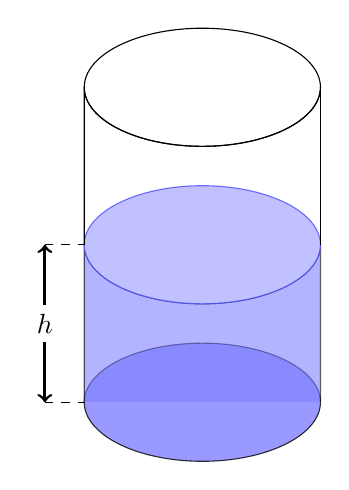
\begin{tikzpicture}
		\pgfmathsetmacro{\R}{1.5} 
		\pgfmathsetmacro{\H}{4} 
		 \pgfmathsetmacro{\h}{2}
		 \pgfmathsetmacro{\waterLevel}{\h}
		\pgfmathsetmacro{\nozzleY}{-0.2} 
		\pgfmathsetmacro{\nozzleX}{\R} 
		\draw[fill=blue!50,opacity=0.8] (0,0) ellipse ({\R} and {0.5*\R}); 
		\draw[fill=blue!50,opacity=0.6] ({-\R},0) -- ({-\R},\waterLevel) arc  (180:360:{\R} and {0.5*\R}) -- ({\R},\waterLevel) -- ({\R},0);
		\draw[blue!70,fill=blue!30,opacity=0.8] (0,\waterLevel) ellipse  ({\R} and {0.5*\R});
		\draw ({-\R},\waterLevel) --  ({-\R},\H) arc (180:360:{\R} and {0.5*\R});
		 \draw ({\R},\waterLevel) -- ({\R},\H);
		\draw (0,\H) ellipse ({\R}  and {0.5*\R});
		\draw[<->,line width=1pt]  ({-\R-0.5},0) -- node[pos=0.5,fill=white] {$h$}
			 ({-\R-0.5},\h);
		 \draw[dashed] ({-\R-0.5},0)--(-\R,0)
			({-\R-0.5},\h)--(-\R,\h); 
	\end{tikzpicture}
	} 
	 \loigiai{
		Theo đề bài, ta  có chiều cao bể $H=9$ m và bán kính đáy $R=2$ m.\\
		Thể tích ban đầu của bể $V_{\text{  bể}}=\pi R^2H=\pi 2^2\cdot 9=36\pi$ m$^3$.\\
		Tốc độ thoát nước $V'(t)=k(45-t)$  m$^3$/phút.\\
		Sau $15$ phút, độ cao mực nước trong  bể là $4$ m.\\
		$V(t)$ là thể tích chất lỏng đã thoát ra tại thời điểm $t$ (phút) sau khi  mở vòi.
		 Lấy nguyên hàm: \allowdisplaybreaks
		\begin{eqnarray*}
			V(t)&=&\displaystyle\int  V'(t)\mathrm{d}t = \displaystyle\int k(45-t)\mathrm{d}t \\
			&=&k\displaystyle\int  \left(45-t\right)\mathrm{d}t = k\left(\displaystyle\int 45\mathrm{d}t - \displaystyle\int t\mathrm{d}t\right)=k\left(45t-\dfrac{t^2}{2}\right)+C
		\end{eqnarray*}
		Biết tại thời điểm ban đầu ($t=0$) bể đầy nước  nên thể tích nước thoát ra là $V(0)=0$.\\
		 \[\Rightarrow V(0)=k\left(45\cdot 0-\dfrac{0^2}{2}\right)+C=0\Leftrightarrow C=0\Rightarrow V(t)=k\left(45t-\dfrac{t^2}{2}\right).\]
		Sau  $15$ phút, độ cao mực nước trong bể là $4$ m, vậy nước thoát ra là $9-4=5$ m.\\
		Thể tích nước còn lại sau $15$  phút là $V_{\text{ còn lại}}(15)=\pi R^2h(15)=\pi (2^2)(4)=16\pi$ m$^3$.\\
		Thể tích nước đã thoát ra sau $15$ phút là $V(15)=V_{\text{  bể}}-V_{\text{ còn lại}}=36\pi-16\pi=20\pi$ m$^3$.\\
		Thay $t=15$  và $V(15)=20\pi$ vào công thức $V(t)$:
		 \allowdisplaybreaks
		\begin{eqnarray*}
			&\Rightarrow& 20\pi =  k\left(45\cdot 15-\dfrac{15^2}{2}\right)\Leftrightarrow k\left(562{, }5\right)=20\pi \Leftrightarrow k=\dfrac{8\pi}{225} \\
			&\Rightarrow&  V(t)=\dfrac{8\pi}{225}\left(45t-\dfrac{t^2}{2}\right).
		\end{eqnarray*}
		 Ta tính
		 $V(42)=\dfrac{8\pi}{225}\left(45\cdot 42-\dfrac{42^2}{2}\right)=\dfrac{8\pi}{225}\left(1\,890-882\right)=\dfrac{8\,064\pi}{225}$ m$^3$.\\
		Vậy thể tích chất lỏng  còn lại trong bể là
		\[V_{\text{ còn lại}}=36\pi - V(42)=36\pi - \dfrac{8\,064\pi}{225}=\left(\dfrac{36\cdot 225-8\,064}{225}\right)\pi=\dfrac{4\pi}{25} \,\text{ m}^3 \] 
		Đổi $V_{\text{ còn lại}}=\dfrac{4\pi}{25}\cdot 1\,000 \text{ (lít)} \approx 502{,}6548$  lít.\\
		Làm tròn đến hàng đơn vị ta  được $V_{\text{ còn lại}} \approx 503 \text{ (lít)}$.
	} 
\end{bt}

% nguồn: Phan2_Lop_12_Dai_so_Chuong_4
\begin{bt}%[2D4V1-6]%[ma:49bcf3ed]
	\immini[thm]{Gọi $h(t)$ cm là mực nước ở một bồn chứa sau khi bơm nước vào bồn được $t$ giây. Biết rằng $h'(t)=k\cdot \sqrt[3]{t}$ và lúc đầu bồn không có nước. Sau $162$ giây, mực nước của bồn là $27$ cm. Biết bồn chứa nước cao $12{,}96$ m, hỏi sau bao nhiêu giây bồn chứa nước sẽ đầy?}{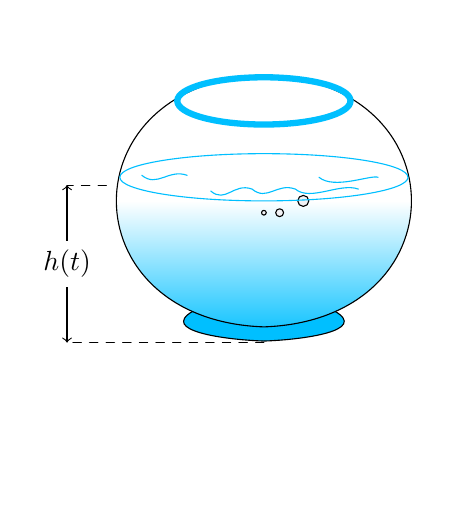
\begin{tikzpicture}[line join=round,line cap=round,scale=1,transform shape]
		 \definecolor{applegreen}{rgb}{0.55,0.71,0.0}
		 \definecolor{capri}{rgb}{0.0,0.75,1.0}
		\definecolor{amber}{rgb}{1.0,0.49,0.0} 
		 \definecolor{burntumber}{rgb}{0.54,0.2,0.14}
		 \definecolor{aliceblue}{rgb}{0.94,0.97,1.0}
		\definecolor{anti-flashwhite}{rgb}{0.95,0.95,0.96} 
		\clip (-3,-3) rectangle  (2,3);
		 \tikzset{be/.pic={
		\def\D{ 
			 (0,-.98)
			 ..controls +(178:.5) and +(-150:.5)..(-.9,-.6)--(.9,-.6)
			..controls +(-30:.5) and +(2:.5)..cycle; 
		 }
		 \fill[capri] \D;
		 \draw\D;
		 \def\N{
			 (0,2.4)
			..controls +(-178:2.5) and +(178:2.5)..(0,-.8) 
			..controls +(2:2.5) and +(-2:2.5)..cycle; 
		 }
		\fill[bottom color=capri!90,top color=white,middle  color=white] \N;
		 \draw\N;
		\draw[line width=.8mm,color=capri] (1.1,2.07)  arc (0:360:1.1 cm and 0.3cm);
		\draw[fill=anti-flashwhite] (0,.65) circle  (.03);
		\draw[fill=anti-flashwhite] (.2,.65) circle (.05); 
		 \draw[fill=anti-flashwhite] (.5,.8) circle (.07);
		\draw[capri] (1.83,1.1) arc  (0:360:1.83 cm and 0.3cm);
		\def\V{ 
			 (-.35,.74)
			..controls  +(120:.12) and +(40:.22)..(-.7,.72)--cycle
			(-.7,.32) 
			..controls  +(-170:.1) and +(10:.1)..(-.95,.3)
			..controls +(60:.1) and +(-140:.1)..(-.85,.45)--(-.65,.4)--cycle 
			(-.3,.32) 
			 ..controls +(-170:.1) and +(10:.1)..(-.45,.1)
			..controls  +(-40:.1) and +(-110:.1)..(-.1,.37)--cycle;
		 }
			 }}
		\tikzset{song/.pic={ 
		\def\S{ 
			 (-1.35,-2.15)
			 ..controls +(160:.5) and +(-40:.5)..(-2.5,-2.15)
			(3.5,-2.2) 
			..controls +(160:.2) and  +(-40:.5)..(2,-2.2)
			 (3,-2.5)
			..controls +(160:.5)  and +(-40:.5)..(1.4,-2.5)
			 ..controls +(160:.5) and +(-40:.5)..(.3,-2.5)
			..controls +(160:.5)  and +(-40:.5)..(-.75,-2.55);}
		\draw[capri]  \S;
			 }}
		 \path (0,0) pic[scale=1]{be}
			 (-.3,2.2) pic[scale=.5]{song};
		 \draw[<->] (-2.5,-1)--(-2.5,1) node[pos=0.5,fill=white]{$h (t)$};
		\draw[dashed]  (0,-1)--(-2.5,-1)
			 (-2,1)--(-2.5,1);
	\end{tikzpicture}
	} 
	\shortans{2954} 
	 \loigiai{
		Theo bài ta có: $h'(t)=k\cdot \sqrt[3]{t} \Rightarrow h(t)=\displaystyle\int k\cdot t^{\frac{1}{3}}\mathrm{\,d}t = k\cdot \dfrac{t^{\frac{4}{3}}}{\frac{4}{3}}+C = \dfrac{3}{4}k\cdot  t^{\frac{4}{3}}+C$.\\
		Tại $t=0 \Rightarrow h=0  \Leftrightarrow C=0\Rightarrow h(t)=\dfrac{3}{4}k\cdot t^{\frac{4}{3}}$.\\
		Tại $t=162 \Rightarrow  h=27$ cm.\\
		Ta đổi $12{,}96$ m$=  1\,296$ cm (chiều cao bồn).\\
		Áp dụng  điều kiện $h(162)=27$ cm, ta được $\dfrac{3}{4}k\cdot 162^{\frac{4}{3}}=27$.\\
		Để bồn đầy, ta cần $h(t)=1\,296$ cm. Ta có tỉ lệ 
		\allowdisplaybreaks 
		\begin{eqnarray*}
			 &&\dfrac{h(t)}{h(162)}=\dfrac{\dfrac{3}{4}k\cdot t^{\frac{4}{3}}}{\dfrac{3}{4}k\cdot 162^{\frac{4}{3}}}=\dfrac{1296}{27} \\
			&&\Leftrightarrow \left(\dfrac{t}{162}\right)^{\frac{4}{3}} = \dfrac{1296}{27}=48\Leftrightarrow \dfrac{t}{162} = 48^{\frac{3}{4}}  \\
			&&\Leftrightarrow t =162 \cdot 48^{\frac{3}{4}} \approx 2953{,}78  \text{ (giây)}\Leftrightarrow t \approx 2954 \text{ (giây)}
		\end{eqnarray*}
	} 
\end{bt}

% nguồn: Phan2_Lop_12_Dai_so_Chuong_4
\begin{bt}%[2D4V1-6]%[ma:8608d946]
	Số dân của một thị trấn sau $t$ năm kể từ năm 1990 được ước tính theo một hàm số theo thời gian $f(t)$ ($f(t)$ được tính bằng nghìn người). Biết rằng $f'(t)=\dfrac{34}{t^2+4t+4}$  (nghìn người/năm) biểu thị tốc độ tăng dân số của thị trấn. Số dân của thị trấn đó vào năm $2\,035$ là bao nhiêu (kết quả lấy chính xác đến hàng phần chục) biết dân số của thị trấn đó năm 1990 là $3$ nghìn người ?
	\shortans{19,3} 
	\loigiai{ 
		Ta có $f'(t)=\dfrac{34}{t^2+4t+4}=\dfrac{34}{(t+2)^2}\Rightarrow  f(t)=-\dfrac{34}{t+2}+C$.\\
		Chọn mốc thời gian là năm  1990.\\
		Dân số  của thị trấn đó năm 1990 là $3$ nghìn người nên ta có $f(0)=3$.\\
		Khi đó $-\dfrac{34}{2}+C=3\Leftrightarrow C=20$ nên $f(t)=-\dfrac{34}{t+2}+20$.\\ 
		Từ năm 1990 đến năm 2035 là $45$ năm nên dân số của thị trấn năm 2035  là
		\[f(45)=-\dfrac{34}{47}+20=\dfrac{906}{47}\approx 19{,}3\text{  (nghìn người).}\]
	} 
\end{bt}

% nguồn: Phan2_Lop_12_Dai_so_Chuong_4
\begin{bt}%[2D4V1-6]%[ma:bead7e26]
	Một viên đạn được bắn lên trời với vận tốc là $72$ m/s bắt đầu từ độ cao $2$ m. Hãy xác định chiều cao của viên đạn sau thời gian $5$ giây kể từ lúc bắn, biết gia tốc trọng trường là $9{,}8$ m/s$^2$ (kết quả làm tròn đến  hàng đơn vị).
	 \shortans{240}
	 \loigiai{
		Vận tốc của viên đạn  tại thời điểm $t$ là
		 $$v(t) = \displaystyle\int -9{,}8\,\mathrm{d}t = -9{,}8t + C_1.$$
		Vì  $v(0) = 72$ nên $C_1 = 72 \Rightarrow v(t) = -9{,}8t + 72$.\\
		Độ cao  của viên đạn tại thời điểm $t$ là
		$$s(t) =  \displaystyle\int v(t)\,\mathrm{d}t = \displaystyle\int (-9{,}8t + 72)\,\mathrm{d}t = -4{,}9t^2 + 72t + C_2.$$
		Vì $s(0) = 2$ nên $C_2 =  2 \Rightarrow s(t) = -4{,}9t^2 + 72t + 2$.\\
		Vậy sau $5$ giây kể từ  lúc bắn, viên đạn ở độ cao:
		 $$s(5) = -4{,}9 \cdot 25 + 72 \cdot 5 + 2 = -122{,}5 + 360 + 2 = 239{,}5\approx 240.$$
		Chiều  cao của viên đạn sau thời gian $5$ giây kể từ lúc bắn là khoảng $240$ m.
	 }
\end{bt}

% nguồn: Phan2_Lop_12_Dai_so_Chuong_4
\begin{bt}%[2D4V1-6]%[ma:fb8297ee]
	\immini{Một vật chuyển động với hàm số gia tốc là $a(t)$. Biết rằng đồ thị hàm số $a(t)$ trên đoạn $[0;6]$ được cho như hình  dưới đây và vận tốc tại thời điểm $t=0$ là $v(0)=1$ (m/s). Tại thời điểm $t=6$ giây, vận tốc của vật là bao nhiêu? (làm tròn kết quả đến chữ số thập phân thứ nhất).
	}{\begin{tikzpicture}[scale=0.7,font=\footnotesize,yscale=0.8]
		\begin{axis}[
				width=11cm,height=6cm, 
				axis  lines=middle,
				xlabel={$x$}, 
				ylabel={$y$}, 
				 xmin=-0.5,xmax=7,
				 ymin=-0.1,ymax=2,
				xtick={0,2,6}, 
				 xticklabels={0,2,6},
				ytick={sqrt  (2),sqrt (3)},
				 yticklabels={$\sqrt2$,$\sqrt3$},
				domain=0:6, 
				 samples=2,
				every axis x label/.style={at={(axis description  cs:0.98,0.02)},anchor=north east},
				every axis y label/.style={at={(axis description  cs:0.02,0.95)},anchor=south west},
				 clip=false]
			\addplot[domain=0:2] {(sqrt (2)/2) * x} node[pos=0.45,above left] {}; 
			\addplot[domain=2:6] {((sqrt (3)-sqrt (2))/4) * x  + (3*sqrt (2)-sqrt (3))/2}
				node[pos=0.85,above]  {$a (t)$};
			 \draw[densely dashed] (axis cs:0,{sqrt (2)}) -- (axis cs:6,{sqrt (2)});
			\draw[densely dashed] (axis cs:0,{sqrt  (3)}) -- (axis cs:6,{sqrt (3)});
			\draw[densely dashed] (axis cs:2,0) --  (axis cs:2,{sqrt (2)});
			\draw[densely dashed] (axis cs:6,0)  -- (axis cs:6,{sqrt (3)});
			\addplot[only marks,mark=*,mark  options={scale=1.1}] coordinates {(2,{sqrt (2)})
				 (6,{sqrt (3)})};
			\node[anchor=west] at (axis  cs:2,{sqrt (2)}) {};
			\node[anchor=west] at (axis  cs:6,{sqrt (3)}) {};
			\node[anchor=north  east] at (axis cs:0,0) {0};
		\end{axis}
	\end{tikzpicture}
	} 
	\shortans{8,7} 
	 \loigiai{
		Từ đồ thị  ta có
		 $$
		 a(t) =
		 \heva{
		&\dfrac{\sqrt{2}}{2}t, &  0 \le t \le 2,\\[6pt]
		 &\dfrac{\sqrt{3}-\sqrt{2}}{4}t + \dfrac{3\sqrt{2}-\sqrt{3}}{2}, & 2 \le t \le 6.
		} 
		 $$
		Vì  $v(0)=1$, nên
		 $$
		v(t) = \int  a(t)\,\mathrm{d}t =
		 \heva{
		&\dfrac{\sqrt{2}}{4}t^2  + 1, & 0 \le t \le 2,\\[6pt]
		&\dfrac{\sqrt{3}-\sqrt{2}}{8}t^2  + \dfrac{3\sqrt{2}-\sqrt{3}}{2}t + C, & 2 \le t \le 6.
		 }
		$$ 
		 Do vận tốc là hàm số liên tục nên
		$$ 
		\lim_{t \to 2^-}  v(t) = \lim_{t \to 2^+} v(t)
		\Rightarrow \sqrt{2} + 1 = \dfrac{\sqrt{3}-\sqrt{2}}{2} \cdot 2^2 +  3\sqrt{2}-\sqrt{3} + C
		 \Rightarrow C = \dfrac{\sqrt{3}-3\sqrt{2}+2}{2}.
		 $$
		Suy ra 
		 $$
		v(6) = 1 + 3\sqrt{2} + 2\sqrt{3}  \approx 8{,}7 \text{ (m/s)}.
	 $$}
\end{bt}

% nguồn: Phan2_Lop_12_Dai_so_Chuong_4
\begin{bt}%[2D4V1-6]%[ma:c375197b]
	\immini[thm]{Một bể nước hình hộp chữ nhật cao $1$ m và có đáy là hình vuông cạnh $2$ m. Ban đầu bể đầy nước. Người ta mở một cái vòi ở đáy, nước chảy ra với tốc độ tỷ lệ thuận với căn bậc hai của độ cao của nước tại bất kì thời điểm nào. Giả sử độ cao của nước trong bể tại thời điểm $t$ là $h(t)$ và $V(t)$ là thể tích của nước hiện tại sau $t$ phút mở vòi thì ta có $V'(t)=k\cdot \sqrt{h(t)} $ với $ (k\in \mathbb{R})$.\\ 
	Biết rằng,  mực nước giảm $19$ cm sau $2$ phút, hỏi sau bao nhiêu phút thì bể cạn nước?
	 \shortans{20}
	}{ 
	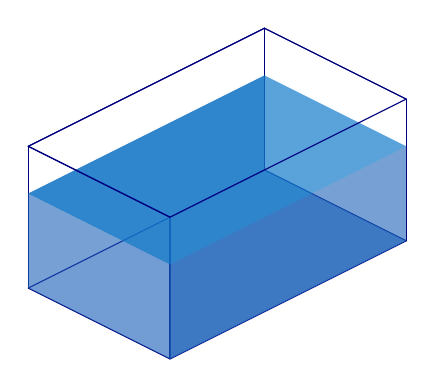
\begin{tikzpicture}[
				 x={(1cm,0.5cm)},
				 y={(-1cm,0.5cm)},
				 z={(0cm,1cm)},
				scale=0.6, 
				line cap=round,line  join=round]
			 \def\len{5}
			 \def\wid{3}
			 \def\hgt{3}
			\def\waterhgt{2} 
			\fill[blue!10,opacity=0.5] (0,0,0) -- (\len,0,0) -- (\len,\wid,0) -- (0,\wid,0)  -- cycle;
			 \draw[blue!50!black,thin] (0,0,0) -- (\len,0,0) -- (\len,\wid,0) -- (0,\wid,0) -- cycle;
			\draw[blue!50!black] (0,0,0) -- (0,0,\hgt); 
			\draw[blue!50!black]  (0,\wid,0) -- (0,\wid,\hgt);
			 \draw[blue!50!black] (\len,0,0) -- (\len,0,\hgt);
			\draw[blue!50!black]  (\len,\wid,0) -- (\len,\wid,\hgt);
			\fill[cyan!40!blue,opacity=0.6] (0,0,0) -- (\len,0,0)  -- (\len,\wid,0) -- (0,\wid,0) -- cycle;
			\fill[cyan!40!blue,opacity=0.6] (0,0,0) -- (\len,0,0)  -- (\len,0,\waterhgt) -- (0,0,\waterhgt) -- cycle;
			\fill[cyan!40!blue,opacity=0.6] (0,\wid,0)  -- (\len,\wid,0) -- (\len,\wid,\waterhgt) -- (0,\wid,\waterhgt) -- cycle;
			 \fill[cyan!60!blue,opacity=0.7] (0,0,\waterhgt) -- (\len,0,\waterhgt) -- (\len,\wid,\waterhgt) -- (0,\wid,\waterhgt) -- cycle;
			\draw[blue!50!black] (0,0,\hgt) -- (\len,0,\hgt) -- (\len,\wid,\hgt)  -- (0,\wid,\hgt) -- cycle;
			\draw[blue!50!black] (0,0,\hgt) -- (0,\wid,\hgt); 
			\draw[blue!50!black]  (\len,0,\hgt) -- (\len,\wid,\hgt);
			\draw[blue!50!black] (0,\wid,\hgt)  -- (\len,\wid,\hgt);
		\end{tikzpicture}
	 }
	 \loigiai{
		Vì bể nước có dạng hình hộp chữ nhật có chiều cao $h(t)$ và  có đáy luôn là hình vuông cạnh $2$ m nên thể tích của hình hộp tại thời điểm $t$ là $V(t)=2^2h(t)=4h(t)$.\\
		Ta có 
		\begin{eqnarray*}
			V'(t)=4h'(t) &\Leftrightarrow& V'(t)=k\cdot \sqrt{h(t)}  \Leftrightarrow 4h'(t)=k\cdot \sqrt{h(t)} \\
			&\Leftrightarrow& \dfrac{h'(t)}{\sqrt{h(t)}}=\dfrac{k}{4} \Leftrightarrow \left(2\sqrt{h(t)}\right)'=\dfrac{k}{4} \Leftrightarrow \left(\sqrt{h(t)}\right)'=\dfrac{k}{8} 
		\end{eqnarray*}
		 Nguyên hàm $2$ vế, ta được $\sqrt{h(t)}=\displaystyle\int \dfrac{k}{8}\mathrm{\,d}t=\dfrac{k}{8}t+C$.\\
		 Ta có độ cao của nước tại thời điểm ban đầu bằng $1$m tức $h(0)=1$ nên ta có
		\[\sqrt{h(0)}=\sqrt{1}=\dfrac{k}{8}\cdot 0+C  \Leftrightarrow C=1\Rightarrow \sqrt{h(t)}=\dfrac{k}{8}t+1.\]
		Lại có, sau $2$ phút, mực nước giảm $19$cm (hay $0{,}19$m) thì độ  cao của nước trong bể bằng \break$h=1-0{,}19=0{,}81$ nên ta có
		\[h(2)=0{,}81\Leftrightarrow \sqrt{h(2)}=\sqrt{0{,}81}=\dfrac{k}{8}\cdot 2+1 \Leftrightarrow 0{,}9=\dfrac{k}{4}+1 \Leftrightarrow \dfrac{k}{4}=-0{,}1 \Leftrightarrow k=-0{,}4.\] 
		Vậy  $\sqrt{h(t)}=\dfrac{-0{,}4}{8}t+1=-0{,}05t+1$.\\
		Bể cạn nước khi chiều cao của nước trong bể  bằng $0$ hay $h(t)=0$.\\
		Suy ra $\sqrt{h(t)}=0 \Rightarrow  -0{,}05t+1=0 \Leftrightarrow t=20$.\\
		 Vậy sau $20$ phút thì bể cạn nước.
	} 
\end{bt}

% nguồn: Phan2_Lop_12_Dai_so_Chuong_4
\begin{bt}%[2D4V1-6]%[ma:b3b95a5c]
	\immini{Một viên đạn được bắn thẳng đứng lên từ mặt đất với vận tốc tại thời điểm $t=0$ là $v(t) = 180 - 9{,}8t$ (m/s). Tìm độ cao cực đại của viên đạn (tính từ mặt đất) khi nó đạt tới điểm cao  nhất. (Làm tròn kết quả đến hàng đơn vị.)
	}{	\begin{tikzpicture}[scale=0.7]
		\shade[left  color=yellow!60!orange,right color=yellow!80!brown,shading angle=0]
			 (0,0) rectangle (0.6,1.6);
		\shade[top color=brown!70!red,bottom  color=yellow!60!orange,shading angle=90]
		(0,1.6) arc[start angle=180,end angle=0,x radius=0.3,y radius=0.4]
		-- (0.6,1.6) --  (0,1.6) -- cycle;
	 \fill[yellow!80!brown!80!black] (0,0) rectangle (0.6,-0.2);
	\draw[line  width=1pt,densely dashed] (0.3,-0.2) -- (0.3,-1.2);
	\draw[-{Latex[length=3mm,width=2mm]}]  (1,-.5) -- (1,1.0);
\end{tikzpicture}
	} 
	 \shortans{1653}
	 \loigiai{
		Độ cao $h(t)$ của viên đạn 
		$$h(t) = \int v(t)\,\mathrm{d}t = \int (180 - 9{,}8t)\,\mathrm{d}t  = 180t - 4{,}9t^2 + C.$$
		Tại $t=0$,  $h(0)=0 \Rightarrow C=0.$
		 Vậy
		$$h(t) =  180t - 4{,}9t^2.$$
		Khi  đạt độ cao cực đại
		$$v(t) = 0 \Rightarrow 180 - 9{,}8t = 0  \Rightarrow t_{\max} = \frac{180}{9{,}8}.$$
		 Suy ra
		 $$
		h_{\max} = 180t_{\max} -  4{,}9t_{\max}^2
		=  180\!\left(\frac{180}{9{,}8}\right) - 4{,}9\!\left(\frac{180}{9{,}8}\right)^2
		\approx 1\, 653\,(\text{m}). 
	$$} 
\end{bt}

% nguồn: Phan2_Lop_12_Dai_so_Chuong_4
\begin{bt}%[2D4V1-6]%[ma:49f38b36]
	Một xe ô tô sau khi chờ hết đèn đỏ đã bắt đầu chuyển động với  vận tốc được biểu thị bằng đồ thị là đường cong parabol như hình bên dưới. Biết rằng sau $5$~(phút) thì xe đạt đến vận tốc cao nhất $1000$~(m/ phút) và bắt đầu giảm vận tốc, đi được $6$~(phút) thì xe chuyển động đều.
	\begin{center}
		\begin{tikzpicture}[scale=.5,font=\footnotesize,line join=round,line cap=round,>=stealth]
				 \draw[->] (0,0) -- (11,0) node[below right] {$t$};
				\draw[->] (0,0) --  (0,12) node[left] {$v$};
				 \node[below left] at (0,0) {$O$};
				\foreach \x in {5,6,10}{ 
					 \draw (\x,0.1) -- (\x,-0.1);
					 \node[below] at (\x,-0.1) {$\x$};
				 }
				\foreach \y  in {0,10}{
					 \draw (0.1,\y) -- (-0.1,\y);
				} 
				\node[left] at  (0,10) {$1\,000$};
				\draw[domain=0:6,samples=100,smooth,variable=\t] 
					plot  ({\t},{(-40)*(\t)^2/100 + (400)*\t/100});
				\draw (6,9.6)  -- (10,9.6);
				\draw[dashed] (5,0)  -- (5,10);
				\draw[dashed] (6,0) --  (6,10);
				 \draw[dashed] (10,0) -- (10,10);
				 \draw[dashed] (0,10) -- (10,10);
			\end{tikzpicture}
	\end{center}
	Hỏi  quãng đường xe đã đi được trong khoảng $10$ phút đầu tiên là bao nhiêu?
	\shortans{8160} 
	\loigiai{ 
		Dựa vào đồ thị, phương trình vận tốc là $v(t)=-40t^2+400t$ với $t\in [0;6]$ và $v=960$ với  $t>6$.\\
		Trong khoảng $6$ phút đầu phương trình  quãng đường là
		\[S(t)=\displaystyle\int{\left(-40t^2+400t\right)}\mathrm{\,d}t=-\dfrac{40}{3}t^3+200t^2+C.\] 
		Tại thời  điểm xe ô tô xuất phát ta có $t_0=0$ và $S(t_0)=0$.\\
		Suy ra $C=0$ nên phương  trình quãng đường là $S(t)=-\dfrac{40}{3}t^3+200t^2$.\\
		Trong khoảng $6$  phút đầu ô tô đi được quãng đường là $S(6)=4\,320~\mathrm{m}$ và $4$ phút tiếp theo ô tô đi được quãng đường là $960\cdot4=3\,840~\mathrm{m}$.\\
		Vậy quãng đường ô tô  đi được trong $10$ phút đầu là $4\,320+3\,840=8\,160~\mathrm{m}$.
	 }
\end{bt}

% nguồn: Phan2_Lop_12_Dai_so_Chuong_4
\begin{bt}%[2D4V1-6]%[ma:08c8a4c2]
	Tốc độ phát triển của số lượng vi khuẩn trong hồ bơi được mô hình bởi hàm số $B'(t)=\dfrac{1\,000}{\left(1+0{,}3t\right)^2}$ với $t\ge 0$, trong đó $B(t)$ là số lượng vi khuẩn trên mỗi ml nước tại ngày thứ $t$. Số lượng vi khuẩn ban đầu là $500$ con trên mỗi ml nước. Biết rằng mức độ an toàn cho người sử dụng hồ bơi  là số vi khuẩn phải dưới $3\,000$ con trên mỗi ml nước. Hỏi sau bao nhiêu ngày thì người ta phải xử lí và thay nước mới cho hồ bơi.
	\shortans{10} 
	 \loigiai{
		 Số lượng vi khuẩn tại thời điểm $t$ là
		$$ 
		B(t) = \displaystyle\int B'(t)\,\mathrm{d}t  = \displaystyle\int \dfrac{1\,000}{(1 + 0{,}3t)^2} \,\mathrm{d}t = 1\,000 \displaystyle\int (1 + 0{,}3t)^{-2} \,\mathrm{d}t.
		$$ 
		Đặt $u =  1 + 0{,}3t \Rightarrow \mathrm{d}u = 0{,}3\,\mathrm{d}t \Rightarrow \mathrm{d}t = \dfrac{1}{0{,}3}\mathrm{d}u$, nên
		$$ 
		B(t)  = 1\,000 \cdot \dfrac{1}{0{,}3} \cdot \displaystyle\int u^{-2} \,\mathrm{d}u = -\dfrac{1\,000}{0{,}3(1 + 0{,}3t)} + C.
		$$ 
		 Ta có $B(0) = 500 \Rightarrow -\dfrac{1\,000}{0{,}3 \cdot 1} + C = 500 \Rightarrow C = 500 + \dfrac{1\,000}{0{,}3} = \dfrac{11\,500}{3}$.\\
		 Vậy
		 $$
		B(t)  = -\dfrac{1\,000}{0{,}3(1 + 0{,}3t)} + \dfrac{11\,500}{3}.
		 $$
		 Để $B(t) < 3\,000$ (an toàn) ta giải
		 $$
		-\dfrac{1\,000}{0{,}3(1 + 0{,}3t)} + \dfrac{11\,500}{3} < 3\,000 \Rightarrow -\dfrac{1\,000}{0{,}3(1 + 0{,}3t)} < -\dfrac{2\,500}{3} \Rightarrow 1  + 0{,}3t < 4 \Rightarrow t < 10.
		$$ 
		Vậy sau $10$ ngày thì hồ bơi  không còn an toàn và cần xử lý.
	 }
\end{bt}

% nguồn: Phan2_Lop_12_Dai_so_Chuong_4
\begin{bt}%[2D4V1-6]%[ma:1d03dedb]
	Gọi $h(t)$ là chiều cao của cây keo (tính theo mét) sau khi trồng $t$ năm. Biết rằng năm đầu tiên cây cao $1{,}5~\mathrm{m}$, trong những năm tiếp theo. Cây phát triển với tốc độ $h'(t)=\dfrac{1}{\sqrt[4]t}$ (mét /năm). Hỏi sau bao nhiêu  năm cây cao được $3~\mathrm{m} $?
	 \shortans{2,73}
	\loigiai{ 
		Ta  có $h'(t)=\dfrac{1}{\sqrt[4]t}$ $\Rightarrow h(t)=\displaystyle\int{\frac{1}{\sqrt[4]t}}\mathrm{\,d}t=\displaystyle\int{{t^{-\frac{1}{4}}}}\mathrm{\,d}t=\dfrac{{t^{-\frac{1}{4}+1}}}{^{-\frac{1}{4}+1}}+C=\dfrac{4}{3}\sqrt[4]{t^3}+C$ $\Rightarrow h(t)=\dfrac{4}{3}\sqrt[4]{t^3}+C$.\\
		Năm đầu tiên cây  cao $1~\mathrm{m}$ nên $h(1)=1,5\Leftrightarrow 1{,}5=\dfrac{4}{3}\sqrt[4]1+C\Rightarrow C=\dfrac{1}{6}$ $\Rightarrow h(t)=\dfrac{4}{3}\sqrt[4]{{t^3}}+\dfrac{1}{6}$.\\
		 Vậy cây cao được $3~\mathrm{m} $ nên $h(t)=3\Leftrightarrow \dfrac{4}{3}\sqrt[4]{t^3}+\dfrac{1}{6}=3\Leftrightarrow \sqrt[4]{t^3}=\dfrac{17}{8}\Rightarrow t\approx 2{,}73$.
	 }
\end{bt}

% nguồn: Phan2_Lop_12_Dai_so_Chuong_4
\begin{bt}%[2D4V1-6]%[ma:8ac36390]
	Người ta truyền nhiệt cho một bình nuôi cấy vi sinh vật từ $1^\circ C$. Tốc độ tăng nhiệt độ của bình tại thời điểm t phút $(0\le t\le 5)$ được cho bởi hàm số $f(t)=3t^2 (^\circ C$/phút). Biết rằng nhiệt độ của bình đó tại thời điểm $t$ là một nguyên hàm của hàm số $f(t)$, tìm nhiệt độ của bình  tại thời điểm $ 3$ phút kể từ khi truyền nhiệt. (Kết quả để theo đơn vị $^\circ C$).
	\shortans{28} 
	\loigiai{ 
		Gọi $ T(t)$ là nhiệt  độ của bình tại thời điểm $t$ phút.\\
		Ta có $  T(t)=\displaystyle\int f(t)\mathrm{d\,}t=\displaystyle\int{3t^2\mathrm{d\,}t}=t^3+C$.\\
		Vì người ta truyền nhiệt cho một bình nuôi  cấy vi sinh vật từ $1^{\circ}C$ nên
		$$ T(0)=1^{\circ}\Rightarrow C=1\Rightarrow T(t)=t^3+1.$$ 
	Vậy nhiệt độ của bình tại thời điểm $3$ phút kể từ  khi truyền nhiệt là $ T(3)=3^3+1=28\,(^{\circ}C)$.}
\end{bt}

% nguồn: Phan2_Lop_12_Dai_so_Chuong_4
\begin{bt}%[2D4V1-6]%[ma:2f07fc32]
	Một  viên đạn được bắn lên theo phương thẳng đứng từ mặt đất. Giả sử tại thời điểm $t$ giây (coi là thời điểm viên đạn được bắn lên), vận tốc của nó được cho bởi $v(t)=24{,}5-9{,}8t~\mathrm{m/s}$. Tính quãng đường (mét) viên đạn đi sau $2$ giây đầu.
	 \shortans{29,4}
	\loigiai{ 
		Quãng đường viên đạn đi  được là
		 $s(t) =\displaystyle\int\left(24{,}5-9{,}8t\right)\,\mathrm{d}t=24{,}5t-4{,}9t^2+C$.\\
		Thay $t=0\Rightarrow  s(0)=0\Rightarrow C= 0$.\\
		Suy ra  $s(t)=24{,}5t-4{,}9t^2$.\\
		Vậy sau $2$ giây đầu  quãng đường viên đạn đi là $s(2)=24{,}5\cdot2-4{,}9\cdot2^2=29{,}4~\mathrm{m} $.
	 }
\end{bt}

% nguồn: Phan2_Lop_12_Dai_so_Chuong_4
\begin{bt}%[2D4V1-6]%[ma:5f9eb279]
	Một vật đang chuyển động với vận tốc $6$ m/s thì tăng tốc với gia tốc $a(t)=\dfrac{3}{t+1}$ m/s$^2$, trong đó $t$ là khoảng thời gian (giây) kể từ lúc bắt đầu tăng tốc. Hỏi vận tốc của vật sau $10$ giây gần nhất với kết quả nào  sau đây?
	 \shortans{13}
	 \loigiai{
		Vận  tốc tại thời điểm $t$ là
		$$v(t) = \displaystyle\int a(t)\,\mathrm{d}t = \displaystyle\int \dfrac{3}{t+1}\,\mathrm{d}t  = 3\ln|t+1| + C.$$
		Tại thời điểm bắt đầu tăng tốc $(t=0)$ thì $v(0) = 6$ m/s nên 
		$$3\ln 1 + C = 6  \Rightarrow C = 6.$$
		 Suy ra
		$$v(t) = 3\ln(t+1)  + 6.$$
		Tại $t = 10$: 
		$$v(10) = 3\ln 11 + 6 \approx 3 \cdot 2{,}398 + 6 \approx 7{,}194 +  6 = 13{,}194.$$
		Vậy vận tốc gần đúng  là $13$ m/s.
	} 
\end{bt}

% nguồn: Phan2_Lop_12_Dai_so_Chuong_4
\begin{bt}%[2D4V1-6]%[ma:2e73f0f8]
	Một bác thợ xây bơm nước vào bể chứa nước. Gọi $h(t)$ là thể tích nước bơm được sau $t$ giây. Cho $h'(t)=6at^2+2bt$ và ban đầu bể không có nước. Sau $3$ giây thì thể tích nước trong bể là $90$ m$^3$ và sau 6 giây thì thể tích nước trong bể là $504$ m$^3$. Tính thể tích nước trong bể sau khi bơm được $9$  giây.
	 \shortans{1,458}
	\loigiai{ 
		Ta có $h(t)=\displaystyle\int (6at^2 + 2bt) \mathrm{\,d}t = 2at^3 + bt^2 + c$.\\ 
		Ban đầu bể không  có nước nên $h(0)=0 \Rightarrow c=0$.\\
		Thay vào các điều kiện còn  lại:
		\begin{itemize}
			\item $h(3)=90 \Rightarrow 2a\cdot 27 + b\cdot 9 = 90 \Rightarrow 54a +  9b = 90$.
			\item $h(6)=504 \Rightarrow 2a\cdot 216 + b\cdot 36 = 504 \Rightarrow 432a + 36b =  504$.
		\end{itemize}
		Giải hệ: $\heva{&54a + 9b = 90\\& 432a + 36b = 504} \Rightarrow \heva{&a  = \dfrac{2}{3}\\& b = 6.}$\\
		Vậy $h(t) =  \dfrac{4}{3}t^3 + 6t^2 \Rightarrow h(9) = \dfrac{4}{3}\cdot 729 + 6\cdot 81 = 972 + 486 = 1\,458$.\\
		Thể tích nước trong bể  sau $9$ giây là $1\,458$ m$^3$.
	 }
\end{bt}

% nguồn: Phan2_Lop_12_Dai_so_Chuong_4
\begin{bt}%[2D4V1-6]%[ma:0349ad45]
	Cường độ dòng điện trong một dây dẫn tại thời điểm $t~\text{ (giây)}$ là $I(t)=Q'(t)=3t^2-6t+5$. Với $Q(t)$ là  điện lượng truyền trong dây dẫn tại thời điểm $t$. Biết khi $t=1$ giây, điện lượng truyền trong dây dẫn là $Q(1)=4$. Tính điện lượng truyền trong dây dẫn khi $t=3$ giây.
	\shortans{16} 
	\loigiai{ 
		Ta có 
		\[Q(t)=\displaystyle\int{Q'(t)}\text{ d}t=\displaystyle\int{\left(3t^2-6t+5\right)}\text{ d}t={t^3}-3{t^2}+5t+C.\] 
		Do $Q(1)=4$  nên
		\[1^3-{{3\cdot1}^2}+5\cdot1+C=4\Rightarrow  C=1.\]
		Như vậy 
		\[Q(t)={t^3}-3{t^2}+5t+1\] 
		nên 
		\[Q(3)=3^3-{{3\cdot3}^2}+5\cdot3+1=16.\] 
	} 
\end{bt}

% nguồn: Phan2_Lop_12_Dai_so_Chuong_4
\begin{bt}%[2D4V1-6]%[ma:b956da42]
	Một bác thợ  xây bơm nước vào bể chứa nước. Gọi $h(t)$ là thể tích nước bơm được sau $t$ giây. Cho $h'(t)=3at^2+bt$ (m$^3$/s) và ban đầu bể không có nước. Sau $5$ giây thì thể tích nước trong bể là $150$ m$^3$. Sau $10$ giây thì thể tích nước trong bể là $1\,100$ m$^3$. Hỏi thể tích nước trong bể sau khi bơm được $20$ giây.
	\shortans{8400} 
	 \loigiai{
		Ta có $h'(t) =  3at^2 + bt$ nên
		$$ 
		h(t) = \displaystyle\int (3at^2 + bt)\,\mathrm{d}t = at^3  + \dfrac{1}{2}bt^2 + C.
		 $$
		Vì ban đầu bể không có nước  nên $h(0) = 0 \Rightarrow C = 0$, do đó
		$h(t) = at^3 +  \dfrac{1}{2}bt^2$.
		Ta có 
		\begin{itemize}
			\item  $h(5) = 125a + \dfrac{25}{2}b = 150$.
			 \item $h(10) = 1\,000a + 50b = 1\,100$.
		\end{itemize}
		Giải hệ phương  trình
		$$ 
		\heva{ 
		&125a + \dfrac{25}{2}b = 150  \\
		 &1\,000a + 50b = 1\,100
		} 
		 \Rightarrow \heva{&a=1\\&b=2.}
		 $$
		 Vậy
		$$ 
		h(t) = t^3 + t^2 \Rightarrow h(20) = 20^3 + 20^2 = 8\,000 + 400 =  8\,400.
		$$ 
		Thể tích nước trong  bể sau khi bơm được $20$ giây là $8\,400$ m$^3$.
	} 
\end{bt}

% nguồn: Phan2_Lop_12_Dai_so_Chuong_4
\begin{bt}%[2D4V1-6]%[ma:a5029735]
	Một chiếc cốc chứa nước ở $95$\,$^\circ$C được đặt trong phòng có nhiệt độ $20$\,$^\circ$C. Tốc độ giảm nhiệt độ sau $t$ phút là $T'(t)=-\dfrac{3}{2}\mathrm{e}^{-\tfrac{t}{50}}$ ($^\circ$C/phút). Tính nhiệt độ của nước tại thời điểm $t=30$ phút (kết quả làm tròn đến hàng  phần chục).
	\shortans{61,2} 
	 \loigiai{
		Ta có nhiệt độ của  nước trong cốc sau $t$ phút là
		\[T(t)=\displaystyle\int  T'(t)\mathrm{\,d}t=-\dfrac{3}{2}\displaystyle\int \mathrm{e}^{{-\tfrac{t}{50}}}\mathrm{\,d}t=75\mathrm{e}^{-\tfrac{t}{50}}+C. \]
		Với $T(0)=95$, ta  có $75+C=95 \Rightarrow C=20$.\\
		Suy ra  $T(t)=75\mathrm{e}^{{-\tfrac{t}{50}}}+20$.\\
		Vậy $T(30)=75\mathrm{e}^{{-\tfrac{30}{50}}}+20 \approx  61{,}2$.
	} 
\end{bt}

% nguồn: Phan2_Lop_12_Dai_so_Chuong_4
\begin{bt}%[2D4V1-6]%[ma:6f0a9353]
	Một vật được ném lên từ độ cao $300$\,m với vận tốc được cho bởi công thức \linebreak $v(t)=-9{,}81t+29{,}43$\,(m/s) (\textit{Nguồn: R. Larson  and B. Edwards, Calculus 10e, Cengane}). Gọi $h(t)$ (m) là độ cao của vật tại thời điểm $t$\,(s). Sau bao lâu kể từ khi bắt đầu được ném lên thì vật đó chạm đất (làm tròn kết quả đến hàng phần chục giây)?
	 \shortans{11,4}\loigiai{
		Ta có $h(t)=\displaystyle\int v(t) \mathrm{\,d} t=\displaystyle\int(-9{,}81\cdot t+29{,}43) \mathrm{\,d}  t=-\dfrac{9{,}81}{2} t^2+29{,}43\cdot t+C$.\\
		Vì vật được ném lên từ độ cao  $300$\,m nên $h(0)=300$. Suy ra $C=300$.\\
		Vậy $h(t)=-\dfrac{9{,}81}{2} t^2+29{,}43  t+300$.\\
		Khi vật  bắt đầu chạm đất ứng với $h(t)=0$.\\
		Nên ta có $-\dfrac{9{,}81}{2} t^2+29{,}43\cdot t+300=0 \Leftrightarrow t \approx 11{,}4$ hoặc  $t \approx-5{,}4$.\\
		 Do $t>0$ nên $t \approx 11{,}4$ giây.
	} 
\end{bt}

% nguồn: Phan2_Lop_12_Dai_so_Chuong_4
\begin{bt}%[2D4V1-6]%[ma:1eb6f9e5]
	Người ta quan sát một quần thể vi khuẩn đang tăng trưởng, ban đầu gồm $500$ vi khuẩn. Sau một ngày và sau bốn ngày kể từ khi bắt đầu quan sát, số lượng vi khuẩn của quần thể đó tương ứng là $600$ vi khuẩn, $1\,300$ vi khuẩn. Gọi $P(t)$ là số lượng vi khuẩn của quần thể đó tại thời điểm $t$ ngày kể từ khi bắt đầu quan sát, $0 \le t \le 10$. Người ta ước tính tốc độ tăng trưởng của quần thể vi khuẩn đó được mô  tả bởi $P'(t) = at + b\sqrt{t}$ (vi khuẩn/ngày), trong đó $a$, $b$ là hằng số. Hỏi số lượng vi khuẩn của quần thể đó sau $9$ ngày kể từ khi bắt đầu quan sát là bao nhiêu?
	 \shortans{3200}
	\loigiai{ 
		Ta có $P'(t) = at + b\sqrt{t}\Rightarrow P(t)  = \displaystyle\int (at + b\sqrt{t}) \mathrm{d}t = \frac{1}{2}at^2 + \frac{2}{3}b t\sqrt{t} + C$. \\
		Ban đầu có $500$  vi khuẩn nên $P(0) = 500 \Rightarrow C = 500$. \\
		Vậy $P(t)  = \dfrac{1}{2}at^2 + \dfrac{2}{3}b t\sqrt{t} + 500$. \\
		Sau $1$ ngày có  $600$ vi khuẩn
		$$P(1) = 600 \Rightarrow \frac{1}{2}a + \frac{2}{3}b  + 500 = 600 \Rightarrow \frac{1}{2}a + \frac{2}{3}b = 100\qquad (1).$$
		Sau $4$ ngày có  $1\,300$ vi khuẩn
		$$P(4) = 1\,300  \Rightarrow \frac{1}{2}a\cdot 16 + \frac{2}{3}b\cdot 4\sqrt{4} + 500 = 1\,300 \Rightarrow a + \frac{2}{3}b = 100\qquad (2). $$
		Từ $(1)$  và $(2)$ suy ra $a=0$; $b=150$. \\
		Vậy $P(t) = 100t\sqrt{t} + 500$. \\ 
		 Số vi khuẩn sau $9$ ngày là
		$$P(9) = 100 \cdot 9  \sqrt{9} + 500 = 3\,200.$$
	} 
\end{bt}

% nguồn: Phan2_Lop_12_Dai_so_Chuong_4
\begin{bt}%[2D4C1-6]%[ma:b84204a8]
	\immini{ 
	Một vật nặng được treo vào đầu của một con lắc lò xo đang ở điểm gốc $(s=0)$, con lắc lò xo có khối lượng không đáng kể. Giả sử rằng chiều dương là chiều huớng từ duới lên. Tại thời điểm $t=0$, vật nặng được kéo xuống $0{,}25$ m đến vị trí ban đầu $s(0)=-0{,}25$  và được thả ra (hình bên).\\
	Vận tốc của vật (tính bằng m/s) được cho bởi công thức $v(t)=\dfrac{1}{4} \sin t$, với $t \geq  0$. Tìm thời điểm lần đầu tiên vật đạt đến vị trí cao nhất (kết quả làm tròn đến hàng phần trăm của giây).
	 }
	{ 
	\begin{tikzpicture}[scale=0.8]
			\node[circle,fill=cyan,inner sep=2.5mm] (a) at (0,0) {}; 
			\node[circle,fill=cyan,inner sep=2.5mm] (b)  at (4,2) {};
			\draw[line width=1.8,red,decoration={aspect=0.4,segment length=5mm,amplitude=4mm,coil},decorate]  (0,6) -- (a);
			\draw[line width=1.8,red,decoration={aspect=0.4,segment length=3mm,amplitude=4mm,coil},decorate] (4,6) --  (b);
			\fill  [pattern = north east lines] (-1,6) rectangle (1,6.4);
			\fill [pattern = north  east lines] (3,6) rectangle (5,6.4);
			\draw (-1,6) --  (1,6)
				 (3,6)--(5,6);
			\draw[blue,->] (0,-1) -- (0,7) node[left] {\Large $s$}; 
			\draw[blue,->] (4,-1) -- (4,7) node[left] {\Large  $s$};
			 \foreach \y in {0,1,2,3,4,5}
			\draw[shift={(-1,\y)}] (1,0) --  (-2pt,0pt);
			\draw  (-1,0) node[left]{$-0{,}25$}
				(-1,1)  node[left]{$0$}
				(-1,2) node[left]{$0{,}25$} 
				 (-1,3) node[left]{$0{,}50$}
				(-1,4) node[left]{$0{,}75$} 
				 (-1,5) node[left]{$1{,}00$};
			\foreach \y in {0,1,2,3,4,5} 
			\draw[shift={(3,\y)}] (1,0)  -- (-2pt,0pt);
			\draw[shift={(4,0)}](-1,0) node[left]{$-0{,}25$} 
				(-1,1) node[left]{$0$} 
				(-1,2) node[left]{$0{,}25$} 
				(-1,3)  node[left]{$0{,}50$}
				(-1,4) node[left]{$0{,}75$} 
				 (-1,5) node[left]{$1{,}00$};
			\draw  (0,-1) node[below] {vị trí vật nặng}
				(0,-1.5) node[below] {tại thời điểm} 
				(0,-2) node[below]{$t=0$}; 
			\draw  (4,-1) node[below] {vị trí vật nặng}
				(4,-1.5) node[below]{sau  khoảng}
				(4,-2) node[below]{thời gian  $t$};
		\end{tikzpicture}
	} 
	\shortans{3,14} 
	 \loigiai{
		Ta có $s(t)=\displaystyle\int v(t) \mathrm{\,d} t=\displaystyle\int \dfrac{1}{4} \sin t  \mathrm{\,d} t=-\dfrac{1}{4} \cos t+C$.\\
		Theo đề bài, ta có $s(0)=-0{,}25$ nên $-\dfrac{1}{4} \cos 0+C=-0{,}25 \Leftrightarrow  C=0$.\\
		Do đó $s(t)=-\dfrac{1}{4}  \cos t$; $\max s(t)=\dfrac{1}{4} \Leftrightarrow \cos t=-1 \Leftrightarrow t=\pi+k 2 \pi$, $k \in \mathbb{Z}$.\\
		Vậy lần đầu tiên vật đạt đến  vị trí cao nhất khi $t=\pi \approx 3{,}14$ giây.
	 }
\end{bt}


%%%%%%%%%%%%%%%% TỰ LUẬN %%%%%%%%%%%%%%%%

% nguồn: Phan2_Lop_12_Dai_so_Chuong_4
\begin{bt}%[2D4H1-6]%[ma:aaa362f6]
	Trong thí nghiệm nuôi cấy một loại vi sinh vật, giả sử $f(x)$ là tổng số lượng vi sinh vật sau $x$ giờ  làm thí nghiệm. Biết rằng sau $3$ giờ đầu tiên thì tổng số lượng vi sinh vật là $50$ con. Trong $7$ giờ tiếp theo, số lượng vi sinh vật thay đổi với tốc độ tăng trưởng là $f'(x)=x^2+8 x$ con/giờ. Tìm số lượng vi khuẩn sau $6$ giờ tính từ lúc bắt đầu làm thí nghiệm.
	\loigiai{ 
		Số lượng vi sinh vật tại thời điểm  $x$ giờ chính là
		$$f(x)=\displaystyle \int f'(x) \mathrm{d} x=\displaystyle \int\left(x^2+8  x\right) \mathrm{d} x=\dfrac{x^3}{3}+4 x^2+C.$$
		Tại thời điểm $x=3$ thì số vi sinh vật là $50$ con nên ta có $50=\dfrac{3^3}{3}+4\cdot  3^2+C \Rightarrow C=5$.\\
		Vậy  $f(x)=\dfrac{x^3}{3}+4 x^2+5$.\\
		Tại thời điểm $6$ giờ  tính từ lúc bắt đầu thí nghiệm số vi sinh vật là
		$$f(6)=\dfrac{6^3}{3}+4  \cdot 6^2+5=221.$$
	} 
\end{bt}

% nguồn: Phan2_Lop_12_Dai_so_Chuong_4
\begin{bt}%[2D4H1-6]%[ma:01e68f6e]
	Ký hiệu $h\left( x \right)$ là chiều cao của một cây (tính theo m) sau khi trồng $x$ năm. Biết rằng sau một năm đầu tiên cây cao $2~\mathrm{m} $. Trong $10$ năm tiếp theo cây phát triển với tốc độ ${h}'\left( x \right)=\dfrac{1}{x}\,$ (m/năm). 
	\begin{enumerate}
		\item Xác định chiều cao của cây sau $x$  năm ($1\le x\le 11$).
		\item Sau bao nhiêu năm cây cao $3~\mathrm{m} $ (làm tròn đến hàng phần trăm). 
	\end{enumerate}
	\loigiai{ 
		\begin{enumerate}
			\item 
			 Ta có
			\[h(x)=\displaystyle\int{h'(x)\text{ d}x=}\displaystyle\int{\dfrac{1}{x}\text{ d}x=\ln x+C}.\] 
			Vì $h(1)=2 $ nên  $\ln 1+C=2\Rightarrow C=2$.\\
			 Chiều cao của cây sau $x$ năm ($1\le x\le 11$) là $h(x)=\ln x+2$.
			\item 
			Ta có 
			$h(x)=3\Leftrightarrow \ln x+2=3\Leftrightarrow x=\text{ e}\approx \text{  2,72}$ năm.\\
			Vậy sau  $\text{ e}\approx \text{ 2,72}$ năm thì cây cao $3~\mathrm{m}$.
		\end{enumerate}
	} 
\end{bt}

% nguồn: Phan2_Lop_12_Dai_so_Chuong_4
\begin{bt}%[2D4H1-6]%[ma:49a61260]
	Một loài vi khuẩn đang phát triển với tốc độ $f(t)=\dfrac{300}{0,25t}$, trong đó, $t$ là thời gian tính bằng ngày. Với $t=1$ thì số lượng vi khuẩn là $1\,000$ con. Hỏi sau 3 ngày số  lượng vi khuẩn là bao nhiêu?
	\loigiai{ 
		Do vi khuẩn đang phát triển với tốc độ $f(t)=\dfrac{300}{0,25t}$ nên hàm số lượng vi khuẩn $P(t)$ tại thời điểm $t$ là một nguyên hàm của  hàm số $f(t)=\dfrac{300}{0,25t}$.\\
		Từ đó có $P(t)=\displaystyle\int \dfrac{300}{0,25t}  \mathrm{d} t=\dfrac{300}{0,25} \cdot \ln t+C=1200\cdot \ln t+C$.\\
		 Ta có với $P(1)=1\,000\Leftrightarrow 1\,200\cdot \ln 1+C=1\,000\Rightarrow C=1\,000$.\\
		Hàm số biểu diễn số lượng vi khuẩn theo  thời gian $t$ là $P(t)=1200\cdot \ln t+1000$.\\
		Sau $3$ ngày  số lượng vi khuẩn là $P(3)=1\,200\cdot \ln 3+1\,000\approx 2\,318$ (con).
	} 
\end{bt}

% nguồn: Phan2_Lop_12_Dai_so_Chuong_4
\begin{bt}%[2D4V1-6]%[ma:c958e4b2]
	Kí hiệu $F(x)$ là chiều cao của một cây (tính theo mét) sau khi trồng $x$ năm. Biết rằng sau năm đầu tiên cây cao $4~\mathrm{m}$. Trong $16$ năm tiếp theo cây phát triển với tốc độ $f(x)=\dfrac{1}{2x+1}$ (m/năm). Xác  định chiều cao của cây sau $5$ năm.
	\loigiai{ 
		Chiều cao của cây sau $x$ năm là $F(x)=\displaystyle\int{\dfrac{1}{2x+1}}\mathrm{\,d}x=\dfrac{1}{2}\ln\left|2x+1\right|+C=\dfrac{1}{2}\ln\left(2x+1\right)+C$,  do $1\le x\le 17$.\\
		Sau năm đầu tiên cây cao $4~\mathrm{m}$. Do đó \[F(1)=4\Leftrightarrow \dfrac{1}{2}\ln\left(2\cdot 1+1\right)+C=4\Leftrightarrow  C=4-\dfrac{1}{2}\ln 3.\]
		Suy  ra $F(x)=\dfrac{1}{2}\ln(2x+1)+4-\dfrac{1}{2}\ln 3$.\\
	Vậy chiều cao của cây sau $5$ năm là  $F(5)=\dfrac{1}{2}\ln\left(2\cdot 5+1\right)+4-\dfrac{1}{2}\ln 3\approx 4{,}65$ mét. }
\end{bt}

% nguồn: Phan2_Lop_12_Dai_so_Chuong_4
\begin{bt}%[2D4V1-6]%[ma:9a08b487]
	Một ô tô đang chạy với vận  tốc $36$ km/h thì tăng tốc chuyển động nhanh dần với gia tốc
	$a(t) = 1 + \dfrac{t}{3}$ (m/s$^2$). Tính vận  tốc của ô tô sau $6$ giây kể từ khi ô tô bắt đầu tăng tốc.
	 \loigiai{
		Đổi $36$ km/h  $= 10$ m/s.\\
		Ô tô chuyển động nhanh dần đều với gia  tốc $a(t) = 1 + \dfrac{t}{3}$\,(m/s$^2$).\\
		Vận tốc của ô tô khi  đó là
		$v = \displaystyle\int a(t) \mathrm{\,d}t =  \int \left( 1 + \dfrac{t}{3} \right) \mathrm{\,d}t = t + \dfrac{t^2}{6} + C$. \\
		Khi ô tô bắt đầu tăng tốc thì $v(0) = 10\Leftrightarrow 0 + \dfrac{0^2}{6} + C = 10 
		\Leftrightarrow  C = 10$. \\
		Suy ra $v  = t + \dfrac{t^2}{6} + 10
		\Rightarrow v(6)  = 6 + \dfrac{6^2}{6} + 10 = 22$ (m/s).
	 }
\end{bt}

% nguồn: Phan2_Lop_12_Dai_so_Chuong_4
\begin{bt}%[2D4V1-6]%[ma:6727352e]
	Một quần thể vi-rút Corona $P(t)$ đang thay đổi với tốc độ ${P}'\left( t \right)=\dfrac{5\,000}{1+0,2t}$, trong đó $t$ là thời gian tính bằng giờ. Quần thể vi-rút Corona  $P(t)$ ban đầu có số lượng là $1\,000$ con. Tìm số lượng vi-rút Corona sau $3$ giờ.
	\loigiai{ 
		 Ta có
		 \allowdisplaybreaks
		\begin{eqnarray*}
			 P(t)&=&\displaystyle\int{P'(t)\mathrm{\,d}t}\\
			 &=&\displaystyle\int{\dfrac{5\,000}{1+0,2t}\mathrm{\,d}t}\\
			&=&5\,000\cdot\dfrac{1}{0,2}\ln\left(1+0,2t  \right)+C\\
			&=&25\,000\cdot\ln\left(1+0,2t  \right)+C.
		\end{eqnarray*}
		Suy ra $P(0)=1\,000\Leftrightarrow  C=1\,000$.\\
		Vậy biểu thức tính  số lượng vi-rút Corona với thời gian $t$
		bất  kỳ là
		\[P\left(t \right)=25\,000\cdot\ln\left(1+0,2t \right)+1\,000.\] 
		Với $t=3$ giờ,  ta có
		 \[P(3)=25\,000\cdot\ln\left(1+0,2\cdot3\right)+1\,000\approx12\,750.\]
		Vậy số lượng vi-rút khi $t=3$ giờ  khoảng $12\,750$ con.
	 }
\end{bt}

% nguồn: Phan2_Lop_12_Dai_so_Chuong_4
\begin{bt}%[2D4V1-6]%[ma:c47024d7]
	Đối với các dự án xây dựng, chi phí nhân công lao động được tính theo số ngày công. Gọi $m(t)$ là số lượng nhân công được sử dụng ở ngày thứ $t$ (kể từ khi khởi công dự án). Gọi $M(t)$ là số ngày công nhân được tính đến hết ngày thứ $t$ (kể từ khi khởi công dự án). Trong kinh tế xây dựng, người ta đã biết rằng $M'(t)=m(t)$. Một công trình xây dựng dự kiến hoàn thành trong $400$ ngày. Số lượng công nhân được sử dụng cho bởi hàm số $m(t)=800-2t$. Trong đó $t$ tính theo ngày $(0\le t\le 400)$, $m(t)$ tính theo người  (Nguồn: A.Bigalke et al., Mathematik,Grundkurs ma-l, Cornelesen 2016). Đơn giá cho một ngày công lao động là $400~000$ đồng. Tính chi phí nhân công lao động của công trình đó (cho đến lúc hoàn thành).
	 \loigiai{
		Ta  có $M'(t)=m(t)$ nên $M(t)$ là một nguyên hàm của hàm số $m(t)=800-2t$.\\
		Do  đó $M(t)=\displaystyle\int{\left(800-2t \right)}\mathrm{\,d}t=800t-{t^2}+C$.\\
		 Suy ra $M(t)=800t-t^2+C,\text0\le t\le 400$. Vì $M(0)=0$ nên $C=0$.\\
		Vậy $M(t)=800t-t^2$.\\ 
		Số ngày công được tính đến hết ngày thứ  $400$ là $M(400)=800\cdot 400-400^2=160\,000$.\\
		Chi phí nhân công lao động của  công trình đó là $400\,000\cdot 160\,000=64\,00\,000\,000$ (đồng).
	} 
\end{bt}

% nguồn: Phan2_Lop_12_Dai_so_Chuong_4
\begin{bt}%[2D4V1-6]%[ma:4d5d4cc6]
	Một  vườn ươm cây cảnh bán một cây sau $6$ năm trồng và uốn tạo dáng. Tốc độ tăng trưởng trong suốt $6$ năm được tính xấp xỉ bởi công thức $h'(t)=1,5t+5$, trong đó $h(t)~\mathrm{cm}$ là chiều cao của cây khi kết thúc $t$ năm.\\
	(Nguồn: R.Larson andB. Edwards,  Calculus 10e Cemgage 2014). Cây con khi được trồng cao $12$ cm.
	\begin{enumerate}
		 \item Tìm công thức chỉ chiều cao của cây sau $t$ năm.
		\item Khi được bán,  cây cao bao nhiêu centimét?
	\end{enumerate}
	\loigiai{ 
		\begin{enumerate}
			 \item $h(t)$ là một nguyên hàm của hàm số $h'(t)=1{,}5t+5$.\\
			Do  $\displaystyle\int (1{,}5t+5)\,\mathrm{d}t
			= \displaystyle\int 1{,}5t\,\mathrm{d}t+\displaystyle\int  5\,\mathrm{d}t
			= 1{,}5\displaystyle\int t\,\mathrm{d}t+5\displaystyle  \int \mathrm{d}t
			 =1{,}5\cdot \dfrac{t^2}{2}+5t+C
			 =\dfrac{3}{4}t^2+5t+C$.\\
			Khi  đó $h(t)=\dfrac{3}{4}{t^2}+5t+C$.\\
			 Vì cây con khi được trồng cao $12$ cm nên $h(0)=12$ suy ra $C=12$ nên $h(t)=\dfrac{3}{4}{t^2}+5t+12$.
			\item Sau $6$ năm trồng và uốn tạo dáng.  Cây có chiều cao là $h(6)=\dfrac{3}{4}{6^2}+5\cdot6+12=69~\mathrm{cm} $.
		\end{enumerate}
		Vậy khi được bán, cây cao  $69~\mathrm{cm}$.
	} 
\end{bt}

% nguồn: Phan2_Lop_12_Dai_so_Chuong_4
\begin{bt}%[2D4V1-6]%[ma:963273b5]
	Kí hiệu $h\left(x \right)$ là chiều cao của một cây (tính theo mét) sau khi trồng $x$ năm. Biết rằng sau năm đầu tiên cây cao $3~\mathrm{m}$. Trong $15$ năm tiếp theo cây phát triển với tốc độ $h'(x)=\dfrac{1}{x+1}$ (m/năm). Xác định chiều cao của cây sau  $x$ năm $\left(1\le x\le 16\right)$.
	 \loigiai{
		Chiều cao của cây sau $x$ năm là $h(x)=\displaystyle\int{\dfrac{1}{x+1}}\mathrm{\,d}x=\ln\left|x+1\right|+C=\ln\left(x+1\right)+C$, do $1\le x\le  16$.\\
		Sau năm đầu tiên cây cao $3~\mathrm{m}$ do đó ta có $h(1)=3\Leftrightarrow \ln(1+1)+C=3\Leftrightarrow C=3-\ln 2$.\\ 
		Vậy  $h(x)=\ln(x+1)+3-\ln 2$.
	} 
\end{bt}

% nguồn: Phan2_Lop_12_Dai_so_Chuong_4
\begin{bt}%[2D4V1-6]%[ma:114201d2]
	Một vật đang chuyển động đều với gia tốc $v_0=15~\mathrm{m/s}$ thì tăng tốc với gia tốc \break$a(t)={t^2}+4t~\mathrm{m/s^2}$. Tính quãng đường vật đi  được trong khoảng thời gian $3$ giây từ lúc bắt đầu tăng tốc.
	 \loigiai{
		Ta có 
		 $v(t)=\displaystyle\int{a(t)\text{ d}t}=\displaystyle\int{\left({t^2}+4t\right)\text{ d}t}=\dfrac{1}{3}{t^3}+2{t^2}+C $.\\
		Mà  $v(0)=15\Rightarrow C=15$ nên
		$v(t)=\dfrac{1}{3}{t^3}+2{t^2}+15$.\\ 
		$S(t)=\displaystyle\int{\left(\dfrac{1}{3}{t^3}+2{t^2}+15\right)\text{ d}t}=\dfrac{{t^4}}{12}+\dfrac{2{t^3}}{3}+15t+{C_1} $;\\ 
		$S(0)=\dfrac{{0^4}}{12}+\dfrac{{{2\cdot  0}^3}}{3}+15\cdot 0+{C_1}=0\Leftrightarrow{C_1}=0 $.\\
		 Vậy $S(3)=69{,}75~\mathrm{m}$
	} 
\end{bt}

% nguồn: Phan2_Lop_12_Dai_so_Chuong_4
\begin{bt}%[2D4V1-6]%[ma:6b98003a]
	Một vật chuyển động với gia tốc phụ thuộc vào thời gian theo công thức \break$a(t)=\sin\left(2t+\dfrac{\pi}{3}\right)$. 
	Biết tại thời điểm $t=0$ thì vận tốc  và quãng đường đi được của vật đều bằng $0$. Xác định công thức tính quãng đường đi được của vật đó theo thời gian
	 \loigiai{
		Ta có vận tốc  của vật tại thời điểm $t$ là
		\[v(t)=\displaystyle\int{a(t)\mathrm{\,d}t=\displaystyle\int{\sin \left(2t+\dfrac{\pi}{3}\right)\mathrm{\,d}t=}}-\dfrac{1}{2}\cos \left(2t+\dfrac{\pi}{3}\right)+C.\] 
		 Ta có\\
		$v(0)=0\Leftrightarrow C=\dfrac{1}{4}\Rightarrow v(t)=-\dfrac{1}{2}\cos \left(2t+\dfrac{\pi}{3} \right)+\dfrac{1}{4}$\\ 
		$\Rightarrow s(t)=\displaystyle\int{\left[-\dfrac{1}{2}\cos \left(2t+\dfrac{\pi}{3} \right)+\dfrac{1}{4}  \right]}\mathrm{\,d}t=-\dfrac{1}{4}\sin \left(2t+\dfrac{\pi}{3} \right)+\dfrac{1}{4}t+D$\\
		và $s(0)=0\Leftrightarrow  D=\dfrac{\sqrt{3}}{8}$.\\
		Vậy  $s(t)=-\dfrac{1}{4}\sin \left(2t+\dfrac{\pi}{3} \right)+\dfrac{1}{4}t+\dfrac{\sqrt{3}}{8}$.
	} 
\end{bt}

% nguồn: Phan2_Lop_12_Dai_so_Chuong_4
\begin{bt}%[2D4V1-6]%[ma:ff00eec0]
	Một đám vi trùng tại ngày thứ $t$ có số lượng là $N\left( t \right)$.  Biết rằng $N'\left( t \right)=\dfrac{2\,000}{1+2t}$ và lúc đầu đám vi trùng có $300~ 000$ con. Ký hiệu $L$ là số lượng vi trùng sau $10$ ngày. Tìm $L$.
	\loigiai{ 
		 Ta có\\
		 $N(t)=\displaystyle\int{N'(t)}\text{ d}t=\displaystyle\int{\dfrac{2\,000}{1+2t}}\text{ d}t=1\,000\ln\left|1+2t \right|+C$.\\
		$N(0)=300\,000\Leftrightarrow 1\,000\ln\left|1\right|+C=300\,000\Leftrightarrow  C=300\,000
		 $.\\
		$\Rightarrow  N(t)=1\,000\ln\left|1+2t \right|+300\,000$.\\
		 $\Rightarrow N(10)=1\,000\ln\left|1+2\cdot10\right|+300\,000\approx 303\,044$.
	} 
\end{bt}

% nguồn: Phan2_Lop_12_Dai_so_Chuong_4
\begin{bt}%[2D4V1-6]%[ma:a1090328]
	Một chiếc xe đạp đang chạy với vận tốc ${{v}_{0}}=10 ~ \text{  m/s}$ thì tăng tốc với gia tốc không đổi là $a=2~\mathrm{m/s^2} $. Tính quãng đường xe đó đi được trong $3$ giây kể từ khi bắt đầu tăng tốc.
	\loigiai{ 
		Ta  có
		\[v(t)=\displaystyle\int{a(t)\text{  d}t=}\displaystyle\int{2\text{ d}t=2t+C}.\]
		Vì $v(0)=10$ nên $C=10\Rightarrow  v(t)=2t+10$.\\
		Khi  đó
		 \[s(t)=\displaystyle\int{v(t)\text{ d}t=}\displaystyle\int{\left(2t+10\right)\text{ d}t=t^2+10t+D}\].
		 Vì $s(0)=0$ nên $D=0\Rightarrow s(t)=t^2+10t~\text{ (m)}$.\\
		Vậy quãng đường xe đó đi được trong $3$ giây kể từ khi bắt đầu tăng tốc là  \[s(3)=3^2+10\cdot3=39~\text{ m}.\]
	 }
\end{bt}

% nguồn: Phan2_Lop_12_Dai_so_Chuong_4
\begin{bt}%[2D4V1-6]%[ma:b2271305]
	Tại một lễ hội dân gian, tốc độ thay đổi lượng khách tham dự được biểu diễn bằng hàm số $B'(t)=20t^3-300t^2+1\,000t$. Trong đó $t$ tính bằng giờ $(0\le t\le 15)$, $B'(t)$ được tính bằng khách/giờ. (Nguồn: A. Bigalke et al., Mathematik,Grundkurs ma-l, Cornelesen 2016). Sau một giờ, $500$  người đã có mặt tại lễ hội.
	\begin{enumerate}
		 \item Viết công thức của hàm số $B(t)$ biểu diễn số lượng khách tham dự lễ hội với $0\le t\le 15$.
		\item Sau $3$  giờ sẽ có bao nhiêu khách tham dự lễ hội?
		\item Số lượng khách tham dự lễ hội lớn nhất  là bao nhiêu?
		\item Tại thời điểm nào thì tốc độ thay đổi lượng khách tham dự lễ hội là lớn  nhất?
	\end{enumerate}
	 \loigiai{
		\begin{enumerate}
			\item Ta có $B(t)$ là một nguyên hàm của hàm số $B'(t)=20{t^3}-300{t^2}+1\,000t$.\\ 
			Do đó  $B(t)=\displaystyle\int{\left(20{t^3}-300{t^2}+1\,000t \right)}\mathrm{\,d}t=5{t^4}-100{t^3}+500{t^2}+C$.\\
			 $B(t)=5{t^4}-100{t^3}+500{t^2}+C$.\\
			Vì sau một giờ,  $500$ người đã có mặt tại lễ hội nên $B(1)=405+C=500\Rightarrow C=95$.\\
			 Vậy $B(t)=5{t^4}-100{t^3}+500{t^2}+95,\text{ }0\le t\le 15$.
			\item Số lượng khách tham dự lễ hội sau $3$ giờ là $B(3)={{5\cdot 3}^4}-{{100\cdot 3}^3}+{{500\cdot 3}^2}+95=2\,300$  (khách).
			\item  Giá trị lớn nhất cùa hàm số $B(t)$ trên đoạn $[0; 15]$. Ta có
			\[B'(t)=20 t^3-300 t^2+1\,000 t=0 \Rightarrow\left[\begin{array}{l}
			t=0  \\
			t=5 \\ 
			 t=10.
		\end{array}\right.\]
		Ta có  $B(0)=95; B(5)=3\,220; B(10)=95; B(15)=28\,220$.\\
		Vậy số lượng khách tham dự lễ hội lớn nhất là $28\,220$ khách sau  $15$ giờ.
		\item Ta tìm $t$ để hàm số $B'(t)=20t^3-300t^2+1\,000 t$ đạt giá trị lớn nhất trên đoạn $[0;15]$. Ta có 
		\[B"(t)=60 t^2-600 t+1000=0 \Rightarrow\left[\begin{array}{l}
		t=\dfrac{15-5 \sqrt{3}}{3} \\ 
		 t=\dfrac{15+5 \sqrt{3}}{3}.
	\end{array}\right.\]
	Ta có $B'(0)=0;\,B'\left(\dfrac{15-5 \sqrt{3}}{3}\right)  \approx 962{,}25;\,B'\left(\dfrac{15+5 \sqrt{3}}{3}\right) \approx-962{,}25;\,B'(15)=15\,000$.\\
	Khi đó, giá trị lớn nhất của hàm số  $B'(t)=20 t^3-300 t^2+1\,000 t$ trên đoạn $[0;15]$ bằng $15\,000$ tại $t=15$.\\
	Vậy  tốc độ thay đổi lượng khách tham dự lễ hội là lớn nhất tại thời điểm $15$ giờ.
	\end{enumerate}
 }
\end{bt}
